\chapter{Specifying a layered editor}
\label{chap:formalSpec}


\bc
Lambert:

*) altijd <=, waarom? en waarom ook bij X => Y. assume X, prove Y is a =>
ziet er vaak mooier uit en verloopt logischer. mixen met <= bewijzen geen probleeem.

\ec

{\em *** Version: \today~ ***}




%\bl
%\o how to layout the equations and put label at the right?
%\o Operators between identifiers look asymmetrical: 
%$\Level\H \times \Level_L$. Fix using \verb|\:|? 
%(eg. \verb|\times\:| \rarr $\Level\H \times\, \Level_L$) solution: use \verb|\!|
%\el


%$\true \imp P$ vs. $\true \eq P$. Answer: usually $\eq$ only in some weird cases $\imp$

%\subsection{Problems}
%
%{\bf Asymmetry between $\interpret$ and $\present$:}
%
%\bl
%\o When two Documents present as the same presentation. They are equal up to extra state.
%\o When two Presentations interpret to the same document. They may be equal up to extra state, but 
%they may also be incorrect presentations.
%\el
%
%Example: 
%
%\begin{math}
%Document \tp (Int, Char) ~~~ Presentation \tp String\\
%\present (i,\_) = whitespace \cat english~i\\ 
%h \in {(7, 'a'),(7,'b'),(7,'c'),\dots} : \present~h = \{"seven", "\spc seven", "\spc\spc seven", \dots\}\\
%l \in {
% }
% \left\{ \begin{array}{l}
%            "seven", " seven", "  seven", \dots \\
%            "sevven", "\spc sevven", "\spc\spc sevven", \dots \\
%            \dots
%            \end{array}
%\right\} : \interpret~l = \{(7, 'a'),(7,'b'),(7,'c'),\dots\}\\
%\end{math}





TODO:
\bl
\o fix fonts for examples $Decl$ or \verb|Decl|
\o fix subscripts in figures
\o figure out Interpret/Present in figures; these are not relations or functions, but computations
\el

% Even in pure structure editor there are pres. oriented bits. eg navigation (pointing problem)


In this chapter we give a formal specification of the layered architecture of the Proxima editor. Given a presentation function $\present$, we specify a computation for handling edit operations on the presentation. Furthermore, we state a number of requirements for the function $\interpret$, which serves as the inverse $\present$.


Because we make only few assumptions on the presentation function, the specification gives requirements for $\interpret$, rather than specifying how the inverse can be computed for a specific $\present$. The burden of defining an $\interpret$ that meets the requirements lies with the editor designer.

An automatically derived $\interpret$ is desirable, but this is not yet feasible for the complex presentation functions of the use cases from Chapter~\ref{chap:editing}. Examples of presentation formalisms supporting an automatic inverse of the presentaiton function can be found in \cite{meertens98maintainers}, \cite{muhu04inv}, and \cite{pierce03lenses}. 

We develop the specification by starting with a simplified editor, and then step by step adding complications. In Section~\ref{sect:singleSimple}, we specify a simple editor that consists of a single layer and does not support extra state. The specification is extended with a general model of extra state in Section~\ref{sect:singleExtra}. Section~\ref{sect:wildcardEq} provides a more concrete specification of extra state for tree data structures. The last step is the addition of layers to the specification in Section~\ref{sect:combinedExtra}. Finally, Section~\ref{sect:duplicates} discusses informally how the specification can be adapted to handle duplications in the presentation.


%\note{Somewhere: Duplicates are allowed, but cannot be handled in a way that a user would expect?}



%																
%																
%																
\section{Single layer} \label{sect:singleSimple}

First we consider a simple abstract editor consisting of a single layer between two data levels. The higher level is the document level and the lower level is the presentation level. 

We assume that a total function $\present$, mapping a document onto its presentation, is given:

\xpr{
\present & \tp &  \Level\H \rightarrow \Level_L\\
}

\note{what if not total?}

Given such a function $\present$, we will specify a total function $\interpret$, that maps a lower level back onto a higher level:

\xpr{
\interpret  & \tp & \Level_L \rightarrow \Level\H\\
}

\toHere
Say some things on totality of \interpret (easy to make total?)
\fromHere

\head{The \law{InterPresent} property}

A minimal condition for a $\present$ and $\interpret$ pair to model an editor is that presentation of a higher level followed by interpretation should yield the original higher level. In other words, $\interpret$ is a left inverse of $\present$. We express this with the \law{InterPresent} property: 

\xprlab{
l \equ \present~h \imp h \equ \interpret~l  
}{InterPresent}

Or, equivalently, using function composition:

\xpr{
\interpret \oo \present = id_{\Level\H} 
}
\note{consequence, no normalization on document}

The \law{InterPresent} property implies injectivity of $\present$ and (together with totality of $\present$) surjectivity of $\interpret$. 

The reason why we do not require that $\interpret$ is a right inverse as well ($\present \oo \interpret = id_{\Level\L}$) is made clear by an example:

Take a presentation function $\present~({\tt Return~True}) = {\tt "{\bf return}~True"}$, which presents a return statement by using a bold style for the keyword. If we want to allow a user to enter a return statement without having to add styles to the text, we must have $\interpret~({\tt "Return~True"}) = ({\tt Return~True})$. 
Hence, $\present \oo \interpret ({\tt "Return~True"}) $ is not the identity.
%A consequence of \law{InterPresent} is that a document may not be No normalization may occur on doc.
% Not nec. always normalized.


\law{InterPresent} is only a minimal condition requirement on $\present$ and $\interpret$. In order to model an editor, we may also want to say something about the result of $\interpret$ on lower level values outside the range of $\present$. The next section provides such a requirement.


%\bl
%\o sequence of presenting and interpreting therefore converges
%\o name comes from compose \interpret and \present
%\el


\subsection{Editing}\label{sect:single_Editing}

A user may perform an edit operation on either the higher level (document) or the lower level (presentation). However, because after a document update, the presentation invariant can be restored by simply presenting the updated document, we only consider presentation-oriented editing here. When the lower level is edited, we need to interpret the updated lower level in order to find a new higher level, which subsequently may need to be presented again.


Let $level\L$ and $level\H$ denote the state of the layer at the beginning of an edit step. 

\xprlab{
\level_L & \equ & \present~\level\H
}{Present}

The user then updates the lower level:

\xpr{
& & \level\L \leadsto \level'\L 
}

after which the editor computes the final values for the data levels: $level''\L$ and $level''\H$, in order to restore the presentation invariant.

\bc The final higher level is denoted by $level''\H$ rather than $level'\H$ to have a consistent notation for final values. Furthermore, in the multi layered editor specification (see Section~\ref{sect:combinedExtra}) $level'\H$ will denote the intermediate value for the higher level $level'H$. Figure~\ref{singleLayerEdit} schematically shows the edit process for one edit step. In the rest of this chapter we use the same notation for the different stages of the data levels.

\begin{figure}
\xpr{
level\H 		&   			&		 & 			& level''\H\\
~~~\downarrow &   		&		&~\nearrow~&~~~\downarrow \\
level\L 		&~\leadsto~ & level'\L 	& 			& level''\L\\
}
\caption{Single edit step.(draft)} \label{singleLayerEdit}
\end{figure}


Most likely, after editing, the presentation invariant does not hold between $\level'\L$ and $\level\H$. Hence, we need to find a new higher level value $\level''\H$. However, because it is possible that $\level'\L$ is not a valid presentation of a higher level value, we also need to find a new lower level $\level''\L$ in order to restore the presentation invariant. Figure~\ref{} shows the values of the higher and lower levels for the example from the previous section.
\ec 
Besides the presentation invariant, we impose give several other requirements on the new levels.

Firstly, if $\level'\L$ is a valid presentation of $\level\H$, we do not want $\level\H$ to change because of the edit operation, and thus $\level''\H = \level\H$. Because in this section presentation is injective, $\level'\L$ can only be a valid presentation of $\level\H$, if it is equal to $\level\L$, meaning that the user did not change the lower level. However, in the next section, when extra state is added to the model, the reason for this property becomes clear. Because the property states that the document stays inert under an edit operation, we refer to it as \law{Doc-Inert}.

Secondly, if a user edits the lower level in such a way that $\level'\L$ is a valid presentation of some higher level value $h$, then the editor should not perform any further updates on the lower level, and the final value $level''\L$ should be equal $\level'\L$. Analogous to the previous property, this property is referred to as \law{Pres-Inert}.

Besides \law{Pres-Inert}, we could also add a requirement that if there exists an $h$, such that $level'\L = \present~h$, then $level''\H = h$, since because of \law{Pres-Inert} and injectivity of $\present$, $h$ is the only possible value for $\level''\H$. However, since this requirement will no longer hold in the presence of extra state, we will omit it here as well.

Our final requirement specifies what happens when $\level'\L$ is not a valid presentation of any higher level. In this case, the editor could simply forbid the edit operation, but a slightly more user-friendly solution is to try and find the intended edit operation. This means that the editor tries to find a $level''\H$ and $level''\L$ such that $level''\L$ is close to the $level'\L$ that came from the user. 

Summarizing, if we let $Comp$ be a program fragment that assigns new values to the data levels, then the requirements specified as Hoare triples are:

\xprlab{\hoare{\true} {Comp} { \level''\L = \present~\level''\H }}{Present}
\xprlab{\hoare{ \level'\L = \present~\level\H } {Comp} { \level''\H = \level\H }}{Doc-Inert}
\xprlab{\hoare{ \level'\L = \present~h } {Comp} {\level'\L = \level''\L}}{Pres-Inert}
\xprlab{\hoare{ \true } {Comp} {\level'\L \close \level''\L}}{Imprecise}

Note that \law{Pres-Inert} is a special case of \law{Imprecise}, in which ``close to'' is equality.

\note{Maybe mention precondition more explicitly?}

A straightforward definition of $Comp$ that meets all requirements is:

\xprlab{
Comp ~~\is~~ 	& \level''\H \gets \interpret~\level'\L \semi\\
				&\level''\L \gets  \present~\level''\H
}{$Comp$-Def}

We can prove that $Comp$ meets the first three requirements using Hoare logic. We use the following law to relate Hoare triples to weakest precondition propositions: \note{mention termination}
\note{do this implicitly}

\xprlab{
\hoare{P}{S} {Q} ~\eqv~ P \imp wp(S,Q)
}{\fn{wp}-Char}

The program only consists of assignments and a composition, hence we only need two laws from the weakest precondition calculus. A law for assignments:

\xprlab{
\wp{~x \gets e~}{P} \eqv P[x/e]\\
}{\fn{wp}-$\gts$}

And a law for composition:

\xprlab{
\wp{~S \semi T~}{P} \eqv \wp{S}{ \wp{T}{P} }\\
}{\fn{wp}-$\smi$}

In Section~\ref{sect:combinedExtraEditing} we need two more laws, which we introduce here as well for completeness. We need a law for weakening the postcondition.

\xprlab{
Q \imp Q' ~\imp~ \wp{S}{Q} \imp \wp{S}{Q'}\\
}{\fn{wp}-Mono}

\bc
\begin{proof}
assume $Q \imp Q'$
\begin{Prf}&
\true\\
\Eqv{reflexivity of $\imp$}&
wp(S,Q) \imp wp(S,Q)\\
\Eqv{\law{\fn{wp}-Char}}&
\hoare{wp(S,Q)}{S} {Q}\\
\Eqv{Weakening postcondition}&
\hoare{wp(S,Q)}{S} {Q'}\\
\Eqv{\law{\fn{wp}-Char}}&
wp(S,Q) \imp wp(S,Q')\\
\end{Prf}
\end{proof}
\ec

And a law for combining two postconditions.

\xprlab{
P \imp \wp{S}{Q} \land P \imp \wp{S}{Q'} ~\imp~ P \imp \wp{S}{Q \land Q'}\\
}{\fn{wp}-And}

\head{Postcondition}

\note{Begeleidende tekst bij bewijzen is nog wat summier. Eerst even kijken welke bewijzen daadwerkelijk opgenomen worden}
\note{use wp-char implicitly}
\note{Give this proof here? It's rather trivial.}

$\hoare{\true} {Comp} { \level''\L = \present~\level''\H }$

\begin{Proof} 
\begin{Prf}&
	\true\\
\Eqv{\law{\fn{wp}-$\gts$}}&
	\wp{\level''\H \gets \interpret~\level'\L}{\true} \\
\Eqv{ reflexivity of $=$ }&
	\wp{\level''\H \gets \interpret~\level'\L}{\present~\level''\H = \present~\level''\H} \\
\Eqv{\law{\fn{wp}-$\gts$}}&
	\wp{\level''\H \gets \interpret~\level'\L}{ \wp{ \level''\L \gets \present~\level''\H}{ \level''\L = \present~\level''\H }} \\
\Eqv{\law{\fn{wp}-$\smi$}}&
	\wp{\level''\H \gets \interpret~\level'\L \semi \level''\L \gets \present~\level''\H}{ \level''\L = \present~\level''\H } \\
\Eqv{\law{$Comp$-Def}}&
	\wp{Comp}{ \level''\L = \present~\level''\H }\\
\end{Prf}
\end{Proof}

\head{\law{Doc-Inert} requirement}

Due to \law{\fn{wp}-Char}, $\hoare{ \level'\L = \present~\level\H } {Comp} { \level''\H = \level\H }$ is equivalent to:
\note{use wp-char implicitly}

$\level'\L = \present~\level\H ~\imp~ \wp{Comp}{ \level''\H = \level\H}$

\begin{proof} 
\begin{Prf}&
	\level'\L = \present~\level\H\\
\Imp{\law{InterPresent}}&
	\level\H = \interpret~\level'\L\\
\Eqv{\law{\fn{wp}-$\gts$}}&
	\wp{\level''\H \gets \interpret~\level'\L}{\level\H = \level''\H} \\
\Eqv{{\sc \fn{wp}-$\gts$}}&
	\wp{\level''\H \gets \interpret~\level'\L}{ \wp{ \level''\L \gets \present~\level''\H}{\level\H = \level''\H}} \\
\Eqv{\law{\fn{wp}-$\smi$}}&
	\wp{\level''\H \gets \interpret~\level'\L \semi \level''\L \gets \present~\level''\H}{\level\H = \level''\H} \\
\Eqv{\law{$Comp$-Def}}&
	\wp{Comp}{\level\H = \level''\H}\\
\end{Prf}
\end{proof}

\head{\law{Pres-Inert} requirement}

The proof of \law{Pres-Inert} is similar. 

$\hoare{ \level'\L = \present~h } {Comp} {\level'\L = \level''\L}$, is equivalent to:

$\level'\L = \present~h ~~\imp~~\wp{Compute}{\level'\L = \level''\L}$ 

\begin{proof}

In the proof, we assume $\level'\L = \present~h$:

\begin{Prf}&
	\true \\
\Imp{assumption} &
	\level'\L = \present~h \}\\
\Eqv{\law{InterPresent}}&
	\level'\L = \present~(\interpret~(\present~h))\\
\Imp{assumption} &
	\level'\L = \present~(\interpret~\level'\L)\\
\Eqv{\law{\fn{wp}-$\gts$}}&
	\wp{\level''\H \gets \interpret~\level'\L}{ \level'\L = \present~\level''\H}\\
\Eqv{\law{\fn{wp}-$\gts$}}&
	\wp{\level''\H \gets \interpret~\level'\L}{ \wp {\level''\L \gets \present~\level''\H}{\level'\L = \level''\L} }\\
\Eqv{\law{\fn{wp}-$\smi$}}&
	\wp{ \level''\H \gets \interpret~\level'\L \semi \level''\L \gets \present~\level''\H}{\level'\L = \level''\L }\\
\Eqv{\law{$Comp$-Def}}&
	\wp{Compute}{\level'\L = \level''\L}\\
\end{Prf}
\end{proof}



\head{\law{Imprecise} requirement}

If $\level'\L$ is not a valid presentation, only \law{Present} and \law{Imprecise} are of importance:

\xpr{\hoare{ \true } {Comp} {\level'\L \close \level''\L}}

the requirement states that $\interpret$ needs to return a higher level such that its presentation resembles what the user intended with the edit operation. Since $\present$ is given, this requirement provides a specification of $\interpret$. Because the intention of a user is a rather vague concept, we cannot give a formal specification of the ``close to'' relation here. It is left to the editor designer to assign a meaning to it and provide an $\interpret$ function that meets the requirement.

%\note{Is ``close to'' what we want? For simple editors, maybe it is, but is "-$>$" close to \rarr?}
\note{What about Chapter titles and fonts? Will these be handled correctly with ``close to'' req.?}



%																
%																
%																
\section{Extra state} \label{sect:singleExtra}

In this section, we extend the specification of the single layered editor with extra state (see Section~\ref{sect:extraState}). The document level may contain interpretation extra state, whereas the presentation may contain presentation extra state.

Because the presentation does not specify extra state, a single document may have several presentations that differ only on extra state. Similarly, a single presentation may be the presentation of several different documents. The presentation mapping is therefore no longer a function, but a binary relation.

Because two levels that only differ in extra state are in a sense equivalent with regard to the presentation mapping, we model extra state using an equivalence relation on the data level. The elements of an equivalence class are equal except for their extra state parts.

The equivalence class model for extra state allows us to regard $\present$ and $\interpret$ as functions between equivalence classes, rather than relations between data levels. As a result, the specification is largely similar to the specification of the previous section.

Because no assumptions are made about the types of the two levels, the model for extra state is of a rather abstract nature. Section~\ref{sect:wildcardEq} provides a concrete representation of extra state in tree data structures.


%?Next section we give a concrete instance of these classes.

\bc
\bl
\o Simple example a declaration (identifier \& rhs) in a source editor is presented by leaving out the righthand side:
\o  \verb| (Decl "b" True) <-> "b  =  ..."|\note{or complex expression?}
\o Whitespace is presentation extra state: \verb| (Decl "b" True) -> "*b*=*..."|
\o Right-hand side is interpretation extra state: \verb|b = ... -> (Decl "b" *)|
\el
\ec



\subsection{Equivalence classes}

First, we introduce some notation for equivalence classes. A typed binary relation $R \tp T \rel T$ is an equivalence relation if it is reflexive, symmetric, and transitive.  The equivalence class for an element $x \tp T$, is denoted by $\eqclass{x}{R}$. Its definition is:

\xpr{
%( \eqclass{\hole}{R}) \tp S \to  \Eqclass{S}{R}\\
\eqclass{x}{R} = \setof{y}{x R y}
}

The factor set $\Eqcl{T}{R}$ is set of all equivalence classes of $R$. It is a set of mutually disjoint sets, whose union corresponds to $T$.\note{mixing types and sets okay?}

\xpr{
\Eqclass{T}{R} = \setof{\eqclass{x}{R}}{ x \tp T}
}

We have the following property for an equivalence relation $R$:

\xprlab{
x \in \eqcl{y}{R} ~\eqv~ \eqcl{x}{R} = \eqcl{y}{R}
}{$\eqhole$-Member}


%Proposition:
%\xpr{
%\eqclass{x}{R} = \eqclass{y}{R} ~\lor~ (\eqclass{x}{R} \cap \eqclass{y}{R}) = \emptyset
%}


\subsection{An equivalence class for extra state}

If several lower level values are related to the same higher level value by the presentation relation, this means that when disregarding extra state, the lower level values are equivalent. Similarly, if two higher level values are related to the same lower value, the higher level values are equivalent up to extra state. We use an equivalence relation to express that two values are equal up to extra state. 

The two data levels give rise to two equivalence relations: $H$ and $L$.

\xpr{
H \tp Level\H \rel \Level\H~~~~~~\text{and}~~~~~~L \tp Level\L \rel \Level\L\\
}

Sections~ref{sect:editingExtraState} and {sect:extraState} provide examples of extra state, but in order illustrate the equivalence class representation of extra state, we give two simple examples here as well. Both examples are set in an editor for a simple programming language, for which layout is not part of the syntax.

On the higher level, we can have interpretation extra state occurs when a declaration is presented while hiding the right-hand side. Thus, $Decl~\verb|"f"|~(Plus~1~2)$ is presented as \verb|f = ...|, which is also a presentation of $Decl~\verb|"f"|~(Times~3~4)$. Hence, we have $Decl~\verb|"f"|~(Plus~1~2)~H~Decl~\verb|"f"|~(Times~3~4)$. More generally, a declaration is equivalent to every declaration that has the same left-hand side identifier.

Whitespace is an example of presentation extra state on the lower level. Consider the sum $Sum~1~2$, which is presented as {\tt 1\spc+\spc 2}. The presentation is equivalent to the symbols \verb|1|,\verb|+|, and \verb|2| with any configuration of whitespace. Thus, for example, ${\tt 1\spc+\spc 2}~L~{\tt 1+2}$.

In order to specify that extra state should be reused after an update without making any assumptions on the level type, we use the ``close to'' notion from the previous section. We express that an updated value $x'$ contains reused extra state from $x$, by requiring that $x'$ is the element of its equivalence class that is as close as possible to $x$. 

As an example, consider an update on the presentation of the $Decl~\verb|"f"|~(Plus~1~2)$ declaration from the example above:  $\verb|f = ...| \leadsto \verb|g = ...|$. The new higher level should have left-hand side \verb|"g"| and reuse the sum. This can be specified by requiring that from the equivalence class of declarations with left-hand side \verb|"g"|, we select the element that is as close as possible to $Decl~\verb|"f"|~(Plus~1~2)$. The only solution is $Decl~\verb|"g"|~(Plus~1~2)$

\subsection{Presenting and interpreting}

Because both the presentation and interpretation mappings may have several results for a single argument, they are no longer functions, but binary relations:

\xpr{
Present &\tp& \Level\L \rel \Level\H\\
Interpret &\tp& \Level\H \rel \Level\L
}

The level order in the relation types is such that $l~Present~h$ looks similar to its functional counterpart $l = \present~h$. 

%Consequentially, we regard the right ..? as the domain of the relation, and the left .. as the range. 

%\bl
%\o relations are total
%\o say that range is not the set, but only the set for which relation holds
%\el


\note{maybe say something more about what it means for a relation to be an equivalence class mapping. (Depends non �Combined layer'' section)}


%\note{mention the intuition behind this?  (because arg is also an eq. class, es from one function can never influence result of its dual)}
%Explain that es is classes.
%Present underspecifies lower eq. relation (only on valid). And \interpret is tricky.


\bc
\textdownarrow\textdownarrow\textdownarrow\textdownarrow

Something about what the equivalence classes are: Lower is underspecified: 
PER story

\xpr{
\eqcl{h}{H} = \setof{h'}{\exists l : l~\Present~h \land l~\Present~h'}
}

defines a class on $\Level\H$, since $\Present$ is total, so we have $\eqcl{h}{H}$ for each $h$ on $\Level\H$.

\xpr{
\eqcl{l}{L} = \setof{l'}{\exists h : l~\Present~h \land l'~\Present~h}
}
defines a class on ${\bf range}~\Present \subset \Level\H$, $\Present$ need not be surjective.

$\Interpret$:

\xpr{
\eqcl{h}{H} = \setof{h'}{\exists l : h~\Interpret~l \land h'~\Interpret~l}
}

defines class on $\Level\H$, since $\Interpret$ is total.

Last one is tricky, since also elements without presentation are included in eq. class.
\xpr{
\eqcl{l}{L} = \setof{l'}{\exists h : h~\Interpret~l \land h~\Interpret~l'}
}

Restrict it to range of $\Present$?
That means we would get:

\xpr{
\eqcl{l}{L} = \setof{l'}{\exists h : h~\Interpret~l \land h~\Interpret~l' \land  l'~\Present~h'}
}

\textuparrow\textuparrow\textuparrow\textuparrow
\ec

We can express the relations $Present$ and $Interpret$ using functions between equivalence classes:

\xpr{
\present &\tp& \Eqcl{\Level\H}{H} \rightarrow  \Eqcl{\Level\L}{L}\\
\interpret &\tp& \Eqcl{ \Level\L}{L} \rightarrow \Eqcl{\Level\H}{H}
}


%result is always an eq. class (follows from type)\note{fix $H$ and $L$, since these are the eq. relations, but used %here as sets}
%
%\xpr{
%L = \present~H \imp L = \eqcl{l}{L}\\
%H = \interpret~L \imp H = \eqcl{h}{H}
%}

The relation between functions $\present$ and $\interpret$, and relations $\Present$ and $\Interpret$ is made explicit by the two characterizations:

\xprlab{
l~Present~h ~\eqv~ \eqcl{l}{L} = \present~ \eqcl{h}{H}\\
}{\present-Char}
\xprlab{
h~Interpret~l ~\eqv~ \eqcl{h}{H} = \interpret~\eqcl{l}{L}
}{\interpret-Char}\note{we never use this one}

In the remainder of this section, we exclusively make use the functional representation.

%\xpr{
%\present~H = \setof{l}{h \in H \land l \in Present~h}
%}



%\head{Presentation invariant}    Seems obsolete now.
%
%\bl
%\o Presentation invariant changes: Works on sets now.
%%\o (\verb|"b = ..."| as well as more spatious \verb|"b    =    ..."| are correct presentations of \verb|Decl "b" True|
%\el
%
%\xprlab{
%\level\L~\Present~\level\H\\
%\text{or, equivalently}\\
%\eqcl{\level\L}{L} = \present~\eqcl{\level\H}{H}
%}{Present}


\head{\law{InterPresent} property}

The \law{InterPresent} property changes slightly, since we use equivalence class notation to make explicit that the arguments and results are equivalence classes:

\xprlab{
%l~\Present~h \imp h~\Interpret~l\\
%or\\
\eqcl{l}{L} = \present~\eqcl{h}{H} \imp \eqcl{h}{H} = \interpret~\eqcl{l}{L}\\
}{InterPresent}

Or, equivalently:

\xpr{
\interpret \oo \present = id_{\Eqcl{\Level\H}{H}} 
}

Similar to the previous section, \law{InterPresent} states that $\interpret$ is a left inverse of $\present$, and implies injectivity of $\present$, and surjectivity of $\interpret$.

% Kleisli is not applicable anymore. Maybe useful somewhere below.
% old problem with Kleisli:
% l in (pres  `kleisli` int) l       is not True, because that alread holds if there is s single h in int l
% for which l in pres h, but we want for all h in int l that l in pres h



\subsection{Editing} \label{sect:singleExtra_Editing}

Similar to Section~\ref{sect:single_Editing}, we need to assign new values to the higher and the lower data levels when a user edits the lower level:

\xpr{
\eqcl{\level\L}{L} = \present~\eqcl{\level\H}{H}\\
\level\L \leadsto \level'\L 
}

The old requirements rewritten with equivalence classes, together with the new requirement are:

\xprlab{\hoare{\true} {Comp} { \eqcl{\level''\L}{L} = \present~\eqcl{\level''\H}{H} } }		{Postcondition}
\xprlab{\hoare{\eqcl{\level'\L}{L} = \present~\eqcl{\level\H}{H}} {Comp} { \level\H = \level''\H}}  {Doc-Inert}
\xprlab{\hoare{\eqcl{\level'\L}{L} = \present~\eqcl{h}{H}} {Comp} { \level'\L = \level''\L}}		{Pres-Inert}
\xprlab{\hoare{\true} {Comp} {\level'\L \close \level''\L}}	{Imprecise}

With extra state, the \law{Doc-Inert} requirement becomes interesting, since it is now possible to update the lower level while preserving the presentation invariant. For example, if layout is not stored in the document, and a user edits only the layout, then the document must remain unchanged.

In addition to the four requirements of the previous section, we need to require that extra state on both levels is reused after an update. For interpretation extra state on the higher level, we require that from the elements in the equivalence class specified by \law{Postcondition}, one that is as close as possible to the original value $level\H$ is selected:

\xprlab{\hoare{\true} {Comp} {\level\H \close \level''\H}}	{Doc-Preserve}

\law{Doc-Preserve} is weaker than \law{Postcondition}. It specifies which element is chosen, within the freedom that is left by \law{Postcondition}.

On the lower level, we need a similar requirement for presentation extra state, but here it coincides with \law{Imprecise}. Thus, \law{Imprecise} serves a double function. On the one hand, the resulting equivalence class of $\present$ must be close to the equivalence class of $level'\L$, which is the responsibility of $\interpret$. And on the other hand, the extra presentation state in $level''\L$ must resemble the extra state in $\level'\L$ as much as possible.

\note{do we have to say the \law{Imprecise} is stronger than \law{Preserve}?}

$Comp$ realizes a mapping between data levels, but both $\present$ and $\interpret$ are mappings between equivalence classes containing data levels. Hence, we need a way to get from values to equivalence classes and back. We can use the $\eqhole$ function to go from a value to an equivalence class, but for going from an equivalence class to a value, we introduce a new function~$\reuz$.

The resulting class of $\present$ or $\interpret$ contains all possible combinations for the extra state.
From this class, we need to select the element for which the extra state resembles the extra state of the previous value as much as possible. Intuitively,~$\reuz$ ``reuses'' the extra state from the previous value of a level. Because reuse takes place on the results of $\present$ as well as $\interpret$, we need two functions: $\reuze{H}$ and $\reuze{L}$.\note{say explicitly that we distinguish them by their relations?}

In this section, we only give the type of~$\reuz$, together with a number of requirements. Section~\ref{sect:wildcardEq} provides a more concrete instance. The type of~$\reuz$ is:

\xprlab{
\reuz \tp  \Eqclass{X}{R} \to X \to X\\
}

For the higher level we have $\reuze{H} \tp  \Eqclass{Level\H}{H} \to Level\H \to Level\H$, and for the lower level $\reuze{L} \tp  \Eqclass{Level\L}{L} \to Level\L \to Level\L$

We need a number of properties of~$\reuz$. First of all, the result of~$\reuz$ must be a member of its argument equivalence class: \note{reformulate: its eq. class must be equal to args eq.class?} 

%\xprlab{\eqclass{x}{R} \reuz y \in \eqclass{x}{R}}				{$\reuz$-Valid}
\xprlab{\eqclass{\eqclass{x}{R} \reuz y}{R} = \eqclass{x}{R}}	{$\reuz$-Valid}

Furthermore, if the argument value is in the argument equivalence class, then~$\reuz$ returns the argument value.
\note{swap args?}
 
%\xprlab{y \in \eqclass{x}{R} \imp \eqclass{x}{R} \reuz y = y}			{$\reuz$-Idem} 
\xprlab{\eqclass{y}{R} = \eqclass{x}{R} ~\imp~ \eqclass{x}{R} \reuz y = y}	{$\reuz$-Idem} 

Finally, if the argument value is not in the argument equivalence class, then~$\reuz$ returns the element of that class, which is closest to the argument value.

\xprlab{\eqclass{x}{R} \reuz y \close y}		{$\reuz$-Close} 

Similar to the \law{Doc-Inert} and \law{Imprecise} requirements, \law{$\reuz$-Idem} is a special case of \law{$\reuz$-Close}, for which ``close to'' is equality.

Using $\eqcl{\hole}{X}$ and ~$\reuz$ we can define $Comp$. The definition is split in $Up$ and $Dwn$ to make the proofs of the requirements more readable. %(will be split for composite layers anyway).

%\xprlab{
%\level''\H = \interpret~ \eqcl{\level'\L}{L}  ~\reuze{H}~   \level\H  \\ %(\level'\L,\level\H)\\ 
%\level''\L = \present~ \eqcl{\level''\H}{H}   ~\reuze{L}~   \level'\L % ^* (\level''\H, level'\L)
%}{Compute}
%\xprlab{
%Comp ~~\is~~ 	& \level''\H = \interpret~ \eqcl{\level'\L}{L}  ~\reuze{H}~   \level\H \semi\\
%				& \level''\L = \present~ \eqcl{\level''\H}{H}   ~\reuze{L}~   \level'\L
%}{$Comp$-Def}

\xprlab{
Comp ~~\is~~ 	& Up \semi Dwn}{$Comp$-Def}
\xprlab{
Up ~~\is~~		& \level''\H \gets \interpret~ \eqcl{\level'\L}{L}  ~\reuze{H}~   \level\H}{$Up$-Def}
\xprlab{
Dwn ~~\is~~		& \level''\L \gets \present~ \eqcl{\level''\H}{H}   ~\reuze{L}~   \level'\L}{$Dwn$-Def}

We prove that $Comp$ meets the requirements.

\head{Postcondition}

*** Should we give this proof? 

\begin{proof}



$\hoare{\true} {Comp} { \eqcl{\level''\L}{L} = \present~\eqcl{\level''\H}{H} }$
\begin{Prf}&
	 \true  \\
\Eqv{\law{\fn{wp}-$\gts$}}&
	\wp{\level''\H \gets \interpret~ \eqcl{\level'\L}{L}  ~\reuze{H}~   \level\H}{  \true  }\\
\Eqv{\law{$Up$-Def}}&
	\wp{Up}{ \true }\\
\Eqv{ reflexivity of~$=$ }&
	\wp{Up}{ \present~ \eqcl{\level''\H}{H} = \present~\eqcl{\level''\H}{H}  }\\
\Eqv{ \law{$\reuz$-Valid} }&
	\wp{Up}{ \eqcl{\present~ \eqcl{\level''\H}{H}   ~\reuze{L}~   \level'\L}{L} = \present~\eqcl{\level''\H}{H}  }\\
\Eqv{\law{\fn{wp}-$\gts$}}&
	\wp{Up}{ \wp{\level''\L \gets \present~ \eqcl{\level''\H}{H}   ~\reuze{L}~   \level'\L}{ \eqcl{\level''\L}{L} = \present~\eqcl{\level''\H}{H} }}\\
\Eqv{\law{$Dwn$-Def}}&
	\wp{Up}{ \wp{Dwn }{ \eqcl{\level''\L}{L} = \present~\eqcl{\level''\H}{H} }}\\
\Eqv{\law{\fn{wp}-$\smi$}}&
	\wp{Up \semi Dwn}{ \eqcl{\level''\L}{L} = \present~\eqcl{\level''\H}{H} }\\
\Eqv{\law{$Comp$-Def}}&
	\wp{Comp}{\eqcl{\level''\L}{L} = \present~\eqcl{\level''\H}{H}}\\
\end{Prf}
\end{proof}

\head{\law{Doc-Inert} requirement}

$\hoare{\eqcl{\level'\L}{L} = \present~\eqcl{\level\H}{H}} {Comp} { \level\H = \level''\H }$
\begin{proof}
Because of \law{\fn{wp}-Char}, \law{Doc-Inert} is equivalent to:

$\eqcl{\level'\L}{L} = \present~\eqcl{\level\H}{H} ~\imp~ \wp{Comp}{\level\H = \level''\H}$

%\note{compress this thing a bit?}
\begin{Prf}&
	\eqcl{\level'\L}{L} = \present~\eqcl{\level\H}{H}\\
\Eqv{\law{InterPresent}}&
	\eqcl{\level\H}{H} = \interpret~\eqcl{\level'\L}{L} \\
\Imp{\law{$\reuz$-Idem} + ?result of $\interpret$ is eq. class?}&
	\level\H = \interpret~ \eqcl{\level'\L}{L}  ~\reuze{H}~   \level\H \\
\Eqv{\law{\fn{wp}-$\gts$}}&
	\wp{\level''\H \gets \interpret~ \eqcl{\level'\L}{L}  ~\reuze{H}~   \level\H}{ \level\H = \level''\H }\\
\Eqv{\law{$Up$-Def}}&
	\wp{Up}{ \level\H = \level''\H }\\
\Eqv{\law{\fn{wp}-$\gts$}}&
	\wp{Up}{ \wp{\level''\L \gets \present~ \eqcl{\level''\H}{H}   ~\reuze{L}~   \level'\L}{ \level\H = \level''\H }}\\
\Eqv{\law{$Dwn$-Def}}&
	\wp{Up}{ \wp{Dwn }{ \level\H = \level''\H }}\\
\Eqv{\law{\fn{wp}-$\smi$}}&
	\wp{Up \semi Dwn}{ \level\H = \level''\H }\\
\Eqv{\law{$Comp$-Def}}&
	\wp{Comp}{\level\H = \level''\H}\\
\end{Prf}
\end{proof}


\head{\law{Pres-Inert} requirement}

$\hoare{\eqcl{\level'\L}{L} = \present~\eqcl{h}{H}} {Comp} { \level'\L = \level''\L}$

\begin{proof}

We prove \law{Pres-Inert} by proving the equivalent:

$\eqcl{\level'\L}{L} = \present~\eqcl{h}{H} ~~\imp~~ \wp{Comp}{ \level'\L = \level''\L  }$

We assume $\eqcl{\level'\L}{L} = \present~\eqcl{h}{H}$.
	
\begin{Prf}&
	\true\\
\Eqv{reflexivity of $=$}&
	\eqcl{\level'\L}{L} = \eqcl{\level'\L}{L}\\
\Eqv{ \law{$\reuz$-Idem} }&
	\level'\L  = \eqcl{\level'\L}{L}~\reuz~  \level'\L\\
\Eqv{ assumption}&
	\level'\L  = \present~\eqcl{h}{H}  ~\reuze{L}~  \level'\L\\
\Eqv{ $\eqcl{x}{R} = \eqcl{\eqcl{x}{R}  ~\reuz~  y}{R}$}&
	\level'\L  = \present~ \eqcl{(\eqcl{h}{H}  ~\reuze{H}~   \level\H)}{H}   ~\reuze{L}~   \level'\L\\
\Eqv{\law{InterPresent }}&
	\level'\L = \present~ \eqcl{(\interpret~(\present~\eqcl{h}{H})  ~\reuze{H}~  \level\H)}{H}   ~\reuze{L}~   
\level'\L\\
\Eqv{assumption}&
	\level'\L = \present~ \eqcl{\interpret~ \eqcl{\level'\L}{L}  ~\reuze{H}~   \level\H}{H}   ~\reuze{L}~   \level'\L\\
\Eqv{\law{\fn{wp}-$\gts$}}&
	\wp{\level''\H \gets \interpret~ \eqcl{\level'\L}{L}  ~\reuze{H}~   \level\H}{\level'\L = \present~ \eqcl{\level''\H}{H}   ~\reuze{L}~   \level'\L }\\
\Eqv{\law{$Up$-Def}}&
	\wp{Up}{\level'\L = \present~ \eqcl{\level''\H}{H}   ~\reuze{L}~   \level'\L }\\
\Eqv{\law{\fn{wp}-$\gts$}}&
	\wp{Up}{\wp{\level''\L \gets \present~ \eqcl{\level''\H}{H}   ~\reuze{L}~   \level'\L}{ \level'\L = \level''\L  }}\\
\Eqv{\law{$Dwn$-Def}}&
	\wp{Up}{\wp{Dwn}{ \level'\L = \level''\L  }}\\
\Eqv{\law{\fn{wp}-$\smi$}}&
	\wp{Up \semi Dwn}{ \level'\L = \level''\L  }\\
\Eqv{\law{$Comp$-Def}}&
	\wp{Comp}{ \level'\L = \level''\L  }\\
\end{Prf}
\end{proof}



\head{\law{Doc-Preserve} and \law{Imprecise} requirements}

Because of the nature of the \law{Doc-Preserve} and \law{Imprecise} requirements, we give an informal argumentation instead of a proof. 

From \law{$Up$-Def}, we know that $level''\H$ is the result of  $\interpret~ \eqcl{\level'\L}{L}  ~\reuze{H}~   \level\H$, which implies $level\H ``close~to'' level''\H$ by \law{$\reuz$-Close}. Hence, \law{Doc-Preserve} holds.

The \law{Imprecise} requirement is somewhat more subtle, since it has a double function. On the one hand, it states that the equivalence class $\eqcl{\level''\L}{L}$ must be close to $\eqcl{\level'\L}{L}$. This resembles\note{look up: overeenkomen} the \law{Imprecise} requirement in Section~\ref{sect:single_Editing} without extra state. In this sense, closeness is used to express that the final lower level resembles what the user intended. Thus, if $level'\L$ is not a valid presentation, then $\eqcl{level''\H}{H}$, must be chosen such that its presentation equivalence class $\eqcl{\level''\L}{L}$ close to $\eqcl{\level'\L}{L}$. The requirement is therefore a specification of $\interpret$.


On the other hand, \law{Imprecise} also states that from the equivalence class $\eqcl{\level''\L}{L}$,
%$\present \eqcl{level''\H}$
 we want to choose the element that is the closest to $level'\L$ regarding its extra state. This closeness is guararanteed by \law{$\reuz$-Close} analogous to the higher level.





%																
%																
%																
\section{A wildcard representation for equivalence classes} \label{sect:wildcardEq}

\note{call this a ``finite representation''?}
In this section, we give a representation of the equivalence classes for tree data structures. We introduce a wildcard notation for representing extra state, and the equivalence classes it gives rise to. Furthermore, we specify a reuse function ($\reuz$) for such wildcard values.

% now only trees, still enough. non tree also works if isomorphic.

The specification for reusing extra state is only basic, and needs to be extended further to allow reusing extra state for more edit operations. The final section sketches such an extension.



% Notes:
%
% $pres n = n `div` 2$ is no longer possible, since eq. classes on pres are 
% then $\set{\set{0,1},\set{2,3}, \dots }$, for which there is no * rep. (0 and 1 in eq. class implies all elts in eq. class)
% can we handle $\set{ {\tt "return\spc1" },{\tt "return\spc\spc1" }, {\tt "return\spc\spc\spc1" }, \dots}$?
%Yes, maybe use an isomorphic view 

\subsection{Trees with wildcards}
\note{say that result of pres/intr has *s}
In a tree data type, we can model extra state by declaring that we are not interested in certain parts of the tree. In order to do so, we represent the extra state parts by wildcards. A wildcard for a type $T$ is denoted by $*_T$ and stands for any possible value of type $T$. Hence $*_{Bool}$ stands for the set $\set{True, False}$, and $*_{Int}$ stands for the set of all integers. An example shows how wildcards can be used to model extra state.

Consider a binary tree data type that has boolean values in the nodes and leafs, and integer values in the leafs.

\xpr{
\data~Tree  = Bin~Bool~Tree~Tree~|~Leaf~Bool~Int\\
}

We can define a type $Tree^*$ that declares declares the booleans in the nodes and the integers in the leafs to be extra state.

\xpr{
\data~Tree^*  = Bin~*_{Bool}~Tree^*~Tree^*~|~Leaf~Bool~*_{Int}\\
}

A sample value of type $Tree^*$ is $Bin *_{Bool} (Leaf~True~*_{Int})~(Leaf~False~*_{Int})$.

Note that it is not the type of a child that determines whether or not it is extra state, but on the definition of its parent. Hence, a boolean values in a $Bin$ node is extra state, whereas a boolean in a leaf is not. Furthermore, note that for a single type $T$ several possible types $T^*$ exist.

Because the root type is not a child of any constructor, it cannot be extra state. Although it is unlikely that we want the root to be extra state, it can still be achieved by using a dummy root type $\data~Root' = Root' Root$, in which the $Root$ child may be replaced by a wildcard ($*_{Root}$).  

More formally, for a recursive monomorphic Haskell type $T$:\note{primitive types/mention recursive structure of this def?}

\xpr{
\data~T  =  C_0~T_{0,0} \dots T_{0,m_0} ~|~ \dots ~|~ C_n~T_{n,0} \dots T_{n,m_n} \\
}

we can define a data type $T^*$ by:

\xpr{\data~T^* =  C_0~U_{0,0} \dots U_{0,m_0} ~|~ \dots ~|~ C_n~U_{n,0} \dots U_{n,m_n}\\ 
\text{with}~ T^*_{i,j} = T^*_{i,j}  \text{~or~} *_{T^{i,j}}    
}

Because a wildcard represents the set of all possible values of a certain type, a value containing a wildcard represents a set of values. A value that contains several wildcards represents the set that is formed by all possible combinations of values for the wildcards. 

Let  $\para{x}$ be the set of values represented by a value $x \tp T^*$, then, for example,  $\para{C *_{Bool} *_{Bool}} = \set{C~True~True, C~True~False, C~False~True,C~False~False}$

The definition of $\para{\hole}$ is:

\xprlab{
\para{\hole} \tp T^* \to \powerset T\\
\para{*_ T} \eq \setof{x}{x \tp T}\\
\para{C~x^*_0 \dots x^*_n} \eq \setof{ C~x_0 \dots x_n}{x_0 \in \para{x^*_0} \land \dots  \land x_n \in \para{x^*_n}} 
}{$\para{\hole}$-Def}


In order to obtain a $T^*$ value for a value of type $T$, we define the function $\core$, which drops all information in a value that is masked by a $*$ in the type definition $T^*$. For example, for a type definition $data T^* = C~Int~*_{Int}$, we have $\core~(C~1~True) = C~1~*_{Bool}$

The definition of $\core$ is:

 \xprlab{
{\bf data}~T^* = \dots ~|~ C~t_0 \dots t_n ~|~ \dots\\
\\  
\core \tp T \to T^*\\
\core~(C~x_0 \dots x_n) \eq C~x'_0 \dots x'_n \\
{\bf where}~ x'_i = \left\{
\begin{array}{ll}
* & , {\bf if}~ t_i = *   \\
\core~x_i & , {\bf otherwise}
\end{array}\right.
}{$\core$-Def}


Note that unlike $\para{\hole}$, $\core$ depends on the definition of $T^*$; different wildcard types give rise to different $\core$ functions.

%% statement below was for * types with * alternative for each constructor. Does not hold for the new * types
%Because the constructors are the same, converting a value in $T$ to a value in $T*$ is trivial.
%any value of $T$Same constructor, therefore all vals of T are also values of $T^*$

\subsection{$T^*$ defines an equivalence relation on $T$}

We can define two values of type $T$ to be equivalent when they are equal, or only differ in extra state. The resulting binary relation on $T$ is denoted by $\eqstar \tp T \rel T$:

\xprlab{
%\setof{ x \eqstar y}{  x \in \para{x^*} \land y \in \para{y^*} \land x^* = y^*}
x \eqstar y ~\eq~  \core~x = \core~y
}{$\eqstar$-Def}

To see that $\eqstar$ is an equivalence relation, we need the theorem below, the simple proof of which has been omited:

\xpr{
(\exists f : \forall x,y : x R y ~\eqv~ (f~x = f~y)) ~\eqv~ R~\text{is an equivalence relation}
}

By substituting $\core$ for $f$ and $\eqstar$ for $R$, it immediately follows that~$\eqstar$ is an equivalence relation on $T$. \note{maybe mention $T^*$ explicitly in text?}

\bc
This one was already proven:

\xpr{
(\exists f : x R y ~\eqv~ (f~x = f~y) ~\imp~ R~\text{is an equivalence relation}
}


\begin{proof} \note{maybe leave this out, or prove equiv. See how much space/time we have}
\begin{Prf}&
x R x 	& \Eqv{definition of $R$}\\
f x = f x 	& \Eqv{reflexivity of =}\\
\true\\
\end{Prf}


\begin{Prf}&
x R y  	& \Eqv{definition of $R$}\\
f x = f y 	& \Eqv{symmetry of =}\\
f y = f x 	& \Eqv{definition of $R$}\\
y R x\\
\end{Prf}\note{get $\eqv$ instead of $\imp$}

\begin{Prf}&
x R y  \land y R z 		& \Eqv{definition of $R$}\\
f x = f y \land f y = f z	& \Imp{transitivity of =}\\
f x = f z 				& \Eqv{definition of $R$}\\
x R z\\
\end{Prf}
\end{proof}
\ec

\subsection{Reuse on wildcard types}\label{subsect:wildreuse}

We can use a wildcard value to represent the results of $\present$ and $\interpret$. The wildcards stand for extra state in the data level, which is not specified by $\present$ and $\interpret$ In order to obtain new value for the data level, we need to fill in the wildcards, for which we attempt to use the extra state from the previous value of the level. At the same time, the parts that are not extra state must remain unchanged. In this section, we define a function $\reuzestar$ takes a wildcard value and a value without wildcards and returns the first value that contains reused extra state of the second value. The type of $\reuzestar$ is:

\xpr{
\reuzestar ::  T^* \to T \to T\\
}

%The property that the parts of a value that are not extra state are maintained can be stated as $x^* \reuzestar y = \core~x^*$. 

A few sample applications show how $\reuzestar$ is used.

Consider a $Token$ data type with an presentation extra state tuple to denote the whitespace. If a token for "False" with a whitespace of one linebreak and three spaces is updated to a token "True", then the whitespace of the old token is reused by $\reuz$:

$(\verb|Token |* \verb| "True"|) \reuzestar  (\verb|Token (1,3) "False"|) = \verb|Token (1,3) "True"|$

Another example is a document type for a declaration containing an identifier and a righthand side: \verb|Decl Ident Exp|, which is presented by only showing the identifier.\note{refer to earlier example} If a user renames the lefthandside in the presentation to \verb|y|, the result of $\interpret$ contains the new identifier \verb|"y"|, but the righthandside is interpretation extra state and will be a $*$. Again, reuse recovers the extra state from the previous value: 

$(\verb|Decl "y" |*) \reuzestar  (\verb|Decl "x" | True) = (\verb|Decl "y" | True)$\note{or complex expression?}

In some cases, reusing extra state from a previous value is not possible. For example, when a new subtree is inserted in a level, its extra state will not be present in the previous value of the level. Furthermore, if a level is structurally changed, even if all extra state is present in the previous value, it may not always be possible to recover it. In case extra state cannot be reused, we use a function to obtain a default value: $\default \tp a^* \rightarrow a$. \note{example}

We require that except for the wildcards, the result of $\default$ is equal to its argument. Wildcards are replaced by initial values.

\xprlab{
\default~x^* \in \para{x^*}\\
}{$\default$-Valid}

A general definition of $\default$ depends strongly on the level type hence it cannot be given here. However it will generally have this pattern:

\xprlab{
\default~*_a = \text{default value for type $a$}\\
\default~(C~x^*_0 \dots x^*_n) = C~(\default~x^*_0) \dots (\default~x^*_n) \\
}

The problem with this definition is that it suggests that the default for a value only depends on its type, whereas values of the same type that appear in different places may have different defaults. For example, if whitespace is represented by a tuple of integers for line-breaks and spaces, then the algorithm above suggests that the default for both integers is the same.

Another difficulty in giving a general definition is that a default value may also depend on information elsewhere in the tree, for example when default whitespace comes from a pretty-printing algorithm. In the latter case, the default function would require an extra argument concerning the context of the subtree that is to be pretty-printed.

Using $\default$ we can give a first definition of $\reuzestar$. It takes a new value containing wildcards together with an old value, and returns the new value with extra state from the old value.

\xprlab{
* \reuzestar  y = y\\
C~x^*_0 \dots x^*_n \reuzestar C~y_0 \dots y_n = C~(x^*_0 \reuzestar y_0) \dots (x^*_n  \reuzestar y_n) \\
C~x^*_0 \dots x^*_n \reuzestar C'~y_0 \dots y_m = \default (C~x^*_0 \dots x^*_n)
}{$\reuzestar$-Def}

This is only a basic definition of $\reuzestar$, which recovers extra state only if the old and the new value structurally match. If the constructors for the two values are different, a default value is chosen for extra state. Although sufficient for some cases, reusing based on structure only is too coarse a method in general.

For example when an element is deleted from a list (eg. $[e_0, e_1] \leadsto [e_1]$), a structure based reuse will recover extra state from $e_0$ for the new value $e_1$. Similarly, when swapping child elements in a tree, the extra state will not swap. Furthermore, when subtree is updated to a structurally similar subtree, such as 
$\verb|Plus|~e_1~e_2 \leadsto \verb|Times|~e_1~e_2$, we might want the extra state of the children to be reused.

We can handle the problems mentioned above by extending the model with a notion of subtree identities, and defining a more powerful reuse function. Section~\ref{subsect:reuseid} sketches how such a function may be defined.

\note{IMPORTANT: Look at reuse for tokens, is this correct? }


\subsection{Reuse on equivalence classes}

The reuse function $\reuzestar$ defined in the previous section takes a wildcard argument of type $T^*$, whereas the reuse function required for $Comp$ in Section~\ref{sect:singleExtra_Editing} takes an equivalence class argument. Because a wildcard type definition implies an equivalence relation, we can use $\reuzestar$ to define $\reuz$. However, since not every equivalence relation has a wildcard representation, this puts a restriction on the possible equivalence relations on the results of $\present$ and $\interpret$.

Recall the types of $\present$ and $\interpret$:

\xprlab{
\present &\tp& \Eqcl{\Level\H}{H} \rightarrow  \Eqcl{\Level\L}{L}\\
\interpret &\tp& \Eqcl{\Level\L}{L} \rightarrow  \Eqcl{\Level\H}{H}
}

%We assume that the equivalence relations $H$ and $L$ are implied by wildcard types $\Level^*\H$ and $\Level^*\L$. This %gives rise to  Hence:
%explain bit more, two or more implies all. also for constructor.\note{comment probably obsolete}

A wildcard type $\Level^*\H$ gives rise to an equivalence relation $\eqstar_{\rm H}$ and corresponding $\core_{\rm H}$, and $\reuzestar_{\rm H}$ functions. Similarly, a type $\Level^*\L$ gives rise to a relation $\eqstar_{\rm H}$ and corresponding functions. 

We now require the existence of a $\Level^*\H$ and a $\Level^*\L$, such that $H \eqv {\eqstar_{\rm H}}$ and
$L \eqv {\eqstar_{\rm L}}$. This implies that equivalence classes on the higher and lower level can be expressed in terms of $\para{\hole}$ and $\core$:

\xprlab{
\eqclass{h}{H} \eq \para{ \core_{\rm H}~h}\\
\eqclass{l}{L} \eq \para{ \core_{\rm L}~l}\\
}{Restrict}

Because the results in the remainder of this section apply to either level, we drop the subscripts to $\eqstar$ and corresponding functions.

%For $x$ of type $T$, we assume that there is a $T^*$ wildcard type, let $\eqsim$ be the equivalence class 

%\xprlab{
%\eqclass{x}{\eqstar} \eq \para{ \core~x}
%}{Restrict}% deze weg doen?

Now we can define $\reuz$ in terms of $\reuzestar$:

\xprlab{
\reuz ::  \Eqcl{T}{\eqstar} \to T \to T\\
\eqclass{x}{\eqstar} \reuz y \is \core~x \reuzestar y 
}{$\reuz$-Def}

\note{maybe mention that we cannot use this one on combination eq. classes}

We have to prove that $\reuz$ is a well defined function and that it meets the \law{$\reuz$-Valid}, \law{$\reuz$-Idem}, and  
\law{$\reuz$-Close} requirements from Section~\ref{sect:singleExtra_Editing}. 

The function $\reuz$ is a well-defined function on equivalence classes if for all elements in an equivalence class, $\reuz$ gives the same result.

\xpr{
x \eqstar x' ~~\imp~~ \eqclass{x}{\eqstar} \reuz y \equ \eqclass{x'}{\eqstar} \reuz y
}

\begin{proof}
\begin{Prf}&
	x \eqstar x'\\
\Eqv{\law{$\eqstar$-Def}}&
	\core~x \equ \core~x' \\ 
\Imp{Leibniz}&
	\core~x \reuzestar y \equ \core~x' \reuzestar y\\ 
\Eqv{$\reuz$-Def}&
	\eqclass{x}{\eqstar} \reuz y \equ \eqclass{x'}{\eqstar} \reuz y\\
\end{Prf}
\end{proof}
\newcommand{\st}{^\star}

Before we prove validity and idempotency, we introduce a more uniform wildcard type that simplifies the proofs.

\head{The $T\st$ type}

The structure of a wildcard type definition $T^*$ leads to awkward proofs, because each child of a constructor can be a wildcard or a normal child. When pattern matching, this means that children cannot be handled uniformly. Therefore, we introduce a more uniform data type $T\st$, which has an extra wildcard constructor for every type, including the primitive types. 

For a type $T$:

\xpr{
\data~T  =  C_0~T_{0,0} \dots T_{0,m_0}~|~\dots~|~C_n~T_{n,0} \dots T_{n,m_n} \\
}

we can define a data type $T\st$ by:

\xpr{
\data~T\st =  C_0~T\st_{0,0} \dots T\st_{0,m_0} ~|~\dots~|~C_n~T\st_{n,0} \dots T\st_{n,m_n}~|~*^T\\
}

%A $T^*$ type can be viewed as an inlined version of a $T\st$ type.  
Unlike $T^*$ types, a data type $T$ has only one $T\st$ type. Because the $*^T$ constructors are the same, any $T^*$ value is also a $T\st$ value. Furthermore, the functions $\reuzestar$, $\para{\hole}$, which are defined by pattern matching on $T^*$ values, are also functions on $T\st$. \note{say how we use $T\st$ in proofs?}

%\bl
%\o We prove this for more general $x\st$ instead of just for $\core~x$. 
%\el

\head{Validity}

The validity requirement  follows from a more general statement on $T\st$:

\begin{Prf}&
	\eqclass{\eqclass{x}{\eqstar} \reuz y}{\eqstar} = \eqclass{x}{\eqstar}\\
\Eqv{\law{$\eqhole$-Member}}&
	\eqclass{x}{\eqstar} \reuz y \in \eqclass{x}{\eqstar}\\
\Eqv{\law{Restrict} and \law{$\reuz$-Def}}&
	\core~x \reuzestar y \in \para{ \core~x}\\
\FFr{taking  $\core~x$ for $x\st$}&
	x\st \reuzestar y \in \para{x\st}\\
%& \text{define $C x\st_0 \dots x\st_n = \core~x$, prim types are constrs with 0 arity}\\
\end{Prf}

We prove 

\xpr{x\st \reuzestar y \in \para{x\st}}

by structural induction on $x\st$

\begin{proof}
{\bf case} $x\st = *_T$:\\
\begin{Prf}&
	*_T \reuzestar y 	\in \para{*_T}\\
\Eqv{\law{$\reuzestar$-Def}}&
	y 				\in \para{*_T}\\		
\Eqv{\law{$\para{\hole}$-Def}}&
	y 				\in \setof{t}{t \tp T}\\	
\FFr{$y \tp T$}&
	\true\\
\end{Prf}

{\bf case} $x\st = C~x\st_0 \dots x\st_n$ and $y = C~y_0 \dots y_n$\\
The induction hypothesis is $x\st_i \reuzestar y_i \in \para{x\st_i}$ \note{"property of \dots" step okay?}
\begin{Prf}&
	C~x\st_0 \dots x\st_n \reuzestar C~y_0 \dots y_n \in \para{C~x\st_0 \dots x\st_n}\\
\Eqv{\law{$\reuzestar$-Def}}&
	C~(x\st_0 \reuzestar y_0) \dots (x\st_n \reuzestar y_n) \in \para{C~x\st_0 \dots x\st_n}\\
\Eqv{\law{$\para{\hole}$-Def}}&
	C~(x\st_0 \reuzestar y_0) \dots (x\st_n \reuzestar y_n) \in  \setof{ C~x\st_0 \dots x\st_n}{x\st_0 \in \para{x\st_0} \land \dots  \land x\st_n \in \para{x\st_n}} \\
\Eqv{property of set comprehension}&
	x\st_0 \reuzestar y_0 \in \para{x*_0} \land \dots \land x\st_n \reuzestar y_n \in \para{x\st_n}\\
\Eqv{Induction Hypothesis}&
	\true\\
\end{Prf}

{\bf case} $x\st = C~x\st_0 \dots x\st_n$ and $y = C'~y_0 \dots y_m$, with $C \neq C'$\\
\begin{Prf}&
	C~x\st_0 \dots x\st_n \reuzestar C'~y_0 \dots y_m \in \para{C~x\st_0 \dots x\st_n}\\
\Eqv{\law{$\reuzestar$-Def}}&
	\default (C~x\st_0 \dots x\st_n) \in \para{C~x\st_0 \dots x\st_n}\\
\Eqv{\law{$\default$-Valid}}&
	\true\\
\end{Prf}
\end{proof}


\head{Idempotency}

Similar to validity, we prove idempotency by proving a more general statement on $T\st$.
%\xprlab{\eqclass{y}{\eqstar} = \eqclass{x}{\eqstar} ~\imp~ \eqclass{x}{\eqstar} \reuz y = y}	{$\reuz$-Idem} 

\begin{Prf}&
	\eqclass{y}{\eqstar} = \eqclass{x}{\eqstar} ~\imp~ \eqclass{x}{\eqstar} \reuz y = y\\
\Eqv{\law{$\eqhole$-Member}}&
	y \in \eqclass{x}{\eqstar} ~\imp~ \eqclass{x}{\eqstar} \reuz y = y\\
\Eqv{\law{Restrict} and def}&
	y \in \para{ \core~x} ~\imp~ \core~x \reuzestar y = y\\
\FFr{taking  $\core~x$ for $x\st$}&
	y \in \para{x\st} ~\imp~ x\st \reuzestar y = y\\
\end{Prf}

The more general statement

$y \in \para{x\st} ~\imp~ x\st \reuzestar y = y$

is proven by structural induction on $x\st$:

\begin{proof}
{\bf case} $x\st = *_T$:\\
\begin{Prf}&
	y \in \para{*_T} ~\imp~ {*_T \reuzestar y = y}\\
\FFr{propositional calculus}&
	*_T \reuzestar y = y\\
\Eqv{\law{$\reuzestar$-Def}}&
	\true\\
\end{Prf}

{\bf case} $x\st = C~x\st_0 \dots x\st_n$ and $y = C~y_0 \dots y_n$\\
The induction hypothesis is 
$y^i \in \para{x\st_i} ~\imp~  x\st_i \reuzestar y_i = y_i$\\
\begin{Prf}&
	y \in \para{x}\\
\Eqv{definitions of $x$ and $y$}&
	C~y_0 \dots y_n \in \para{C~x\st_0 \dots x\st_n}\\
\Eqv{\law{$\para{\hole}$-Def}}&
	C~y_0 \dots y_n \in \setof{ C~x_0 \dots x_n}{x_0 \in \para{x\st_0} \land \dots  \land x_n \in \para{x\st_n}}\\
\Imp{property of set comprehension}&
	y_0 \in \para{x\st_0} \land \dots \land y^n \in \para{x\st_n}\\
\Eqv{Induction Hypothesis}&
	x\st_0 \reuzestar y_0 = y_0  \land \dots \land  x\st_n \reuzestar y_n = y_n\\
\Imp{$n$ times Leibniz}&
	C~(x\st_0 \reuzestar y_0) \dots (x\st_n  \reuzestar y_n) = C~y_0 \dots y_n\\
\Eqv{\law{$\reuzestar$-Def}}&
	C~x\st_0 \dots x\st_n \reuzestar C~y_0 \dots y_n = C~y_0 \dots y_n\\
\Eqv{definitions of $x\st$ and $y$}&
	x\st \reuzestar y = y\\
\end{Prf}

{\bf case} $x\st = C~x\st_0 \dots x\st_n$ and $y = C'~y_0 \dots y_m$, with $C \neq C'$\\

This case does not occur, since the assumption $y \in \para{x\st}$ implies $C \equ C'$:


\begin{Prf}&
	y \in \para{x\st}\\
\Eqv{definitions of $x\st$ and $y$}&
	C'~y_0 \dots y_m \in \para{C~x\st_0 \dots x\st_n}\\
\Eqv{\law{$\para{\hole}$-Def}}&
	C'~y_0 \dots y_m \in \setof{ C~x_0 \dots x_n}{x_0 \in \para{x\st_0} \land \dots  \land x_n \in \para{x\st_n}}\\
\Eqv{property of set comprehension}&
	C' \equ C\\
\end{Prf}
\end{proof}


\head{Closeness}

For the requirement \law{$\reuz$-Close}, we cannot give a formal proof, because of the absence of a formal description of closeness. In fact, a $\reuzestar$ based on structure only does not guarantee much closeness after a structural update.

Consider an expression editor with whitespace in extra state. If \verb|1+2| is updated to \verb|1*2|, then $\reuzestar$ will fail to recover the white space, because of the structural difference between the sum and the product. As a result, the default whitespace is chosen for the product, as well as for its children. Because of the structural similarity between sums and products, it can be argued that a product with white space copied from the sum is closer to the original sum than a product with default whitespace. The next section presents a $\reuz$ function that can handle structural updates.


\subsection{Improving reuse} \label{subsect:reuseid}

A reuse strategy based only on the structure of the old and new level values cannot recover extra state correctly when the level is structurally changed. In this section we sketch a more advanced reuse strategy that is based on identities of parent nodes of extra state.

When subtrees have identities that are preserved by edit operations, an extra state child of a node can be recovered by looking up its value in the old tree. A definition of the new reuse function is:

\note{IMPORTANT: Look at reuse for tokens, is this correct? }

\xpr{
\reuzestar ::  T^* \to T' \to T\\
C_{id}~x^*_0 \dots x^*_n \reuzestar y = C_{id}~x'_0 \dots x'_n\\
~\textbf{where}~x'_i =  \left\{
\begin{array}{lll}
x^*_i \reuzestar v~	& \textbf{if}~x^*_i \neq *\\
y_i  				& \textbf{if}~\fn{lookup}~id~y = C~y_0 \dots y_n \\
y_j  				& \textbf{if}~\fn{lookup}~id~y = C'~y_0 \dots y_n \\
\default~(C~x^*_0 \dots x^*_n) & \textbf{otherwise}
\end{array}\right.
}
\note{pattern matching like this ok?} \note{say something about $C'$ case}

Note that since the recursion is only on the first argument, the type is slightly different from the reuse function from Section~\ref{subsect:wildreuse}, which is $\reuzestar ::  T^* \to T \to T$. Because the second argument is the old value of the level the top-level application has type $\reuzestar \tp Level^* \to Level \to Level$.

If the lookup succeeds and the old value has the same constructor ($C$), then all extra state can be reused. If on the other hand lookup returns a different constructor $C'$, then it may still be possible to reuse its extra state. An example of this is when a sum is changed to a product, which is structurally similar to the sum. The details concerning this case are left to the implementation of the layer since they depend heavily on the specific editor instance. Finally, if the extra state from $C'$ cannot be reused, or if lookup fails, extra state is set to the default value.

The new $\reuzestar$ is able to reuse extra state after structural updates, such as moving subtrees, deleting from lists, and also allows reusing when a tree is updated to a structurally similar tree. However, it does require that editing preserves node identities. \note{say a bit more about this?}

%Whitespace always str. similar, no prob. Plus/Times. has to be specd by editor designer. 
%Sometimes makes no sense. Then es gets lost.



%\subsection{Conclusions?}
%
%






%																
%																
%																
\section{A combined layer}  \label{sect:combinedExtra}

In order to describe the architecture of Proxima, we need to refine the single layer model of the previous sections to accomodate multiple layers. Rather than considering all layers at once, we look at a combined layer that consists of an upper and a lower layer with a medium data level in between. 

The upper layer may be a combined layer itself, whereas the lower layer is a single layer, as specified in the previous section. This difference does not become important until Section~\ref{sect:defCombPres}, which also explains why the upper rather than the lower layer may be a combined layer.

Each of the composing layers may have presentation as well as interpretation extra state, which determines the extra state for the combination. Due to extra state, not every combination of layers meets the requirements of the specification. Worse stil, the combination may not even be a well defined editor. Hence, as part of the specification, we also formulate a number of conditions on the composing layers to ensure that the combination is well defined and meets the requirements.


%Specification is also for middle level, even though you don't see it if you combine a  combined layer. 
%in imp. we have to plumb middle levels around, but not in spec.


% say this?
%\bl
%\o we want: H M L \{pres inv, interpresent, update \rarr new H'' M'' L'' close, bla\}
%\o we have H M and M L  \{pres inv,  interpresent, update \rarr new H'' M'' L'' close, bla\}
%\el


%Not here: (but maybe elsewhere)
%\bl
%\o ES in middle level that is presented on lower will be ES there too. Same thing for higher.
%\o Are the eq. classes of combined * layers still * eq. classes?
%\el

\head{Composing $Present$ and $Interpret$} \label{sect:combinedExtraCompose}

The presentation and interpretation relations for the combined layer are compositions of the relations from the upper and higher relations: % ($Interpret$ and $Present$ are total in left ...)

\xpr{
\Present\C = \Present\L \oo \Present\H\\
\Interpret\C = \Interpret\H \oo\Interpret\L\\
}

In line with the previous sections, we would like to represent the two relations by functions between equivalence classes. However, before we can do so, we need to establish that the composition of two mappings between equivalence classes is a mapping between equivalence classes itself. This turns out not always to be the case, but we can state a requirement on the composing layers to ensure that it is.

First, we take a look at the equivalence relations that play a role in the combination of two layers. Both the upper and lower layer 
define equivalence relations on their respective upper and lower levels. The four relations are apparent in the types of $\present\H$ and $\present\L$:

\xpr{
\present\H   &\tp& \Eqcl{\Level\H}{HH} \rightarrow  \Eqcl{\Level\M}{HL}\\
\present\L    &\tp& \Eqcl{\Level\M}{LH} \rightarrow  \Eqcl{\Level\L}{LL}\\
}

Although the type of the middle level ($\Level\M$) is equal for both layers, the equivalence relations are likely to be different ($HL \neq LH$), because the presentation extra state of the upper layer is most likely different from the interpretation extra state of the lower layer. Hence, we have four relations: $HH$, $HL$, $LH$, and $LL$.

When regarded as a mapping between equivalence classes, the type of $\present\C$ is:

\xpr{
\present\C &\tp& \Eqcl{\Level\H}{CH} \rightarrow  \Eqcl{\Level\L}{CL}\\
}

Again it is likely that the equivalence relations on $\Level\H$ and $\Level\L$ ($CH$ and $CL$) are not equal to the relations defined by the two composing layers ($HH$ and $LL$). Therefore, in total, we have six equivalence relations:

\xpr{
\Eqcl{\Level\H}{CH}	&\quad& ~\Eqcl{\Level\H}{HH}	&\quad&                   \\
					&& \qquad \text{\textdownarrow}\\
\qquad \text{\textdownarrow}&& ~\Eqcl{\Level\M}{HL}	&& ~\Eqcl{\Level\M}{LH} \\
					&&					&& \qquad \text{\textdownarrow}\\
\Eqcl{\Level\L}{CL}	&&					&& ~\Eqcl{\Level\L}{LL}\\

}

A simple example shows that equivalence relations on one level can be different. Consider two $\present$ functions with the types written in the wildcard style from Section~\ref{sect:wildcardEq}.

\xpr{
\present\H \tp (Int, Int) \to (Int,Int) 	& \present\L \tp (Int, *) \to (Int,Int)\\
\present\H (x,y) = (x,y) 				& \present\L (x,y) = (x)\\
}

The equivalence relation $HL$ for the result of $\present\H$ is $(Int,Int)$, whereas $LH$ is $(Int, *)$. Furthermore, because the $\present\H$ is identity, the composition is equal to $\present\L$, and hence $CH$ is $(Int,*)$, which is different from $HH$. Similar examples can be constructed to show different $CL$ and $LL$ relations.\note{relation is $(Int,*)$ is not exactly right}

We wish to define $\present\C$ and $\interpret\C$ as:

\xprlab{
\eqcl{l}{CL} = \present\C~\eqcl{h}{CH} & ~\eqv~ & \exists m :~
			& \eqcl{l}{LL}	& = \present\L~\eqcl{m}{LH}\\
 & &~~\land	& \eqcl{m}{HL}	& = \present\H~\eqcl{h}{HH}
}{$\present\C$-Def}

\xprlab{
\eqcl{h}{CH} = \interpret\C~\eqcl{l}{CL} & ~\eqv~ & \exists m :~
			& \eqcl{h}{HH} & = \interpret\H~\eqcl{m}{HL}\\
 & &~~\land	& \eqcl{m}{LH} & = \interpret\L~\eqcl{l}{LL}
}{$\interpret\C$-Def}


Unfortunately, it turns out that a composition of two mappings between equivalence classes is itself not always a mapping between equivalence classes. \note{maybe use concept of well-defined editor?} A simple example shows this fact. Consider the following $\present\H$ and $\present\L$

\xpr{
\present\H \tp Int \to (Int,Int)	&				& \present\L \tp (*,Int) \to Int\\
\present\H\ x\ = (x,x)   		& \hspace{1cm}	& \present\L\ (*,y) = y\\
\interpret\H \tp (Int,Int) \to Int	&				& \interpret\L \tp Int \to (*,Int) \\
\interpret\H\ (x,y) = x 			&				& \interpret\L\ y = (*,y)\\
}



%\xpr{
%\present\H \tp \Eqcl{Int}{HH} \to \Eqcl{(Int,Int)}{HH}	&				& \present\L \tp \Eqcl{(Int,Int)}{HH} \to %\Eqcl{Int}{HH}\\
%\present\H\ \set{x}\ = \set{(x,x)}   		& \hspace{1cm}	& \present\L\ \set{(x,y)} = \set{y}\\
%\interpret\H \tp \Eqcl{(Int,Int)}{HH} \to \Eqcl{Int}{HH}	&				& \interpret\L \tp \Eqcl{Int}{HH} \to %\Eqcl{(Int,Int)}{HH} \\
%\interpret\H\ \set{(x,y)} = \set{x} 			&				& \interpret\L\ \set{y} = \setof{(x,y)}{\forall x \tp Int}\\
%}

% waarschijnlijk niet zo'n interessant verhaal.
%Because the higher layer has no extra state, the equivalence classes for $HH$ and $HL$ are singleton sets. For the lower layer, %the classes for $LL$ are also singleton sets, but because of the extra state on the middle level $(*,Int)$, the equivalence classes %for $LH$ are $\setof{~\setof{(x,y)}{\forall x \tp Int}~}{\forall y \tp Int}$.

By taking $(0,0)$ and $(0,1)$ for the middle level $m$, we have: $\eqcl{0}{CH} = \interpret\C~\eqcl{0}{CL}$ and $\eqcl{1}{CH} = \interpret\C~\eqcl{0}{CL}$, which implies $\eqcl{0}{CH} = \eqcl{1}{CH}$. And since  $\eqcl{0}{CL} = \present\C~\eqcl{0}{CH}$ (take $m = (0,0)$) we must also have $\eqcl{0}{CL} = \present\C~\eqcl{1}{CH}$. However, the latter is clearly not the case, since the only higher layer presentation of $1$ is $(1,1)$, which has lower layer presentation $1$, and not $0$.


%\xpr{
%%\eqcl{0}{HH} = \interpret\H~\eqcl{(0,0)}{HL} \land \eqcl{(0,0)}{LH} = \interpret\L~\eqcl{0}{LL}\\
%\eqcl{0}{CH} = \interpret\C~\eqcl{0}{CL}\\
%%\eqcl{1}{HH} = \interpret\H~\eqcl{(1,0)}{HL} \land \eqcl{(1,0)}{LH} = \interpret\L~\eqcl{0}{LL}\\
%\eqcl{0}{CH} = \interpret\C~\eqcl{0}{CL}\\ and \eqcl{1}{CH} = \interpret\C~\eqcl{0}{CL}\\
%\imp~\eqcl{0}{CH} = \eqcl{1}{CH}\\ 
%}


%We have:
%\xpr{
%\eqcl{0}{HH} = \interpret\H~\eqcl{(0,0)}{HL} \land \eqcl{(0,0)}{LH} = \interpret\L~\eqcl{0}{LL}\\
%\eqcl{0}{CH} = \interpret\C~\eqcl{0}{CL}\\
%\eqcl{1}{HH} = \interpret\H~\eqcl{(1,0)}{HL} \land \eqcl{(1,0)}{LH} = \interpret\L~\eqcl{0}{LL}\\
%\eqcl{1}{CH} = \interpret\C~\eqcl{0}{CL}\\
%\imp~\eqcl{0}{CH} = \eqcl{1}{CH}\\ 
%\eqcl{0}{LL} = \present\L~\eqcl{(0,0)}{LH} \land \eqcl{(0,0)}{HL} = \present\H~\eqcl{0}{HH}\\
%\eqcl{1}{CL} = \present\C~\eqcl{h}{CH}\\
%\eqcl{1}{LL} = \present\L~\eqcl{m}{LH} \land \eqcl{m}{HL} = \present\H~\eqcl{0}{HH}\\
%\eqcl{1}{LL} = \present\L~\eqcl{(1,1)}{LH} \land \eqcl{(0,*)}{HL} = \present\H~\eqcl{0}{HH}\\
%}




\bc


\head{Are classes okay?}

Before we can say we have $\present\C$ and $\interpret\C$, we need to establish that the combined relations work on equivalence classes.
\bl
\o both defs, final class is union of eq. classes. 
\o Are classes from def disjoint? Should be, otherwise no eq. class. 
\o classes can be merged, so still equivalence classes (not star classes, but not req. as long as $\reuz$ is not used on these classes)
\o when doesn't this happen?
\el

Unclear:
\bl
\o What are requirements on classes. upper are equal? lower pres $\leq$ lower intr?
\o Which of these reqs are implied by interpresent?
\o if no longer works, then interpresent also fails, so if we have interpresent for combination, then classes are okay? 
\o How do we know that classes did not get to big?
\el

Maybe also add that combined classes are unions of component classes.

Maybe say something about invalid l's. They don't imply a class in CL, but we do have to be sure that classes in LL coming from Present L (and maybe interpretL) do not interfere with CL classes.

see appendix
\ec

\toHere
Probably, there should be some explanation here about the origin of the two conditions introduced below.

% definition is valid iff eq classes exist and are equal (only on valid for lower level)
%\bl
%\o We need to know that classes are okay and that $Interpret$ is total, etc (for all assumptions not enforced by %\law{InterPresent}
%\o Then we can model these relations as functions between classes.
%\el
%
%Varying $h$ must end up in same lower set. varying $m$ must end up in same lower set.
%similar for \interpret. Plus both must be equal.
\fromHere

The combination is okay if the following two conditions hold: \note{how to introduce these two conditions? Explaining why we need them will take at least a few pages}

\xprlab{
\forall m, m' : \eqcl{m}{LH} = \eqcl{m'}{LH} \imp & \exists m_1, m'_1 : \eqcl{m_1}{LH} = \eqcl{m'_1}{LH} \\
& \land \eqcl{m_1}{HL} = (\present\H \oo \interpret\H) \eqcl{m}{HL}\\
& \land \eqcl{m'_1}{HL} = (\present\H \oo \interpret\H) \eqcl{m'}{HL}\\
}{Sane}

\xprlab{
\valid~x \land \valid~y \land \eqcl{x}{LH} = \eqcl{y}{LH} \land \eqcl{x}{HL} = \eqcl{x'}{HL} ~\imp\\
\exists z : \eqcl{z}{HL} = \eqcl{y}{HL} \land \eqcl{z}{LH} = \eqcl{x'}{LH}
}{Commute}







%\head{Presentation invariant}
%
%Presentation invariant for combination $\level\L~\Present\C~ \level\H$ or
% $\eqcl{l}{CL} = \present\C \eqcl{h}{CH}$ is equivalent to:
%
%\xprlab{
%\eqcl{\level\L}{CL} = \setof{l}{h \in \eqcl{\level\H}{CH} \land \exists m : \eqcl{l}{LL} = \present\L~\eqcl{m}{LH} \and %\eqcl{m}{HL} = \present\H~\eqcl{h}{HH}}\\
%}{Present}
%
%Which implies there is a $\level\M$ such that \law{Present} holds between $\level\H$ and $\level\M$, as well as between %$\level\M$ and $\level\L$:
%
%\xpr{
%%l \in \eqcl{\level\L}{CL} \imp \exists m,h : \eqcl{l}{LL} = \present\L~\eqcl{m0}{LH} \land %\eqcl{m}{HL} = %\present\H~\eqcl{h}{HH} \land h \in \eqcl{\level\H}{CH} ??
%\exists \level\M : \eqcl{\level\L}{LL} = \present\L~\eqcl{\level\M}{LH} \land \eqcl{\level\M}{HL} = %\present\H~\eqcl{\level\H}{HH}
%}


\head{InterPresent}

The \law{InterPresent} property holds for a combination if it holds for the upper and lower layer.\note{maybe we need a notion for a correct layer (classes okay, InterPresent, Interpret total, etc.)}

\xprlab{\eqcl{l}{CL} = \present\C~\eqcl{h}{CH} ~\imp~ \eqcl{h}{CH} = \interpret\C~\eqcl{l}{CL}}{InterPresent}

The proof is simple:

\begin{Prf}&
	\eqcl{l}{CL} = \present\C~\eqcl{h}{CH}\\
\Eqv{ \law{$\present\C$-Def}}& 
	\exists m : \eqcl{l}{LL} = \present\L~\eqcl{m}{LH} \land \eqcl{m}{HL} = \present\H~\eqcl{h'}{HH}\\
\Imp{ \law{InterPresent} for higher and lower layer}&
	\exists m : \eqcl{h}{HH} = \interpret\H~\eqcl{m}{HL} \land \eqcl{m}{LH} = \interpret\L~\eqcl{l}{LL} \\ 
\Eqv{ \law{$\interpret\C$-Def}}&
	\eqcl{h}{CH} = \interpret\C~\eqcl{l}{CL}\\
\end{Prf}



\subsection{Inductive definition of $\present$ and $\interpret$} \label{sect:defCombPres}

In this section, we give the inductive definition for the presentation and interpretation functions of an editor consisting of $n$ layers.  The building blocks of the combination are $n+1$ data level and $n$ pairs of presentation and interpretation functions and corresponding equivalence relations:

\xpr{
\present_i   &\tp& \Eqcl{\Level_i}{H_i} \rightarrow  \Eqcl{\Level_i+1}{L_i}\\
\interpret_i &\tp& \Eqcl{\Level_{i+1}}{L_i} \rightarrow \Eqcl{\Level_i}{H_i}\\
}

Layers are combined in a ``top-associative'' way; a combined layer is formed by taking smaller combined layer, and putting a  single atomic layer underneath it. The reason for this order lies in the computation of the updates on the lowest level. When the lowest level is updated, it is first interpreted by the lower layer yielding, the result is then interpreted and subsequently presented by the layers above, after which the result from these layers is presented by the lower layer. The process can be sketched as follows:

\note{it's not actually $\oo$}

\xpr{
(\present_n \oo \present_{n-1} \oo \cdots \oo \present_0 \oo \interpret_0 \oo \interpret_1 \oo \cdots \oo \interpret_n)\\
}
In a composition of $n$ presentation functions ($\present_n \oo \present_{n-1} \oo \cdots \oo present_0$), the component from the lowest layer is at the left. Hence, splitting a combined layer in an atomic lower part and a combined higher part leads to a right-associative definition for $present\C$. On the other hand, $interpret\C$, gets a right-associative definition, because the component from the lowest layer is at the right of the composition ($\interpret_0 \oo \interpret_1 \oo \cdots \oo \interpret_n$).

We inductively define a combined presentation function by composing the $\present_{\mathrm{C},i}$ functions right-associatively, using $\id$ as a basis:

\xpr{
\present_{\mathrm{C},i} = \present_{i} \oo \present_{\mathrm{C},i-1}\\
\present_{\mathrm{C},0} = \id\\
}

The definition of $\interpret_{\mathrm{C},n}$ is similar, but left-associative:

\xpr{
\interpret_{\mathrm{C},i} = \interpret_{\mathrm{C},i-1} \oo \interpret_{i}\\
\interpret_{\mathrm{C},0} = \id\\
}

Besides the levels and the mapping functions, also the equivalence relations at each layer get indices. The two equivalence classes that are established by the combined layer are $CH_i$ and $CL_i$. Since the upper layer is the combination of the first $i-1$ layers, its equivalence classes are $CH_{i-1}$ and $CH_{i-1}$. For the lower layer, the equivalence classes are the $H_i$ and $L_i$ classes that are associated with $\present_i$ and $\interpret_i$. 

The equivalence relations for the basis ($H_0$ and $L_0$) both are the equality relation ($=$). The reason for this is that the presentation function at the basis ($\present_0$) is identity, which leaves no room for extra state since each element in $Level_0$ is mapped only onto itself. Hence, the equivalence class for each element is the singleton set containing that element. The equality relation establishes exactly these singleton equivalence classes.

Figure~\ref{indexedLayer} shows an overview of the levels, mapping functions, and relations that appear in a combined layer. Because indices make proofs harder to read, and because at any time we only regard two layers and three levels, we introduce a shorthand notation. The data levels, $Level_0$, $Level_i$ and $Level_{i+1}$ are denoted by $Level\H$, $Level\M$, and $Level\L$, similar to the first part of this section. For the mapping functions, the combination $\present_{\mathrm{C},i}$ becomes $\present\C$, and the components $\present_{\mathrm{C},{i-1}}$ and $\present_i$ become $\present\H$ and $\present\L$. The same thing is done for $\interpret$.

For the equivalence relations we denote $CH_i$, $CL_i$, $CH_{i-1}$, $CH_{i-1}$, $H_i$, and $L_i$ by $CH$, $CL$, $HH$, $HL$, $LH$, and $LL$. Figure~\ref{relativeLayer} shows what Figure~\ref{indexedLayer} looks like when using the short-hand notation. 
\note{mention that for levels $h$ stands for $0$, whereas for rels and mapping fns it stands for $i-1$?}
%Note that this means that for functions the H subscript stands for $n-1$ and not for $0$. Same thing holds for $\interpret$.
\note{mention that shorthand is not used for basis}


\bc
\begin{figure}[h]
  \hfill
  \begin{minipage}[t]{.45\textwidth}
    \begin{center}  
%      \epsfig{file=pics/eps/singleToMulti1.eps, width = 60mm}
      \caption{A layer with indices. (draft)} \label{indexedLayer}
    \end{center}
  \end{minipage}
  \hfill
  \begin{minipage}[t]{.45\textwidth}
    \begin{center}  
%      \epsfig{file=pics/eps/singleToMulti2.eps, width = 60mm}\\ \vspace{0.765cm}
      \caption{H, M, and L subscripts.(draft)} \label{relativeLayer}
    \end{center}
  \end{minipage}
  \hfill
\end{figure}
\ec

\begin{figure}
\xpr{
Level_0 		&  CH_i 		& CH_{i-1} 	&                    \\
 			&   			& \present_{\mathrm{C},{i-1}} ~~~~&	\\
Level_{i-1}~~~~& \present_{\mathrm{C},{i}} ~~~~	& CH_{i-1} 	 & H_n 	\\
		 	&   			&		& \present_i	\\
Level_{i} 	& CL	_i		& 		& L_n \\
}
%      \epsfig{file=pics/eps/singleToMulti1.eps, width = 60mm}
      \caption{A layer with indices. (draft)} \label{indexedLayer}
\end{figure}

\begin{figure}
\xpr{
Level\H 		&  CH 		& HH 	&                    \\
 			&   			& \present\H ~~~~&	\\
Level\M 	~~~~& \present\C ~~~~	& HL 	 & LH 	\\
		 	&   			&		& \present\L	\\
Level\L 		& CL			& 		& LL \\
}
%      \epsfig{file=pics/eps/singleToMulti2.eps, width = 60mm}\\ \vspace{0.765cm}
      \caption{H, M, and L subscripts. (draft)} \label{relativeLayer}
\end{figure}




\subsection{Editing} \label{sect:combinedExtraEditing}

Besides $level\H$ and $level\L$, a combined layer also keeps track of the middle level $level\M$. Before the edit operation takes place we know that $\eqcl{Level\L}{CL} = present\C \eqcl{Level\H}{CH}$. By \law{$\present\C$-Def}, this implies there exists a middle level $m$ that is in the presentation of $level\H$ and that has $\level\L$ in its presentation. Although not explicitly denoted, we assume that $level\M$ is this $m$. 

\begin{figure}
\begin{small}
\begin{center}
\begin{center}
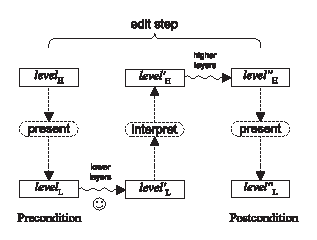
\epsfig{file=pics/eps/LayerSingle.eps, height=1.4in}
\end{center}\caption{Single edit step in a combined layer. (draft)} \label{combinedEdit}
\end{center}
\end{small}
\end{figure}

\note{use of $Present$/$Interpret$ in figure is not entirely correct}
%\begin{figure}
%\xpr{
%level\H 		&   			& level'\H 	&~\rightarrow~& level''\H\\
%~~~\downarrow&   		&~~~\uparrow&			&~~~\downarrow \\
%level\M 		&   			& level'\M 	& 			& level''\M\\
%~~~\downarrow 	&   		&~~~\uparrow&			&~~~\downarrow \\
%level\L 		&~\leadsto~& level'\L 	& 			& level''\L\\
%} \caption{Single edit step in a combined layer. (draft)} \label{combinedEdit}
%\end{figure}

Hence, before the lower level is updated, we have:

\xpr{
\eqcl{\level\L}{LL} = \present\L~\eqcl{\level\M}{LH} ~\land~
\eqcl{\level\M}{HL} = \present\H~\eqcl{\level\H}{HH}\\
\level\L \leadsto \level'\L 
}

After the lower level update, the lower layer computes an intermediate value $\level'\M$, from which the higher layer (which may be a combined layer itself) computes $\level'\H$. At the top, $\level'\H$ is assigned to $\level''\H$, which is subsequently presented onto $level''\M$. Finally, $level''\M$ presented onto $level''\L$. Figure~\ref{combinedEdit} sketches the updates to the various data levels.


\note{add invariant to \law{Doc-Inert} precondition?}
Apart from a few changes to the subscripts, the requirements for $level''\H$ and $level''\L$ are equal to the requirements for the single layer editor in Section~\ref{sect:singleExtra_Editing}. The only difference is that to the precondition of \law{Doc-Inert}, we added the invariant that $\level\L$ is a presentation of $\level\H$, which was not necessary in the previous sections. 

\xprlab{\hoare{\true} {Comp} { \eqcl{\level''\L}{CL} = \present\C~\eqcl{\level''\H}{CH} } }		{Postcondition}
%\xprlab{\hoare{\eqcl{\level\L}{L} = \present\C~\eqcl{\level\H}{H} \land \eqcl{\level'\L}{CL} = %\present\C~\eqcl{\level\H}{CH}} {Comp} { \level\H = \level''\H}}  {Doc-Inert}
\xprlab{ 
\left\{ \begin{array}{l}
 \eqcl{\level\L}{CL} = \present\C~\eqcl{\level\H}{CH} \land\\
 \eqcl{\level'\L}{CL} = \present\C~\eqcl{\level\H}{CH}
\end{array}\right\}
{Comp} \{ \level\H = \level''\H\} }  {Doc-Inert}
\xprlab{\hoare{\eqcl{\level'\L}{CL} = \present\C~\eqcl{h}{CH}} {Comp} { \level'\L = \level''\L}}		{Pres-Inert}
\xprlab{\hoare{\true} {Comp} {\level\H \close \level''\H}}	{Doc-Preserve}
\xprlab{\hoare{\true} {Comp} {\level'\L \close \level''\L}}	{Imprecise}
\note{put supscripts in $Comp$? (eg. $Comp_n$)}

The inductive definition of $Comp$ reads:

\xprlab{
Comp_0 ~~\is~~ 	& \level''\H \gets \level'\H\\
Comp_n ~~\is~~ 	& Up \semi Comp_{n-1} \semi Dwn}{$Comp$-Def}
\xprlab{
Up ~~\is~~		& \level'\M \gets \interpret\L~ \eqcl{\level'\L}{LL}  ~\reuze{LH}~   \level\M}{$Up$-Def}
\xprlab{
Dwn ~~\is~~		& \level''\L \gets \present\L~ \eqcl{\level''\M}{LH}   ~\reuze{LL}~   \level'\L}{$Dwn$-Def}

We prove that $Comp$ meets the requirements.


\head{\law{Postcondition} requirement}

In \fn{wp} notation, the \law{Postcondition} is:

\xprlab{\true ~\imp~ \wp{Comp_n}{\eqcl{\level''\L}{CL} = \present\C~\eqcl{\level''\H}{CH}}} {Postcondition}


\begin{proof} We prove the requirement by induction over the number of layers $n$. 

{\bf Case~} $n=0$

Filling in the base cases for $present\C$, the data levels, and relations $CH$ and $CL$ yields:

\xpr{\true ~\imp~ \wp{Comp}{\eqcl{\level''_0}{=} = \id~\eqcl{\level''_0}{=}}}

which holds because it is equivalent to $\true ~\imp~ \wp{Comp}{\true}$.

{\bf Case~} $n>0$

%\eqcl{l}{CL} = \present\C~\eqcl{h}{CH} & ~\eqv~ & \exists m :~
%			& \eqcl{l}{LL}	& = \present\L~\eqcl{m}{LH}\\
% & &~~\land	& \eqcl{m}{HL}	& = \present\H~\eqcl{h}{HH}
The induction hypothesis is:

\xprlab{\true ~\imp~ \wp{Comp_{n-1}}{ \eqcl{\level''\M}{HL} = \present\H~\eqcl{\level''\H}{HH}}} {I.H.}

In the proof, we need the property that the lower presentation of a valid middle level is in the result of the combined presentation:

\xpr{
\eqcl{m}{HL} = \present\H~\eqcl{h}{HH} ~\imp~ \eqcl{\present~ \eqcl{m}{LH}   ~\reuze{LL}~   l}{CL} = \present\C~\eqcl{h}{CH} \\
}

It has a simple proof:

\begin{Prf}&
	\eqcl{m}{HL} = \present\H~\eqcl{h}{HH} \\
\Eqv{reflexivity of $=$}&
 	\present\L~ \eqcl{m}{LH} = \present\L~\eqcl{m}{LH} \land
 	\eqcl{m}{HL} = \present\H~\eqcl{h}{HH}\\
\Eqv{\law{$\reuz$-Valid}}&
 	\eqcl{\present\L~ \eqcl{m}{LH}   ~\reuze{LL}~   l}{LL} = \present\L~\eqcl{m}{LH} \land
 	\eqcl{m}{HL} = \present\H~\eqcl{h}{HH}\\
\Imp{let $m' = m$}&
 	\exists m' :\eqcl{\present\L~ \eqcl{m}{LH}   ~\reuze{LL}~   l}{LL} = \present\L~\eqcl{m'}{LH} \land
 	\eqcl{m'}{HL} = \present\H~\eqcl{h}{HH}\\
\Eqv{\law{$\present\C$-Def}}&
	\eqcl{\present~ \eqcl{m}{LH}   ~\reuze{LL}~   l}{CL} = \present\C~\eqcl{h}{CH} \\
\end{Prf}


Using this result, we prove \law{Postcondition}.

\begin{Prf}&
	\true\\
\Eqv{\law{\fn{wp}-$\gts$}}&
	\wp{\level'\M \gets \interpret\L~ \eqcl{\level'\L}{LL}  ~\reuze{LH}~   \level\M}{ \true }\\
\Eqv{\law{$Up$-Def}}&
	\wp{Up}{ \true}\\
\Imp{\law{\fn{wp}-Mono} and \law{I.H.}}&
	\wp{Up}{ \wp{ Comp_{n-1}}{  \eqcl{\level''\M}{HL} = \present\H~\eqcl{\level''\H}{HH} }}\\
\Eqv{\law{\fn{wp}-$\smi$}}&
	\wp{Up \semi Comp_{n-1}}{\eqcl{\level''\M}{HL} = \present\H~\eqcl{\level''\H}{HH}} \\
\Imp{\law{\fn{wp}-Mono} and previous result}&
	\wp{Up \semi Comp_{n-1}}{ \eqcl{\present\L~ \eqcl{\level''\M}{LH}   ~\reuze{LL}~   \level'\L}{CL} = \present\C~\eqcl{\level''\H}{CH} }\\
\Eqv{\law{\fn{wp}-$\gts$}}&
	\wp{Up \semi Comp_{n-1}}{ \wp{\level''\L \gets \present\L~ \eqcl{\level''\M}{LH}   ~\reuze{LL}~   \level'\L}{ \eqcl{\level''\L}{CL} = \present\C~\eqcl{\level''\H}{CH} }}\\
\Eqv{\law{$Dwn$-Def}}&
	\wp{Up \semi Comp_{n-1}}{ \wp{Dwn }{ \eqcl{\level''\L}{CL} = \present\C~\eqcl{\level''\H}{CH} }}\\
\Eqv{\law{\fn{wp}-$\smi$}}&
	\wp{Up \semi Comp_{n-1} \semi Dwn}{ \eqcl{\level''\L}{CL} = \present\C~\eqcl{\level''\H}{CH} }\\
\Eqv{\law{$Comp$-Def}}&
	\wp{Comp}{\eqcl{\level''\L}{CL} = \present\C~\eqcl{\level''\H}{CH}}\\
\end{Prf}
\end{proof}






\head{\law{Doc-Inert} requirement}

\xprlab{\eqcl{\level\L}{CL} = \present\C~\eqcl{\level\H}{CH} \land \eqcl{\level'\L}{CL} = \present\C~\eqcl{\level\H}{CH} ~\imp\\ \wp{Comp_n}{\level\H = \level''\H}}{Doc-Inert}

Besides the two conditions specified in Section~\ref{sect:combinedExtra}, we need an additional condition for \law{Doc-Inert} to hold. From \law{InterPresent}, we know that if $\level'\L$ is a presentation of $\level\H$, then $\level\H$ is in the interpretation of $\level'\L$. Thus, there exists a middle level $m$ in the interpretation of $\level'\L$, which has $\level\H$ in its interpretation. However, the mere existence of such a middle level does not guarantee that this is the middle level resulting from $Comp$.

The problem lies in the fact that $level'\M$ is selected by $\reuze{LH}$ from an $LH$ class of elements, instead of an $HL$ class. Thus, reusing extra state from $level\M$ could cause $\level'M$ to end up in an $HL$ class that does not contain $level\M$, which would break \law{Doc-Inert}. We avoid the problem by requiring that the result of $\reuze{LH}$ is in the correct $HL$ class, if possible:

\xprlab{
\eqcl{m'}{HL} = \eqcl{m}{HL} ~\imp~ \eqcl{\eqcl{m'}{LH} \reuze{LH} m}{HL} = \eqcl{m}{HL}}{Orthogonal}

If both $HL$ and $LH$ are described by wildcard types (see Section~\ref{}), \law{Orthogonal} holds.

%
%\xprlab{
%\eqcl{m'}{HL} = \eqcl{m}{HL} ~\imp~ \eqcl{m'}{LH} \reuze{LH} m \in \eqcl{m}{HL}}{Orthogonal}
%
%
%Different notation:
%\xprlab{
%m'~HL~m ~\imp~ \eqcl{m'}{LH} \reuze{LH} m~HL~m}{Orthogonal}



\note{say why it is $HL$ and not $LH$)}
\note{figure out if it is L or CL, etc}

%\xprlab{\hoare{\eqcl{\level'\M}{HL} = \present\H~\eqcl{\level\H}{H}} {Comp_{n-1}} { \level\H = \level''\H}}{I.H.}

\begin{proof}

Th proof is by induction over $n$. 

{\bf Case~} $n=0$

\xpr{\eqcl{\level_0}{=} = \id~\eqcl{\level_0}{=} \land \eqcl{\level'_0}{=} = \id~\eqcl{\level_0}{=} ~\imp~ \wp{Comp_0}{\level_0 = \level''_0}}

%\xpr{\true ~\imp~ \wp{Comp}{\eqcl{\level''_0}{=} = \id~\eqcl{\level''_0}{=}}}

\begin{Prf}&
	\eqcl{\level_0}{=} = \id~\eqcl{\level_0}{=} \land \eqcl{\level'_0}{=} = \id~\eqcl{\level_0}{=}\\
\Eqv{definition of $\id$}&
	\eqcl{\level_0}{=} = \eqcl{\level_0}{=} \land\eqcl{\level'_0}{=} = \eqcl{\level_0}{=}\\
\Imp{reflexivity of $=$ and \law{$\eqhole$-Member}}&
	\level'_0 \in \eqcl{\level_0}{=}\\
\Imp{property of equivalence class and symmetry of $=$}&
	\level_0 = \level'_0\\
\Eqv{\law{\fn{wp}-$\gts$}}&
	\wp{\level''_0 \gets \level'_0}{\level_0 = \level''_0}\\
\Eqv{\law{$Comp$-Def}}&
	\wp{Comp_0}{\level_0 = \level''_0}\\
\end{Prf}


{\bf Case~} $n>0$

For the inductive case, we assume the antecedent of the implication. The first combined $present$ has already been written out according to \law{$\present\C$-Def} and the implicit assumption that the middle level between $level\H$ and $\level\L$ is $level\M$.

\xpr{\eqcl{\level\L}{LL} = \present\L~\eqcl{\level\M}{LH} \land \eqcl{\level\M}{HL} = \present\H~\eqcl{\level\H}{HH} \land\\
 \eqcl{\level'\L}{L} = \present\C~\eqcl{\level\H}{H}}


In the proof, we need the existence of an $m_0$ that is in the interpretation of $\level'\L$ and at the same time in the presentation of $\level\H$:

\begin{Prf}&
	\eqcl{m_0}{LH} = \interpret\L~\eqcl{\level'\L}{LL} \land \eqcl{m_0}{HL} = \present\H~\eqcl{\level\H}{HH}\\
\FFr{let $m_0$ be the $m$ from the quantification}&
	\exists m : \eqcl{m}{LH} = \interpret\L~\eqcl{level'\L}{LL} \land \eqcl{m}{HL} = \present\H~\eqcl{\level\H}{HH}\\
\Eqv{\law{InterPresent}}&
	\exists m : \eqcl{level'\L}{LL} = \present\L~\eqcl{m}{LH} \land \eqcl{m}{HL} = \present\H~\eqcl{\level\H}{HH}\\
\Eqv{\law{$\present\C$-Def}}&
	\eqcl{level'\L}{CL} = \present\C~\eqcl{\level\H}{CH}\\
\Eqv{assumption}&
	\true\\
\end{Prf} \note{how to call the ``let $m_0$ be the $m$ from the quantification'' step? }
          
%\begin{Prf}&
%	\eqcl{m_0}{HL}\\
%\Equ{$\eqcl{m_0}{HL} = \present\H~\eqcl{\level\H}{HH}$}&
%	\present\H~\eqcl{\level\H}{HH}\\
%\Equ{\law{Present}}&
%	\eqcl{\level\M}{HL}\\
%\end{Prf}

Together with $\present\H~\eqcl{\level\H}{HH} = \eqcl{\level\M}{HL}$ from the precondition, $\eqcl{m_0}{HL} = \present\H~\eqcl{\level\H}{HH}$ implies that $m_0$ and $\level\M$ are in the same $HL$ class: $\eqcl{m_0}{HL}=\eqcl{\level\M}{HL}$. This result is needed in order to apply \law{Orthogonal}.

% can be put in linear wp proof
%\begin{Prf}&
%	\eqcl{\interpret~ \eqcl{\level'\L}{LL}  ~\reuze{LH}~   \level\M}{HL}\\
%\Equ{$\eqcl{m_0}{LH} = \interpret\L~\eqcl{\level'\L}{LL}$}&
%	\eqcl{\eqcl{m_0}{LH}   ~\reuze{LH}~   \level\M}{HL}\\
%\Equ{\law{Orthogonal} (different notation) + $\eqcl{m_0}{HL}=\eqcl{\level\M}{HL}$}&
%	\eqcl{m_0}{HL}\\
%\Equ{\law{$\eqcl{m_0}{HL} = \present\H~\eqcl{\level\H}{HH}$}}&
%	\present\H~\eqcl{\level\H}{HH}\\
%\end{Prf}

For the inductive step, we have the following induction hypothesis:

\xprlab{\eqcl{\level\M}{HL} = \present\H~\eqcl{\level\H}{H} \land \eqcl{\level'\M}{HL} = \present\H~\eqcl{\level\H}{H} ~\imp~ \wp{Comp_{n-1}}{\level\H = \level''\H}}{I.H.}

Note that the first part of the conjunction in the antecedent is already satisfied due to the assumption above.

\begin{Prf}&
	\present\H~\eqcl{\level\H}{HH} = \present\H~\eqcl{\level\H}{HH}\\
\Eqv{\law{$\eqcl{m_0}{HL} = \present\H~\eqcl{\level\H}{HH}$}}&
	\eqcl{m_0}{HL} = \present\H~\eqcl{\level\H}{HH}\\
\Eqv{\law{Orthogonal} and $\eqcl{m_0}{HL}=\eqcl{\level\M}{HL}$}&
	\eqcl{\eqcl{m_0}{LH}   ~\reuze{LH}~   \level\M}{HL} = \present\H~\eqcl{\level\H}{HH}\\
\Eqv{$\eqcl{m_0}{LH} = \interpret\L~\eqcl{\level'\L}{LL}$}&
	\eqcl{\interpret~ \eqcl{\level'\L}{LL}  ~\reuze{LH}~   \level\M}{HL} = \present\H~\eqcl{\level\H}{HH}\\
%\end{Prf}
%
%
%\begin{Prf}&
%	\eqcl{\interpret~ \eqcl{\level'\L}{LL}  ~\reuze{LH}~   \level\M}{HL} =  \present\H~\eqcl{\level\H}{HH}\\
\Eqv{\law{\fn{wp}-$\gts$}}&
	\wp{\level'\M \gets \interpret\L~ \eqcl{\level'\L}{LL}  ~\reuze{LH}~   \level\M}{ \eqcl{\level'\M}{HL} = \present\H~\eqcl{\level\H}{HH} }\\
\Eqv{\law{$Up$-Def}}&
	\wp{Up}{ \eqcl{\level'\M}{HL} = \present\H~\eqcl{\level\H}{H}}\\
\Imp{\law{\fn{wp}-Mono}, \law{I.H.}, and $\eqcl{\level\M}{HL} = \present\H~\eqcl{\level\H}{H}$}&
	\wp{Up}{ \wp{ Comp_{n-1}}{ \level\H = \level''\H }}\\
\Eqv{\law{\fn{wp}-$\smi$}}&
	\wp{Up \semi Comp_{n-1}}{ \level\H = \level''\H }\\
\Eqv{\law{\fn{wp}-$\gts$}}&
	\wp{Up \semi Comp_{n-1}}{ \wp{\level''\L \gets \present\L~ \eqcl{\level''\M}{LH}   ~\reuze{LL}~   \level'\L}{ \level\H = \level''\H }}\\
\Eqv{\law{$Dwn$-Def}}&
	\wp{Up \semi Comp_{n-1}}{ \wp{Dwn }{ \level\H = \level''\H }}\\
\Eqv{\law{\fn{wp}-$\smi$}}&
	\wp{Up \semi Comp_{n-1} \semi Dwn}{ \level\H = \level''\H }\\
\Eqv{\law{$Comp$-Def}}&
	\wp{Comp}{\level\H = \level''\H}\\
\end{Prf}
\end{proof}






\head{\law{Pres-Inert} requirement}

\xprlab{\eqcl{\level'\L}{CL} = \present\C~\eqcl{h}{CH} ~\imp~ \wp{Comp_n} { \level'\L = \level''\L}}		{Pres-Inert}

The two conditions from Section~\ref{sect:combinedExtra} are strong enough to guarantee \law{Pres-Inert}. However, the proof of this is very tedious, partly because of the reference to $present\H$ and $interpret\H$ in \law{Sane}. Therefore, we introduce a stronger condition \law{Absorption}, which allows for a simpler proof of \law{Pres-Inert}, and which can be proven to imply the other two conditions, as well as \law{Orthogonal}.

%\xprlab{
%\forall m : \eqcl{m}{LH} \subset \eqcl{m}{HL}}{Absorption}

\xprlab{
\eqcl{m}{LH} = \eqcl{m'}{LH} ~\imp~ \eqcl{m}{HL} = \eqcl{m'}{HL}}{Absorption}

Absorption holds when each $HL$ equivalence class is a union of $LH$ classes. Hence, variations in the $LH$ extra state can never cause a change of the $HL$ equivalence class (and hence never influence the document). 

For wildcard types, \law{Absorption} holds when for each $*$ in the type definition of the $LH$ type the corresponding child in the $HL$ type is also a $*$, or the corresponding type of one of its ancestors is a $*$.  For example, $(Int,(Int,*))$ is absorbed by $(Int,(*,*))$, but also by $(Int,*)$.


\begin{proof}

In the inductive step of the proof, we need the fact that the lower level is not affected by the computations of the higher layer. Therefore, we strengthen the pre- and postcondition of \law{Pres-Inert}: \note{more on this?}

\xpr{ \eqcl{\level'\L}{CL} = \present\C~\eqcl{h}{CH}  \land \level_{n+1} = x ~\imp\\ \wp{Comp_n}{\level'\L = \level''\L  \land \level_{n+1} = x}}

%Here we need:
%
%which implies
%
%\begin{Prf}&
%	\eqcl{\level'\L}{CL} = \present\C~\eqcl{h}{CH}\\
%\Imp{magic}&
%	\eqcl{\level'\L}{CL} = \present\C~\eqcl{h}{CH} \land \level_{n+1} = x\\
%\Imp{assumption}&
%	\wp{Comp_n}{\level'\L = \level''\L  \land \level_{n+1} = x}\\
%\Imp{\law{\fn{wp}-Mono} and $X \land Y ~\imp~ X$}&
%	\wp{Comp_n}{\level'\L = \level''\L}\\
%\end{Prf}


{\bf Case~} $n=0$

\xpr{\eqcl{\level'_0}{H} = \present~\eqcl{h}{H} \land \level_{1} = x ~\imp~\wp {Comp_0} { \level'_0 = \level''_0 \land \level_{n+1} = x}}

evident from def of $Comp_0$:

\xpr{\hoare{\eqcl{\level'_0}{H} = \present~\eqcl{h}{H}} {\level''_0 \gets \level'_0} { \level'_0 = \level''_0}}

%\xpr{\hoare{\eqcl{\level'\L}{L} = \present~\eqcl{h}{H}} {Comp_n} { \level'\L = \level''\L}}


%\xpr{ \eqcl{\level'_0}{H} = \present_0~\eqcl{h}{H} ~\imp~ \wp{Comp_0}{\level'_0 = \level''_0}} 
%
%\begin{Prf}
%\Eqv{\law{\fn{wp}-$\gts$}}&
%	\wp{\level''\H \gets \interpret~\level'\L}{ \wp{ \level''\L \gets \present~\level''\H}{\level\H = \level''\H}} \\
%\Eqv{\law{\fn{wp}-$\smi$}}&
%	\wp{\level''_0 \gets \level'_0}{\level_0 = \level''\H} \\
%\Eqv{\law{$Comp$-Def}}&
%	\wp{Comp_0}{\level'_0 = \level''_0}\\
%\end{Prf}

{\bf Case~} $n>0$

First we prove the first part of postcondition conjunct:

\xpr{ \eqcl{\level'\L}{CL} = \present\C~\eqcl{h}{CH} \land \level_{n+1} = x  ~\imp~ \wp{Comp_n}{\level'\L = \level''\L}}

We only need to assume half of the antecedent:
 $\eqcl{\level'\L}{CL} = \present\C~\eqcl{h}{CH}$.


%result of $Up$ and $m_0$ are in same LH class.
%
%does not seem to work:
%\begin{Prf}&
%	(\interpret\L~ \eqcl{\level'\L}{LL})  \reuze{LH}   \level\M  \\
%\Eqv{$\eqcl{m_0}{LH} = \interpret\L~\eqcl{level'\L}{LL}$}&
%	\eqcl{m_0}{LH}  \reuze{LH}   \level\M  \\
%\Imp{\law{$\reuz$-Valid}}&
%	\eqcl{m_0}{LH}\\
%\Imp{\law{Absorption}}&
%	\level'\M \in \eqcl{m_0}{HL}\\
%\Imp{\law{$\eqhole$-Member}}&
%	\eqcl{\level'\M}{HL} = \eqcl{m_0}{HL}\\
%\end{Prf}
%\note{rewrite valid? or just mention that it can be rewritten (as = on eq. classes)}
%\xpr{
%\eqcl{\interpret~ \eqcl{\level'\L}{L}  ~\reuze{H}~  \level\M}{HL} = \present\H~\eqcl{h}{HH} \\
%}


From the assumption, we know there exist an $m_0$ that is in the presentation of $h$, and that has $\level'\L$ in its presentation:

\begin{Prf}&
	\eqcl{level'\L}{LL} = \present\L~\eqcl{m_0}{LH} \land \eqcl{m_0}{HL} = \present\H~\eqcl{h}{HH}\\
\Eqv{let $m_0$ be the $m$ from the quantification}&
	\exists m : \eqcl{level'\L}{LL} = \present\L~\eqcl{m}{LH} \land \eqcl{m}{HL} = \present\H~\eqcl{h}{HH}\\
\Eqv{\law{$\present\C$-Def}}&
	\eqcl{level'\L}{CL} = \present\C~\eqcl{h}{CH}\\
\Eqv{assumption}&
	\true\\
\end{Prf}

Furthermore, by the first part of this conjunct and \law{InterPresent} on the lower layer, we also have $\eqcl{m_0}{LH} = \interpret\L~\eqcl{level'\L}{LL}$
%$\eqcl{m_0}{HL} = \present\H~\eqcl{h}{HH}$


%Define an $m'$ to be $(\interpret\L~ \eqcl{\level'\L}{LL})  \reuze{LH}   \level\M$
%\begin{Prf}&
%	\true\\
%\Eqv{ bla }&
%	m' = (\interpret\L~ \eqcl{\level'\L}{LL})  \reuze{LH}   \level\M  \\
%\Imp{$\eqcl{m_0}{LH} = \interpret\L~\eqcl{level'\L}{LL}$}&
%	m' = \eqcl{m_0}{LH}  \reuze{LH}   \level\M  \\
%\Imp{\law{$\reuz$-Valid}}&
%	m' \in \eqcl{m_0}{LH}\\
%\Imp{\law{Absorption}}&
%	m' \in \eqcl{m_0}{HL}\\
%\Imp{\law{$\eqhole$-Member}}&
%	\eqcl{m'}{HL} = \eqcl{m_0}{HL}\\
%\Eqv{\law{$\eqhole$-Member}}&
%	\eqcl{(\interpret\L~ \eqcl{\level'\L}{LL})  \reuze{LH}   \level\M}{HL} = \eqcl{m_0}{HL}\\
%\end{Prf}

%or alternatively: using rewritten \law{Absorption}
%\eqcl{m}{LH} = \eqcl{m'}{LH} ~\imp~ \eqcl{m}{HL} = \eqcl{m'}{HL}}{Absorption}
We need two intermediate results for the inductive step of the proof. The first one is:

\begin{Prf}&
	\eqcl{\interpret~ \eqcl{\level'\L}{L}  ~\reuze{LH}~  \level\M}{HL} = \present\H~\eqcl{h}{HH} \\
\Equ{$\eqcl{m_0}{HL} = \present\H~\eqcl{h}{HH}$}&
	\eqcl{\interpret\L~ \eqcl{\level'\L}{LL}  \reuze{LH}   \level\M}{HL} = \eqcl{m_0}{HL}\\
\Ffr{\law{Absorption}}&
	\eqcl{\interpret\L~ \eqcl{\level'\L}{LL}  \reuze{LH}   \level\M}{LH} = \eqcl{m_0}{LH}\\
\Eqv{$\eqcl{m_0}{LH} = \interpret\L~\eqcl{level'\L}{LL}$}&
	\eqcl{\eqcl{m_0}{LH}  \reuze{LH}   \level\M}{LH} = \eqcl{m_0}{LH}\\
\Eqv{\law{$\reuz$-Valid}}&
	\eqcl{m_0}{LH} = \eqcl{m_0}{LH}\\
\Eqv{reflexivity of $=$}&
	\true\\
\end{Prf}

A corollary from this proof is that $\eqcl{\interpret\L~ \eqcl{\level'\L}{LL}  \reuze{LH}   \level\M}{LH} = \eqcl{m_0}{LH}$, which is used in the proof of the second intermediate result:
% this used to be a separate proof
%For the first equality in conjunct:
%\xpr{
%\eqcl{\interpret~ \eqcl{\level'\L}{L}  ~\reuze{LH}~  \level\M}{HL} = \present\H~\eqcl{h}{HH} \\
%}
%
%\begin{Prf}&
%	\eqcl{(\interpret\L~ \eqcl{\level'\L}{LL})  \reuze{LH}   \level\M}{HL}\\
%\Equ{previous result}&
%	\eqcl{m_0}{HL}\\
%\Equ{$\eqcl{m_0}{HL} = \present\H~\eqcl{h}{HH}$}&
%	\present\H~\eqcl{h}{HH}\\
%\end{Prf}


\xpr{
\level'\L = \present~ \eqcl{\interpret~ \eqcl{\level'\L}{LH}  ~\reuze{LH}~  \level\M}{LH}   ~\reuze{LL}~   \level'\L\\
}

\begin{Prf}&
	\level'\L\\
\Equ{\law{$\reuz$-Idem} and $\eqcl{level'\L}{LL} = \eqcl{level'\L}{LL}$}&
	\eqcl{level'\L}{LL}  \reuze{LL}  \level'\L\\
\Equ{$\eqcl{level'\L}{LL} = \present\L~\eqcl{m_0}{LH}$}&
	\present\L~ \eqcl{m_0}{LH}  \reuze{LL}  \level'\L\\
\Equ{corollary: $\eqcl{\interpret~ \eqcl{\level'\L}{L}  ~\reuze{H}~  \level\M}{LH} = \eqcl{m_0}{LH}$}&
	\present\L~ \eqcl{\interpret~ \eqcl{\level'\L}{L}  ~\reuze{LH}~  \level\M}{LH}  \reuze{LL}  \level'\L\\
\end{Prf}

Now we can prove the inductive step with induction hypothesis:

\xprlab{\eqcl{\level'\M}{HL} = \present\H~\eqcl{h}{HH} ~\imp~ \wp{Comp_{n-1}}{\level'\M = \level''\M}}{I.H.}

%\xpr{
%	\begin{array}[b]{@{}l@{}l@{}l}
%	 \eqcl{\interpret\L~ \eqcl{\level'\L}{L}  ~\reuze{H}~  \level\M}{HL} = \present\H~\eqcl{h}{HH} \land\\
%	 \level'\L = \present\L~ \eqcl{\interpret\L~ \eqcl{\level'\L}{L}  ~\reuze{H}~  \level\M}{LH}   ~\reuze{L}~   \level'\L\\
%	\end{array}\\
%	 }

The proof starts with the conjunction of the two intermediate results that we just proved.

\begin{Prf}
  &	\eqcl{\interpret\L~ \eqcl{\level'\L}{LL}  ~\reuze{LH}~  \level\M}{HL} = \present\H~\eqcl{h}{HH} ~~\land\\
  &	\level'\L = \present\L~ \eqcl{\interpret\L~ \eqcl{\level'\L}{LL}  ~\reuze{LH}~  \level\M}{LH}   ~\reuze{LL}~   \level'\L\\
\Eqv{\law{\fn{wp}-$\gts$}}&
	\fn{wp}( \level'\M \gets \interpret\L~ \eqcl{\level'\L}{LL}  ~\reuze{LH}~  \level\M,\\
 & \hspace{0.7cm} \eqcl{\level'\M}{HL} = \present\H~\eqcl{h}{HH} \land \level'\L = \present\L~ \eqcl{\level'\M}{LH}   ~\reuze{LL}~   \level'\L ) \\
\Eqv{\law{$Up$-Def}}&
	\wp{Up}{ \eqcl{\level'\M}{HL} = \present\H~\eqcl{h}{HH}  ~~\land \level'\L = \present\L~ \eqcl{\level'\M}{LH}   ~\reuze{LL}~   \level'\L}\\
\Imp{\law{\fn{wp}-Mono} and \law{I.H.}}&
	\wp{Up}{ \wp{ Comp_{n-1}}{ \level'\M = \level''\M ~~\land \level'\L = \present\L~ \eqcl{\level'\M}{LH}   ~\reuze{LL}~   \level'\L}}\\
\Eqv{\law{\fn{wp}-$\smi$}}&
	\wp{Up \semi Comp_{n-1}}{  \level'\M = \level''\M ~~\land \level'\L = \present\L~ \eqcl{\level'\M}{LH}   ~\reuze{LL}~   \level'\L}\\
\Imp{\law{\fn{wp}-Mono} and $x = x' \land P (x) ~~\imp~~ P (x')$}&
	\wp{Up \semi Comp_{n-1}}{ \level'\L = \present\L~ \eqcl{\level''\M}{LH}   ~\reuze{LL}~   \level'\L}\\
\Eqv{\law{\fn{wp}-$\gts$}}&
	\wp{Up \semi Comp_{n-1}}{ \wp{\level''\L \gets \present\L~ \eqcl{\level''\M}{LH}   ~\reuze{LL}~   \level'\L}{ \level'\L = \level''\L }}\\
\Eqv{\law{$Dwn$-Def}}&
	\wp{Up \semi Comp_{n-1}}{ \wp{Dwn }{ \level'\L = \level''\L }}\\
\Eqv{\law{\fn{wp}-$\smi$}}&
	\wp{Up \semi Comp_{n-1} \semi Dwn}{ \level'\L = \level''\L }\\
\Eqv{\law{$Comp$-Def}}&
	\wp{Comp}{\level'\L = \level''\L}\\
\end{Prf}

This completes proof of:

\xpr{ \eqcl{\level'\L}{CL} = \present\C~\eqcl{h}{CH} \land \level_{n+1} = x  ~\imp~ \wp{Comp_n}{\level'\L = \level''\L}}

Because $Comp_n$ only does assignments on levels $0 \dots n$, we also have:

\xpr{ \eqcl{\level'\L}{CL} = \present\C~\eqcl{h}{CH} \land \level_{n+1} = x ~\imp~ \wp{Comp_n}{\level_{n+1} = x}}

Hence, by \law{\fn{wp}-And}, we can conclude: 

\xpr{ \eqcl{\level'\L}{CL} = \present\C~\eqcl{h}{CH}  \land \level_{n+1} = x ~\imp~ \wp{Comp_n}{\level'\L = \level''\L  \land \level_{n+1} = x}}

\end{proof}



%Story on compatibility here? Or in conclusions?
%
%Explanation compatible. Even if h exists, moving in lower med eq. class could lead to levelH not in [h] (probably must be an %imprecise edit). This would cause $l$ update. 
%
%In order to prevent, for all variation we require validity (and hence by pres-inert stay in correct class), or if invalid, at least stay %in same class.
%
%
%Compatibility (obsolete):

%% old version:
%%\xprlab{
%%\forall m_0 : & (\exists m \in \eqcl{m_0}{LH} : \exists h: m~Present~h) \imp\\
%%                   & \begin{array}[b]{@{}l@{}l@{}l}
%%                      \forall m' \in \eqcl{m_0}{LH} :~&  (\exists h_0 : \eqcl{m'}{HL} = pres \eqcl{h_0}{HH})~\lor\\
%%                    							& (\present\H \oo \interpret\H) \eqcl{m'}{HL} \subset 			\end{array}
%%\eqcl{m_0}{LH}}{Compatible}
%%
%%or if we define: $\valid~l \eqv \exists h : \eqcl{l}{L} \present \eqcl{h}{H}$ (note that this is on {\em a} layer, not on higher %%or lower)
%%
%%\xprlab{
%%\forall m_0 : & (\exists m \in \eqcl{m_0}{LH} : \valid~m) \imp\\
%%                   & \begin{array}[b]{@{}l@{}l@{}l}
%%                       \forall m' \in \eqcl{m_0}{LH} : ~ & \valid~m'~\lor\\
%%									&(\present\H \oo \interpret\H) \eqcl{m'}{HL} \subset \eqcl{m_0}{LH}
%%			\end{array}
%%}{Compatible}
%%
%%Lambert:
%%\xprlab{
%%\forall m_0 : \forall m,m' : \valid~m \land \lnot \valid~m' ~~\imp \dots \subset \dots
%%}

%\xprlab{
%\forall m_0 : & (\exists m \in \eqcl{m_0}{LH} : \valid~m) \imp\\
%                   & \begin{array}[b]{@{}l@{}l@{}l}
%                       & \valid~m_0~\lor\\
%			&(\present\H \oo \interpret\H) \eqcl{m_0}{HL} \subset \eqcl{m_0}{LH}
%			\end{array}
%}{Compatible}
%
%



\head{\law{Imprecise} and preservation of extra state requirement}

\toHere

\bl
\o Is this the case when m'' is close to m and l'' is close to l, for the individual layers? Or is there an m'' that is not closest to m, but for which pres m is closest to l?
\o do es reqs also say something about middle es?
\el



\subsection{Conclusions}


Absorption means that all higher es of lower layer gets absorbed by layer above. So only the highest layer can have doc extra state. This seems to strict.

Problem: in one eq. class, can there be several situations? eg (*,*) \dbarr (), one absorbed, the other always valid (or other condition)

Conditions on composing layers:

***

\xprlab{
\eqcl{m'}{HL} = \eqcl{m}{HL} ~\imp~ \eqcl{\eqcl{m'}{LH} \reuze{LH} m}{HL} = \eqcl{m}{HL}}{Orthogonal}


Or: 

\xprlab{
\eqcl{m}{LH} = \eqcl{m'}{LH} ~\imp~ \eqcl{m}{HL} = \eqcl{m'}{HL}}{Absorption}

But this one is very strong. We would like to find a less strict condition.

Maybe different approach for handling imprecise edit will help.

\bl
\o In Proxima, only pres ES in lower layer and interpretation extra state in top.
\o Putting doc extra state only in upper layer seems to prevent most problems.
\el



\fromHere
%																
%																
%																
\section{Duplicate presentations} \label{sect:duplicates}
\note{call them dependent values rather than duplicates?}
% Introduction
The specification developed in the previous sections is suitable for describing a large class of editors, but still lacks support for presentations that duplicate information. A simple example of a duplicate presentation is the function $\present~x = (x, x)$. An intuitive way to handle edit operations on duplicates is to let the edited duplicate determine the document update. However, this behavior cannot be expressed by the specifications in the previous sections, since the specification does not take into account the original $level\L$.

Duplicates become especially problematic in the combination with extra state and multiple layers. In fact, the pathological cases that give rise to the extra conditions in Section~\ref{sect:combinedExtraCompose} all contain some form of duplication.  \note{add refs on duplicates from DB and inversion papers}

In this section, we discuss how the specification can be adapted to support the handling of duplicate presentations. Although we have established a tentative specification of when exactly a presentation contains duplicates, it is still requires much improvement. Therefore, the remainder of this section is of an informal nature.
\note{spec is hard without making additional assumptions on the pres. formalism}
% close on document gets into trouble with pres-inert

\subsection{Dealing with duplicates}


% what are duplicates
Besides the obvious $\present~x = (x, x)$, we also speak of duplication when a presentation contains a value together with a value that is derived from it (eg. $\present~x = (x, -x)$). This holds even if computation for the derived value does not have an inverse, as in $\present~x = (x, x~\fn{mod}~256)$.  A related example $\present~x = (x~\fn{div}~256, x~\fn{mod}~256)$ shows the subtlety of duplication, since in this case there is no duplication of information. 

Besides depending on a single document value, a duplicate may also depend on several values. Hence, an average value of a list of integers can be regarded as a duplication of the values in the list.\note{term duplicates seems a bit odd here} Other examples of duplication are derived type signatures for functions, or even the color of a keyword in a syntax-coloring editor.

% another one: $1 \to "one"$ can be seen as three partial duplicates. 
% what's this note? parsing with correction. ??? 


% simple solution
The easiest way to deal with duplicate information is to simply ignore one of the duplicates on interpretation and thereby rendering the ignored duplicate non-editable. This is in fact the only way that is allowed by the specification of the previous sections. For $\present~x = (x,x)$, this leaves a choice of interpret functions: with $\interpret~(x,y) = x$, only the left value is editable, and with $\interpret~(x,y) = y$ only the right value.

In some cases non-editable duplicates are perfectly acceptable. In case of the list of integers with its average, few people will expect to be able to edit the average value. And perhaps even fewer people will expect to be able to edit colors in a syntax-coloring editor and thereby modify the edited program source. However, in some cases we do want to be able to edit duplicate values.

\subsection{Adapting the \law{Imprecise} requirement}
% This is not consistent with ``close to'' on presentation.  
% If $(1,1) \leadsto (1,8)$ then $(8,8)$ is probably closer as far as the user is concerned.
Instead of ignoring one of the duplicates, a more user-friendly approach is to use the value of the changed duplicate to determine the document update. This is in line with the requirement that if an update is imprecise, the editor will perform the operation that the user intended. 

\note{not entirely true if we block out duplicates}
Edit operations on duplicates most probably result in an invalid presentation, unless a user has managed to consistently edit all appearences of the duplicate. Hence, the result of an edit operation on a duplicate value is mainly specified by the \law{Imprecise} requirement: 

%The problem with duplicates is that information from the document is present several times in the presentation.
%We tackle the problem by taking the 

\xprlab{\hoare{\true} {Comp} {\level'\L \close \level''\L}}	{Imprecise}

However, in its current form, \law{Imprecise} cannot specify the desired behavior, since it relates $\level''\L$ to $\level'\L$ without taking $\level\L$ into account. An example shows the problem that can occur.

Consider an editor with $\present~x = (x,x)$. Because the edit operation $(0,0) \leadsto (1,0)$, should result in the presentation $(1,1)$, we must have $(1,0) \close (1,1)$. On the other hand the desired result of $(1,1) \leadsto (1,0)$ should be $(0,0)$, implying $(1,0) \close (0,0)$. Because it does not refer to $\level\L$, \law{Imprecise} cannot specify the desired behavior.

%Hence, the value of $\interpret (1,0)$ depends not only on $\level'\L$, but also on the $level\L$.

A second example shows more precisely what the problem is. Consider the function 
$\present~x = (x,x,x)$. If a user edits the first element of the presentation
($(0,0,0) \leadsto (1,0,0)$) the intuitive result would be to change the document to $1$. However, since $(1,0,0)$ is arguably closer to $(0,0,0)$ than $(1,1,1)$, $level''\H$ is specified to be $0$ instead of $1$. Therefore, an editor conforming to the specification does not allow any editing in the presentation, unless two or more values are edited simultaneously and consistently. 


% just looking at change is not really enough. 
The problem with the \law{Imprecise} requirement is that the duplicates of the edited part of the presentation influence the final result of the edit operation. We tackle the problem by introducing an operator to ignore these duplicates:

\xpr{
\Delta \tp  T \to T \to T\st\\
}

The result of $x~\Delta~x'$ is a value that is structurally the same as $x'$, but in which the duplicates of the parts that are different from $x$ have been replaced wildcards ($*$). Thus, for a presentation without duplicates, we have $x \Delta x' = x'$. 
If two duplicates are updated simultaneously, the result of $\Delta$ is not defined.

Similar to Section~\ref{sect:wildcardEq}, a wildcard stands for any value, and therefore can be ignored when testing for equality, or evaluating closeness. Hence, $(1,*,*)$ is maximally close to $(1,1,1)$, but also to $(1,3,5)$, for example.

We give two examples to illustrate the behavior of $\Delta$. Let $\present~(x,y) = (x,x,y)$, then 
$(1,1,5)~\Delta~(1,2,5) = (*,2,5)$ and $(3,1,5)~\Delta~(1,2,5) = (3,*,5)$, but $(1,1,5)~\Delta~(1,1,4) = (1,1,4)$. Another example is $\present~(x,y) = (x,y,x+y)$, with $(1,2,3)~\Delta~(10,2,3) = (10,2,*)$ and 
$(1,2,3)~\Delta~(1,2,13) = (1*,*,12)$. 


Unfortunately, it is difficult to give a formal specification of $\Delta$, as we have not established a formal description of dependencies between values yet. Furthermore, when a value influences the structure of presentation, rather than a specific value in the structure, this cannot be modeled with wildcards. For these reasons, we keep the description of $\Delta$ informal, and leave the behavior of the editor unspecified in conflict situations.


\note{say a bit more about structural diffs?}


%Can we give a definition? Nope
%
%\xpr{
%\Delta \tp  T \to T \to T\st\\
%C~x\st_0 \dots x\st_n =\st C~y_0 \dots y_n ~=~ x\st_0 = y_0 \land \dots \land x\st_n  = y_n\\
%C~x\st_0 \dots x\st_n =\st C'~y_0 \dots y_m ~=~ \false\\
%}
%what about constructors? what about Bin 1 2 $\leadsto$ Bin 0 (Bin 1 2)  Bin 0 * ?
%Lists? same story with subobj. identities?

%
%\xpr{
%=\st ::  T\st \to T \to T\\
%* =\st  y ~=~ \true\\
%C~x\st_0 \dots x\st_n =\st C~y_0 \dots y_n ~=~ x\st_0 =\st y_0 \land \dots \land x\st_n =\st y_n\\
%C~x\st_0 \dots x\st_n =\st C'~y_0 \dots y_m ~=~ \false\\
%}{$\st$-Def}
%
%don't use = core, because we have no data def. Closeness between a wildcard value and an ordinary value is similar. 
%
%``close to'' on $T\st$ and $T$ is similar to $=\st$. everything is close to a $*$.

Using $\Delta$, we define an \law{Imprecise} requirement that does not require closeness on duplicates of the edited part of the presentation:

\xprlab{\hoare{\true} {Comp} {\level\L ~\Delta~\level'\L \close \level''\L}}	{Imprecise}

However, this is requirement alone is not sufficient. Recall that the old \law{Imprecise} also served to preserve the presentation extra state. Because duplicates are ignored by the new \law{Imprecise}, it says nothing about their extra state. Therefore, we need to add a weaker requirement for preserving extra state of the duplicates. The new requirement corresponds to the old \law{Imprecise} requirement:

\xprlab{\hoare{\true} {Comp} {\level'\L \close \level''\L}}	{Pres-Preserve}

With the new requirements, the two examples do not cause any problems anymore. For the $present~x = (x,x)$ example, after $(0,0) \leadsto (1,0)$ the requirement states $(1,*) \close level''\L$, with $(1,1)$ as a solution, whereas for $(1,1)\leadsto (1,0)$ it states $(*,0)$, with $(0,0)$, as a solution. For the triple presentation, the requirement after updating the first element states $(1,*,*) \close level''\L$, which has $(1,1,1)$ as a solution. \note{mention here already that these examples no longer fall under \law{imprecise} when \law{Pres-Inert} is updated? }

\subsection{Adapting the \law{Pres-Inert} requirement}

Besides the \law{Imprecise} requirement, also the \law{Pres-Inert} requirement needs to be adapted to support duplicates. An example shows the problem that can occur with the old \law{Pres-Inert} requirement.

Consider an editor for a very simple functional language. The document type is a list of declarations, which is presented as a list of strings together with a message about type correctness. Furthermore, the body of a function may be hidden (see Section~\ref{sect:sourceeditor}), in which case it is represented by the string \verb|"..."|. 

A type correct document $[f = a+2, a = 1]$, can be presented while hiding the body of $f$, yielding: \verb|"f = ...; a = 1;    ok"|. In the presentation, the string \verb|ok| signals that the program is type correct. 

If a user performs the update $a = 1 \leadsto a = True$, the most logical result would be an updated document 
$[f = a+2, a = True]$, with a presentation that shows the type error: \verb|"f = ...; a = True;    error"|. Of course, in a real-world editor we would like to have a somewhat more informative error message, but this basic message is sufficient for our example.

The problem that occurs is that because $level'\L$ (\verb|"f = ...; a = True;    ok"|) is a valid presentation (consider for example the document  $[f = 2, a = True]$), \law{Pres-Inert} states that $level'\L = level''\L$. This would entail a document update to 
$[f = 2, a = True]$ or something similar, which is clearly not the desired behavior.

%\bl
%\o Pres-Inert suggests to update the hidden parts of the document!
%\el

%
%a = 1; f = a + 2;                                    a = True; f = a + 2              or   a = True; f = undefined
%
%a = 1; f = ...            a = True; f = ...     a = True; f = ... [type err]          a = True; f = ...
%                                *    True   *  

To prevent \law{Pres-Inert} from suggesting updates on hidden parts of the document, we adapt the requirement in a similar way as \law{Imprecise}; both the pre- and the postcondition are changed to ignore duplicates of the updated parts of the lower level:

%\note{Alternatively, could we make \law{Pres-Inert} weaker than \law{Doc-Preserve}?}
% no, pres inert usually conflicts with doc-preserve, making it weaker would disable it.

\xprlab{\hoare{\eqcl{\level\L ~\Delta~\level'\L}{L} =\st \present~\eqcl{h}{H}} {Comp} { \level\L ~\Delta~\level'\L =\st \level''\L}}		{Pres-Inert}

The precondition needs to be weakened because otherwise the presence of duplicates in the presentation may disable the requirement. The postcondition, on the other hand, is weakened because we only require the updated parts to stay the same. Duplicates of the updated part, such as the type error in the example above, may change.

\note{say something about delta in precondition, plus the fact that it is on equivalence class.}

Now that we have updated \law{Pres-Inert}, the two examples from the previous section ($\present x = (x,x)$ and 
$\present~x =(x,x,x)$) no longer fall under the \law{Imprecise} requirement. 


\subsection{The remaining requirements}

The other requirements (\law{Postcondition}, \law{Doc-Inert}, and \law{Doc-Preserve}) do not need to be updated . The postcondition should still hold between the entire higher and lower level, and \law{Doc-Preserve} only refers to higher level values and therefore is not affected by duplicates in the presentation.

The precondition of \law{Doc-Inert} could be changed in a similar way as the precondition of \law{Pres-Inert}, but this is not necessary. Because the precondition ensures that the unchanged parts of the presentation are valid with respect to $\level\H$, only the changed parts may break the precondition. Hence it makes no difference to also include the unchanged parts in the precondition, as the changed parts determine whether it holds or not.

\subsection{Conclusions}

Summarizing, we have the following set of requirements:

\xprlab{\hoare{\true} {Comp} { \eqcl{\level''\L}{L} = \present~\eqcl{\level''\H}{H} } }		{Postcondition}
\xprlab{\hoare{\eqcl{\level'\L}{L} = \present~\eqcl{\level\H}{H}} {Comp} { \level\H = \level''\H}}  {Doc-Inert}
\xprlab{\hoare{\eqcl{\level\L ~\Delta~\level'\L}{L} =\st \present~\eqcl{h}{H}} {Comp} { \level\L ~\Delta~\level'\L = \level''\L}}		{Pres-Inert}
\xprlab{\hoare{\true} {Comp} {\level\L ~\Delta~\level'\L \close \level''\L}}	{Imprecise}
\xprlab{\hoare{\true} {Comp} {\level'\L \close \level''\L}}	{Pres-Preserve}
\xprlab{\hoare{\true} {Comp} {\level\H \close \level''\H}}	{Doc-Preserve}

If the presentation does not contain duplicates, then the requirements correspond exactly to the requirements of the previous section.


\toHere

\bl
\o Duplicates are tricky
\o Easy to make impossible situations, but not a design requirement to solve these. Simple things should be possible.
\o more research on specifying duplicate values
\o How Proxima duplicates
\el



%%%%%%%%% Choice crap:

%\bl
%\o Choice in $\interpret$ may be due to duplicates or '???'
%\o $type Document = Int$ 
%\o ???: $\present x = 2x$ also with several interprets: $\interpret 1 = 0 or 1$ 
%\o Hard to distinguish between the two.
%\o A difference seems to be that using stars on other fields but the edited one, make a non-ambiguous \interpret possible in the %duplication case, but not in the other case. eg. $\interpret (1,*,*) = 1$
%\o Old statement: if there are several choices for \interpret, which all obey \law{InterPresent}, then there are duplicates. This %does not seem to be true. (eg. $\present n = 2n$)
%\el





%																
%																
%																
%\section{Incrementality}
%Informal. Maybe leave this one out


%																
%																
%																
%\section{Loose ends}
%\bl
%\o what about error nodes in document?
%\o what about inserting pres elts that resemble a chapter title? Is this handled well?
%\o difference between {\em presentation extra state} and {\em interpretion extra state}
%\o what if present is not total?
%\el


%																
%																
%																
%\section{document editing}
%
%
%Skipping lower layers
%
%update (pres upd) pres \rarr pres'
%update (doc upd) pres \rarr pres$\times$(doc upd) , which interprets to (update (doc upd) doc)


%																
%																
%																
%\section{layer skipping}
%
%
%Skipping higher layers. Probably won't say much about that here.

\subsection{Related work and conclusions}

\bl
\o Related:
\o all are just simple functions, map, zip, dup, etc. Nothing scaleable yet.
\o Lambert: combinators for specifying maintainers. no expl. model for es \cite{meertens98maintainers}
\o \cite{muhu04inv}
\o Pierce  extra stuff only in one direction. \cite{pierce03lenses}
\el


Do we need additional sections about subjects below?
\bl
\o Document editing
\o Layer skipping
\o incrementality
\el



Always possible to find pathological cases.
We try to define what's a natural editor
%New things may break old. But parts remain valid

Conditions: maybe weaker ones are possible. these are for the most general case.

Future: specification formalism for presentation mappings that guarantees correctness of editors. 
Will need annotations for more complex cases)
% restore old defs from thesis.sty




\pagebreak
\section{Appendix with nasty proofs}



A combined layer defines two relations ($Present\C$ and $Interpret\C $) from four component relations ($Present\H$, $Present\L$, $Interpret\H$, and $Interpret\L$):

\xpr{
Present\C = Present\L \oo Present\H\\
Interpret\C = Interpret\H \oo Interpret\L\\
}

We know that the four component relations are mappings between equivalence classes: 

\xpr{
\present\H   &\tp& \Eqcl{\Level\H}{HH} \rightarrow  \Eqcl{\Level\M}{HL} ~~~\text{and}~~~
\present\L    &\tp& \Eqcl{\Level\M}{LH} \rightarrow  \Eqcl{\Level\L}{LL}\\
\interpret\H   &\tp& \Eqcl{\Level\M}{HL} \rightarrow  \Eqcl{\Level\H}{HH} ~~~\text{and}~~~
\interpret\L   &\tp& \Eqcl{\Level\L}{LL} \rightarrow  \Eqcl{\Level\M}{LH}\\
}

We also wish to regard the combinations as mappings between equivalence classes:

\xpr{
\present\C &\tp& \Eqcl{\Level\H}{CH} \rightarrow  \Eqcl{\Level\L}{CL}~~~\text{and}~~~
\interpret\C &\tp&  \Eqcl{\Level\L}{CL} \rightarrow \Eqcl{\Level\H}{CH}\\
}

However, the counter-example from Section~\ref{sect:combinedExtraCompose} shows this is not necessarily true.

If we want to regard the combination as an equivalence class mapping, we need two things:

Firstly, $Present\C$ must establish an equivalence relation $CH_{\, \mathrm P}$ on $Level\H$ and a relation $CL_{\, \mathrm P}$ on the valid subset of $\Level\L$. Analogously, $Interpret\C$ must establish an equivalence relation $CH_{\, \mathrm I}$ on $Level\H$ and $CL_{\, \mathrm I}$ on $Level\L$ (including the subset that is not valid).

Secondly, the equivalence relations established by $Present\C$ must be equal to the relations established by $Interpret\C$. Hence, we need $CH_{\, \mathrm P} = CH_{\, \mathrm I}$, as well as  $CL_{\, \mathrm P} = CL_{\, \mathrm I}$ for the valid subset of $Level\L$.

Two conditions on the layer components are required for the statements above to hold:

\xprlab{
\forall m, m' : \eqcl{m}{LH} = \eqcl{m'}{LH} \imp & \exists m_1, m'_1 : \eqcl{m_1}{LH} = \eqcl{m'_1}{LH} \\
& \land \eqcl{m_1}{HL} = \present\H (\interpret\H \eqcl{m}{HL})\\
& \land \eqcl{m'_1}{HL} = \present\H (\interpret\H \eqcl{m'}{HL})\\
}{Sane}

and

\xprlab{
\valid~x \land \valid~y \land \eqcl{x}{LH} = \eqcl{y}{LH} \land \eqcl{x}{HL} = \eqcl{x'}{HL} ~\imp\\ 
\exists z : \eqcl{z}{HL} = \eqcl{y}{HL} \land \eqcl{z}{LH} = \eqcl{x'}{LH}
}{Commute}

But because of the complexity of these conditions, we use a stronger condition, that implies \law{Sane} and \law{Commute}:

\xprlab{
\eqcl{m}{LH} = \eqcl{m'}{LH} ~\imp~ \eqcl{m}{HL} = \eqcl{m'}{HL}}{Absorption}

\law{Absorption} also implies \law{Orthogonal}, which is needed in Section~\ref{sect:combinedExtraEditing} for \law{Doc-Inert}.

The next sections contain the proofs of these statements:

\begin{itemize}
\item $Present\C$ and $Interpret\C$ establish equivalence relations. (Section~\ref{eqclassMappings})
\item Relations $Present\C$ of are equal to those of $Interpret\C$. (Section~\ref{presIntrEqual})
\item \law{Absorption} implies  \law{Commute}, \law{Sane}, and \law{Orthogonal}. (Section~\ref{absorptionImplies})
\end{itemize}
 
The proofs are somewhat sloppy, since they are not intended to appear in the final manuscript.


*** UNCLEAR ***

$Present\L$ also defines equivalence classes on invalid part of $Level\L$. What to do with these?

Prove these:? 
\bl
\o $h' \in \eqcl{h}{HH} \imp h' \in \eqcl{h}{CH^P}$
\o $h' \in \eqcl{h}{HH} \imp h' \in \eqcl{h}{CH^P}$
\o $l' \in \eqcl{l}{LL} \imp l' \in \eqcl{l}{CL^I}$
\o $l' \in \eqcl{l}{LL} \imp l' \in \eqcl{l}{CL^I}$
\el
%comment: keep things separated unless they have to be eq. because of some rule.



\section{Definitions}

Formal definition of $\valid$:

\xprlab{
\valid~l ~~\eqv~~ \exists h : \eqcl{l}{L}= \present~\eqcl{h}{H}\\
}{\valid-Def}

Pointwise definitions of combined mapping functions (follow directly from definition of relation composition):

\xprlab{
l~\Present\C~h \eqv \exists m : l~\Present\L~m \land m~\Present\H~h\\
}{$Present\C$-Def}
\xprlab{
h~\Interpret\C~l \eqv \exists m : h~\Interpret\H~m \land m~\Interpret\L~l\\
}{$Interpret\C$-Def}



\section{$Interpret$ and $Present$ are equivalence class mappings}\label{eqclassMappings}

A relation $R \tp X \rel Y$ can define equivalence relations on $X$ and on $Y$:

\xpr{
x \simeq x' ~~\is~~ \forall y: x~R~y \imp x'~R~y\\
}

and
 
\xpr{
y \simeq y' ~~\is~~ \forall x: x~R~y \imp x~R~y'\\
}

The first definition is valid only if for********. \note{is this also if? (and hence iff)}

\xpr{
x~R~y \land x~R~y' \imp (x'~R~y \imp x'~R~y')\\
}

Or, equivalently:

\xpr{
x~R~y \land x~R~y' \land x'~R~y \imp x'~R~y'\\
}

For the second definition, we need:
 
\xpr{
x~R~y \land x'~R~y \imp (x~R~y' \imp x'~R~y')\\
}

Or, equivalently:

\xpr{
x~R~y \land x'~R~y \land x~R~y' \imp x'~R~y'\\
}

Which (somewhat surprisingly) is equal to the first condition.




**
is interpret class for valid elt bigger than present's class? if so, then if S = present h, it is not okay to say interpret S split classes in interpret (for valid/ invalid)?

Thus, if we want to consider $Present$ as a mapping between equivalence classes, then the following condition must hold:

\xpr{
l~Present~h \land l~Present~h' \land l'~Present~h \imp l'~Present~h'\\
}
** 'only on valid' dissappears


And likewise, for $Interpret$:

\xpr{
l~Interpret~h \land l~Interpret~h' \land l'~Interpret~h \imp l'~Interpret~h'\\
}


\subsection{$Present$ is an equivalence class mapping}

$Present$ is an equivalence class mapping only if this holds:

\xpr{
h~Present~l \land h~Present~l' \land h'~Present~l \imp h'~Present~l'\\
}


\begin{proof}
\begin{Prf}&
	l'~Present~h'\\
\Ffr{\law{$\Present\C$-Def}+ take $m=m'_1$}&
	l'~\Present\L~m'_1 \land m'_1~\Present\H~h'\\
\Eqv{two times \law{$\present$-Char}} &
	\eqcl{l'}{LL} = \present\L~\eqcl{m'_1}{LH} \land \eqcl{m'_1}{HL} = \present\H~\eqcl{h'}{HH}\\ 
\Ffr{two times transitivity of $=$}&
	\eqcl{m'_1}{LH} = \eqcl{m'_0}{LH} \land ~\eqcl{m'_1}{HL} = \eqcl{m_1}{HL}\\&
	\eqcl{l'}{LL} = \present\L~\eqcl{m'_0}{LH} \land \\ &
	\eqcl{m_1}{HL} = \present\H~\eqcl{h'}{HH}\\ 
\Ffr{\law{Commute}}&
	\eqcl{m_0}{LH} = \eqcl{m_1}{LH} \land \eqcl{m_0}{HL} = \eqcl{m'_0}{HL}\\
&	\eqcl{l'}{LL} = \present\L~\eqcl{m'_0}{LH} \land \\
&	\eqcl{m_1}{HL} = \present\H~\eqcl{h'}{HH}\\ 
&	\valid~m_0 \land \valid~m_1\\
\Ffr{injectivity $\present\L$}&
	\eqcl{l}{LL} = \present\L~\eqcl{m_0}{LH} \land \eqcl{m_0}{HL} = \eqcl{m'_0}{HL}\\ &
	\eqcl{l'}{LL} = \present\L~\eqcl{m'_0}{LH} \land \\ &
	\eqcl{l}{LL} = \present\L~\eqcl{m_1}{LH} \land \eqcl{m_1}{HL} = \present\H~\eqcl{h'}{HH}\\ 
&	\valid~m_0 \land \valid~m_1\\
\Ffr{Transitivity of $=$}&
	\eqcl{l}{LL} = \present\L~\eqcl{m_0}{LH} \land \eqcl{m_0}{HL} = \eqcl{m'_0}{HL}\\ &
	\eqcl{l'}{LL} = \present\L~\eqcl{m'_0}{LH} \land \\ &
	\eqcl{l}{LL} = \present\L~\eqcl{m_1}{LH} \land \eqcl{m_1}{HL} = \present\H~\eqcl{h'}{HH}\\ 
&	\valid~m_0 \land \valid~m_1\\
\Ffr{definition of $\valid$}&
	\eqcl{l}{LL} = \present\L~\eqcl{m_0}{LH} \land \eqcl{m_0}{HL} = \present\H~\eqcl{h}{HH} \land \\ &
	\eqcl{l'}{LL} = \present\L~\eqcl{m'_0}{LH} \land \eqcl{m'_0}{HL} = \present\H~\eqcl{h}{HH} \land \\ &
	\eqcl{l}{LL} = \present\L~\eqcl{m_1}{LH} \land \eqcl{m_1}{HL} = \present\H~\eqcl{h'}{HH}\\ 
\Eqv{six times \law{$\present$-Char}} &
	l~\Present\L~m_0 \land m_0~\Present\H~h \land
	l'~\Present\L~m'_0 \land m'_0~\Present\H~h \land \\ &
	l~\Present\L~m_1 \land m_1~\Present\H~h'\\
\Ffr{\law{$\Present\C$-Def} + $m_0,m'_0,m_1$ from quantifications}&
	l~Present~h \land l'~Present~h \land l~Present~h'\\
\end{Prf}
\end{proof}

With \law{AltSane2} instead of \law{Commute}

\begin{proof}
\begin{Prf}&
	l'~Present~h'\\
\Ffr{\law{$\Present\C$-Def}+ take $m=m'_2$}&
	l'~\Present\L~m'_2 \land m'_2~\Present\H~h'\\
\Eqv{two times \law{$\present$-Char}} &
	\eqcl{l'}{LL} = \present\L~\eqcl{m'_2}{LH} \land \eqcl{m'_2}{HL} = \present\H~\eqcl{h'}{HH}\\ 
\Ffr{Leibniz} &
	\eqcl{m'_2}{HL} = \present\H~\eqcl{h'}{HH} \land \eqcl{m'_2}{LH} = \eqcl{m_1}{LH} \land\\
&	\eqcl{l'}{LL} = \present\L~\eqcl{m_1}{LH} \\
\Ffr{let $m'_2$ be the $m'_1$ from the quantification}&
	(\exists m'_1 : \eqcl{m'_1}{HL} = \present\H~\eqcl{h'}{HH} \land \eqcl{m'_1}{LH} = \eqcl{m_1}{LH})\land \\
&	\eqcl{l'}{LL} = \present\L~\eqcl{m_1}{LH} \\ 
\Ffr{\law{AltSane2}}&
	\eqcl{m_0}{LH} = \eqcl{m_0'}{LH} \land \eqcl{h}{HH} = \interpret\H~\eqcl{m_0}{HL} \land \\ 
&	\eqcl{l'}{LL} = \present\L~\eqcl{m_1}{LH} \land \eqcl{m_1}{HL} = \present\H~\eqcl{h}{HH} \land \\
&	\eqcl{h'}{HH} = \interpret\H~\eqcl{m_0'}{HL}\\ 
\Ffr{Transitivity of $=$}&
	\eqcl{m_0}{LH} = \interpret\L~\eqcl{l}{LL} \land \eqcl{h}{HH} = \interpret\H~\eqcl{m_0}{HL} \land \\
&	\eqcl{l'}{LL} = \present\L~\eqcl{m_1}{LH} \land \eqcl{m_1}{HL} = \present\H~\eqcl{h}{HH} \land \\
&	\eqcl{m_0'}{LH} = \interpret\L~\eqcl{l}{LL} \land \eqcl{h'}{HH} = \interpret\H~\eqcl{m_0'}{HL}\\ 
\Ffr{\law{InterPresent}}
	\eqcl{l}{LL} = \present\L~\eqcl{m_0}{LH} \land \eqcl{m_0}{HL} = \present\H~\eqcl{h}{HH} \land \\
&	\eqcl{l'}{LL} = \present\L~\eqcl{m_1}{LH} \land \eqcl{m_1}{HL} = \present\H~\eqcl{h}{HH} \land \\
&	\eqcl{l}{LL} = \present\L~\eqcl{m_0'}{LH} \land \eqcl{m_0'}{HL} = \present\H~\eqcl{h'}{HH}\\ 
\Eqv{six times \law{$\present$-Char}} &
	l~\Present\L~m_0 \land m_0~\Present\H~h \land
	l'~\Present\L~m_1 \land m_1~\Present\H~h \land \\ &
	l~\Present\L~m_0' \land m_0'~\Present\H~h'\\
\Ffr{\law{$\Present\C$-Def} + $m_0,m'_0,m_1$ from quantifications}&
	l~Present~h \land l'~Present~h \land l~Present~h'\\
\end{Prf}
\end{proof}



\subsection{$Interpret$ is an equivalence class mapping}

$Interpret$ is an equivalence class mapping only if this holds:

\xpr{
h~Interpret~l \land h~Interpret~l' \land h'~Interpret~l \imp h'~Interpret~l'\\
}


\begin{proof}
\begin{Prf}&
	h'~Interpret~l'\\
\Ffr{\law{$\Interpret\C$-Def}+ take $m=m'_1$}&
	h'~\Interpret\H~m'_1 \land m'_1~\Interpret\L~l'\\
\Eqv{two times \law{$\interpret$-Char}} &
	\eqcl{h'}{HH} = \interpret\H~\eqcl{m'_1}{HL} \land \eqcl{m'_1}{LH} = \interpret\L~\eqcl{l'}{LL}\\ 
\Ffr{Transitivity of $=$}&
	\eqcl{h'}{HH} = \interpret\H~\eqcl{m'_1}{HL} \land \eqcl{m'_1}{LH} = \eqcl{m_1}{LH} \land \eqcl{m_1}{LH} = \interpret\L~\eqcl{l'}{LL}\\ 
\Ffr{\law{Saner}}&
	\eqcl{h}{HH} = \interpret\H~\eqcl{m_0}{HL} \land \eqcl{m_0}{LH} = \eqcl{m'_0}{LH} \land \\ &
	\eqcl{h'}{HH} = \interpret\H~\eqcl{m'_0}{HL} \land \\ &
	\eqcl{h}{HH} = \interpret\H~\eqcl{m_1}{HL} \land \eqcl{m_1}{LH} = \interpret\L~\eqcl{l'}{LL}\\ 
\Ffr{Transitivity of $=$}&
	\eqcl{h}{HH} = \interpret\H~\eqcl{m_0}{HL} \land \eqcl{m_0}{LH} = \interpret\L~\eqcl{l}{LL} \land \\ &
	\eqcl{h'}{HH} = \interpret\H~\eqcl{m'_0}{HL} \land \eqcl{m'_0}{LH} = \interpret\L~\eqcl{l}{LL} \land \\ &
	\eqcl{h}{HH} = \interpret\H~\eqcl{m_1}{HL} \land \eqcl{m_1}{LH} = \interpret\L~\eqcl{l'}{LL}\\ 
\Eqv{six times \law{$\interpret$-Char}} &
	h~\Interpret\H~m_0 \land m_0~\Interpret\L~l \land h'~\Interpret\H~m'_0 \land m'_0~\Interpret\L~l \land \\ &
	 h~\Interpret\H~m_1 \land m_1~\Interpret\L~l'\\
\Ffr{\law{$\Interpret\C$-Def} + $m_0,m'_0,m_1$ from quantifications}&
	h~Interpret~l \land h'~Interpret~l \land h~Interpret~l'\\
\end{Prf}
\end{proof}


Cannot seem to do without a stronger \law{Sane}: \law{Saner}

\xprlab{
\eqcl{h}{HH} = \interpret\H~\eqcl{m_0}{HL} \land \eqcl{h'}{HH} = \interpret\H~\eqcl{m'_0}{HL} \land\\
\eqcl{h}{HH} = \interpret\H~\eqcl{m_1}{HL} \land \eqcl{m_0}{LH} = \eqcl{m'_0}{LH} \\ 
\imp ~~ \exists m'_1 : \eqcl{h'}{HH} = \interpret\H~\eqcl{m'_1}{HL} \land \eqcl{m'_1}{LH} = \eqcl{m_1}{LH}
}{Saner}


\law{Sane} can be rewritten to a similar form:

\xprlab{
\eqcl{h}{HH} = \interpret\H~\eqcl{m_0}{HL} \land \eqcl{h'}{HH} = \interpret\H~\eqcl{m'_0}{HL} \land\\
\eqcl{m_1}{HL}= \present\H~\eqcl{h}{HH} \land \eqcl{m_0}{LH} = \eqcl{m'_0}{LH} \\ 
\imp ~~ \exists m_2, m'_2 : \eqcl{m'_2}{HL} = \present\H~\eqcl{h'}{HH} \land \eqcl{m_2}{HL} = \eqcl{m_1}{HL} \land \eqcl{m_2}{LH} = \eqcl{m_2'}{LH}
}{AltSane}



\law{Sane} implies \law{AltSane} 

\begin{proof} $<$DRAFT$>$
\begin{Prf}&
\exists m_2, m'_2 : \eqcl{m'_2}{HL} = \present\H~\eqcl{h'}{HH} \land \eqcl{m_2}{HL} = \eqcl{m_1}{HL} \land \eqcl{m_2}{LH} = \eqcl{m_2'}{LH}\\
\Ffr{take $m_2, m'_2$ for $m_2, m'_2$}&
	\eqcl{m_1}{HL} = \eqcl{m_2}{HL} \land\\
&	\eqcl{m_2}{LH} = \eqcl{m'_2}{LH} \land \\
&	\eqcl{m'_2}{HL} = \present\H \eqcl{h'}{HH}\\
\Ffr{Leibniz}&
	\eqcl{m_1}{HL} = \present\H~\eqcl{h}{HH} \land\\
&	\eqcl{m_2}{LH} = \eqcl{m'_2}{LH} \land \\
&	\eqcl{m_2}{HL} = \present\H \eqcl{h}{HH} \land \\
&	\eqcl{m'_2}{HL} = \present\H \eqcl{h'}{HH}\\
\Ffr{two times Leibniz}&
\eqcl{h}{HH} = \interpret\H~\eqcl{m_0}{HL} \land \eqcl{h'}{HH} = \interpret\H~\eqcl{m'_0}{HL} \land \eqcl{m_1}{HL} = \present\H~\eqcl{h}{HH} \land\\&
	\eqcl{m_2}{LH} = \eqcl{m'_2}{LH} \land\\
&	\eqcl{m_2}{HL} = \present\H (\interpret\H \eqcl{m_0}{HL})\land\\
&	\eqcl{m'_2}{HL} = \present\H (\interpret\H \eqcl{m_0'}{HL})\\
\Ffr{\law{Sane} + let $m_2,m'_2$ be the $m_1,m'+1$ from the quantification}&
	\eqcl{h}{HH} = \interpret\H~\eqcl{m_0}{HL} \land \eqcl{h'}{HH} = \interpret\H~\eqcl{m'_0}{HL} \land \eqcl{m_1}{HL} = \present\H~\eqcl{h}{HH} \land\\
&	\eqcl{m_0}{LH} = \eqcl{m'_0}{LH} \\ 
\end{Prf}
\end{proof}


\law{AltSane} implies \law{Sane}

\begin{proof} $<$DRAFT$>$
\begin{Prf}&
	\exists m_1, m'_1 : \eqcl{m_1}{LH} = \eqcl{m'_1}{LH} \land\\
&	\eqcl{m_1}{HL} = \present\H (\interpret\H \eqcl{m}{HL})\land\\
&	\eqcl{m'_1}{HL} = \present\H (\interpret\H \eqcl{m'}{HL})\\
\Ffr{take $m_2, m_2'$ for $m_1, m'_1$}&
	\eqcl{m_2}{HL}= \present\H~(\interpret\H~\eqcl{m}{HL}) \land \\
&	\eqcl{m'_2}{HL} = \present\H~(\interpret\H~\eqcl{m'}{HL}) \land \eqcl{m_2}{LH} = \eqcl{m'_2}{LH}\\
\Ffr{Leibniz}&
	\eqcl{m_1}{HL}= \present\H~(\interpret\H~\eqcl{m}{HL}) \\
&	\eqcl{m'_2}{HL} = \present\H~(\interpret\H~\eqcl{m'}{HL}) \land \eqcl{m_2}{HL} = \eqcl{m_1}{HL} \land \eqcl{m_2}{LH} = \eqcl{m_2'}{LH}\\
\Ffr{Leibniz}&
	\eqcl{h_0}{HH} = \interpret\H~\eqcl{m}{HL} \land \eqcl{h_0'}{HH} = \interpret\H~\eqcl{m'}{HL} \land\\
&	\eqcl{m_1}{HL}= \present\H~\eqcl{h_0}{HH} \\ 
&	\eqcl{m'_2}{HL} = \present\H~\eqcl{h'_0}{HH} \land \eqcl{m_2}{HL} = \eqcl{m_1}{HL} \land \eqcl{m_2}{LH} = \eqcl{m_2'}{LH}\\
\Ffr{\law{AltSane}}&
	\eqcl{h_0}{HH} = \interpret\H~\eqcl{m}{HL} \land \eqcl{h_0'}{HH} = \interpret\H~\eqcl{m'}{HL} \land\\
&	\eqcl{m_1}{HL}= \present\H~\eqcl{h_0}{HH} \land \eqcl{m}{LH} = \eqcl{m'}{LH} \\ 
\Ffr{totality of $\present\H$ + let $m_1$ be the $m$ from the quantification}&
	\eqcl{h_0}{HH} = \interpret\H~\eqcl{m}{HL} \land \eqcl{h_0'}{HH} = \interpret\H~\eqcl{m'}{HL} \land 
\eqcl{m}{LH} = \eqcl{m'}{LH} \\
\Ffr{totality of $\interpret\H$ ($\exists h : \eqcl{h}{HH} = \interpret\H~\eqcl{m}{HL} $) + let $h_0, h'_0$ be the $h$ from the quantifications}&
	\eqcl{m}{LH} = \eqcl{m'}{LH} \\
\end{Prf}
\end{proof}


We can also state stronger \law{AltSane} that is more similar to \law{Saner}:

\xprlab{
\eqcl{h}{HH} = \interpret\H~\eqcl{m_0}{HL} \land \eqcl{h'}{HH} = \interpret\H~\eqcl{m'_0}{HL} \land\\
\eqcl{m_1}{HL}= \present\H~\eqcl{h}{HH} \land \eqcl{m_0}{LH} = \eqcl{m'_0}{LH} \\ 
\imp ~~ \exists m'_1 : \eqcl{m'_1}{HL} = \present\H~\eqcl{h'}{HH} \land \eqcl{m'_1}{LH} = \eqcl{m_1}{LH}\\
}{AltSane2}

\pagebreak


\law{AltSane} and \law{Commute} imply \law{AltSane2}:

\begin{proof} $<$DRAFT$>$
\begin{Prf}&
	\exists m'_1 : \eqcl{m'_1}{HL} = \present\H~\eqcl{h_0'}{HH} \land \eqcl{m'_1}{LH} = \eqcl{m_1}{LH}\\
\Ffr{take $m'_1 = m_3$}&
	\eqcl{m_3}{HL} = \present\H~\eqcl{h'_0}{HH} \land \eqcl{m_3}{LH} = \eqcl{m_1}{LH} \\
\Ffr{transitivity of $=$}&
	\eqcl{m'_2}{HL} = \present\H~\eqcl{h'_0}{HH} \land \eqcl{m_3}{LH} = \eqcl{m_1}{LH} \land \eqcl{m_3}{HL} = \eqcl{m_2'}{HL}\\
\Ffr{\law{Commute}}&
	\eqcl{m_1}{HL}= \present\H~\eqcl{h_0}{HH} \land \valid~m_2 \land \valid~m'_2 \land\\ 
&	\eqcl{m'_2}{HL} = \present\H~\eqcl{h'_0}{HH} \land \eqcl{m_2}{HL} = \eqcl{m_1}{HL} \land \eqcl{m_2}{LH} = \eqcl{m_2'}{LH}\\
\Ffr{two times definition of $\valid$}&
	\eqcl{m_1}{HL}= \present\H~\eqcl{h_0}{HH} \land \eqcl{m_2}{HL}= \present\H~\eqcl{h_0}{HH} \land\\ 
&	\eqcl{m'_2}{HL} = \present\H~\eqcl{h'_0}{HH} \land \eqcl{m_2}{HL} = \eqcl{m_1}{HL} \land \eqcl{m_2}{LH} = \eqcl{m_2'}{LH}\\
\Ffr{transitivity of $=$}&
	\eqcl{m_1}{HL}= \present\H~\eqcl{h_0}{HH} \land \\ 
&	\eqcl{m'_2}{HL} = \present\H~\eqcl{h'_0}{HH} \land \eqcl{m_2}{HL} = \eqcl{m_1}{HL} \land \eqcl{m_2}{LH} = \eqcl{m_2'}{LH}\\
\Ffr{\law{AltSane}}&
	\eqcl{h_0}{HH} = \interpret\H~\eqcl{m}{HL} \land \eqcl{h_0'}{HH} = \interpret\H~\eqcl{m'}{HL} \land\\
&	\eqcl{m_1}{HL}= \present\H~\eqcl{h_0}{HH} \land \eqcl{m}{LH} = \eqcl{m'}{LH} \\ 
\end{Prf}
\end{proof}

\law{AltSane2} implies \law{AltSane}:

\begin{proof} $<$DRAFT$>$
\begin{Prf}&
\exists m_2, m'_2 : \eqcl{m'_2}{HL} = \present\H~\eqcl{h'}{HH} \land \eqcl{m_2}{HL} = \eqcl{m_1}{HL} \land \eqcl{m_2}{LH} = \eqcl{m_2'}{LH}\\
\Ffr{take $m'_1, m'_1$ for $m_2, m'_2$}&
	\eqcl{m'_1}{HL} = \present\H~\eqcl{h'}{HH} \land \eqcl{m'_1}{LH} = \eqcl{m_1}{LH} \land \eqcl{m'_1}{LH} = \eqcl{m'_1}{LH}\\
\Ffr{symmetry of $=$}&
	\eqcl{m'_1}{HL} = \present\H~\eqcl{h'}{HH} \land \eqcl{m'_1}{LH} = \eqcl{m_1}{LH}\\
\Ffr{\law{AltSane2} + let $m'_1$ be the $m'_1$ from the quantification}&
	\eqcl{h}{HH} = \interpret\H~\eqcl{m_0}{HL} \land \eqcl{h'}{HH} = \interpret\H~\eqcl{m'_0}{HL} \land \eqcl{m_1}{HL} = \present\H~\eqcl{h}{HH} \land\\
&	\eqcl{m_0}{LH} = \eqcl{m'_0}{LH} \\ 
\end{Prf}
\end{proof}

\law{AltSane2} implies \law{Commute}:


\begin{proof} $<$DRAFT$>$
\begin{Prf}&
	\exists z : \eqcl{z}{HL} = \eqcl{y}{HL} \land \eqcl{z}{LH} = \eqcl{x'}{LH}\\
\Ffr{take $z=m'_1$ } &
	\eqcl{m'_1}{HL} = \eqcl{y}{HL } \land \eqcl{m'_1}{LH} = \eqcl{x'}{LH} \land \\
\Ffr{Leibniz} &
	\eqcl{m'_1}{HL} = \present\H~\eqcl{h_0'}{HH} \land \eqcl{m'_1}{LH} = \eqcl{x'}{LH} \land \\
&	\eqcl{y}{HL}= \present\H~\eqcl{h'_0}{HH}\\
\Ffr{\law{AltSane2}} &
	\eqcl{h_0}{HH} = \interpret\H~\eqcl{x}{HL} \land \eqcl{h_0'}{HH} = \interpret\H~\eqcl{y}{HL} \land \\ 
&	\eqcl{x'}{HL}= \present\H~\eqcl{h_0}{HH}\land \eqcl{y}{HL}= \present\H~\eqcl{h'_0}{HH} \land \\
&	\eqcl{x}{LH} = \eqcl{y}{LH} \\
\Ffr{transitivity of $=$} &
	\eqcl{h_0}{HH} = \interpret\H~\eqcl{x}{HL} \land \eqcl{h_0'}{HH} = \interpret\H~\eqcl{y}{HL} \land \\ 
&	\eqcl{x}{HL}= \present\H~\eqcl{h_0}{HH}\land \eqcl{y}{HL}= \present\H~\eqcl{h'_0}{HH} \land \\
&	\eqcl{x}{LH} = \eqcl{y}{LH} \land \eqcl{x}{HL} = \eqcl{x'}{HL}\\
\Ffr{two times \law{InterPresent}}&
	\eqcl{x}{HL}= \present\H~\eqcl{h_0}{HH}\land \eqcl{y}{HL}= \present\H~\eqcl{h'_0}{HH} \land \\
&	\eqcl{x}{LH} = \eqcl{y}{LH} \land \eqcl{x}{HL} = \eqcl{x'}{HL}\\
\Ffr{def of valid + $h_0, h'_0$ be the $h$ from the quantifications}&
	\valid~x \land \valid~y\\
&	\eqcl{x}{LH} = \eqcl{y}{LH} \land \eqcl{x}{HL} = \eqcl{x'}{HL}\\
\end{Prf}
\end{proof}

\bc  
Initial thought: It implies \law{Sane}:
 but this turns out to be false
 
\begin{proof}
\begin{Prf}&
\exists m_1, m'_1 : \eqcl{m_1}{LH} = \eqcl{m'_1}{LH} \land \\ &
\eqcl{m_1}{HL} = \present\H (\interpret\H \eqcl{m}{HL}) \land \\ &
\eqcl{m'_1}{HL} = \present\H (\interpret\H \eqcl{m'}{HL})\\
\Ffr{\law{Saner}}&
	\eqcl{h_0}{HH} = \interpret\H~\eqcl{m}{HL} \land \eqcl{h'_0}{HH} = \interpret\H~\eqcl{m'}{HL} \land \\ 
&	\eqcl{h_0}{HH} = \interpret\H~\eqcl{m_1}{HL} \land \eqcl{h'_0}{HH} = \interpret\H~\eqcl{m'_1}{HL} \land \eqcl{m}{LH} = \eqcl{m'}{LH}\\ 
\Ffr{two times \law{InterPresent}}&
	\eqcl{h_0}{HH} = \interpret\H~\eqcl{m}{HL} \land \eqcl{h'_0}{HH} = \interpret\H~\eqcl{m'}{HL} \land \\ 
&	\eqcl{m_1}{HL} = \present\H~\eqcl{h_0}{HH}  \land \eqcl{m'_1}{HL} = \present\H~\eqcl{h'_0}{HH} \land \eqcl{m}{LH} = \eqcl{m'}{LH}\\
\Ffr{let $m_1, m'_1$ be the $m, m'$ from the quantification}&
	\eqcl{h_0}{HH} = \interpret\H~\eqcl{m}{HL} \land \eqcl{h'_0}{HH} = \interpret\H~\eqcl{m'}{HL} \land \\ 
&	(\exists m, m' : \eqcl{m}{HL} = \present\H~\eqcl{h_0}{HH}  \land \eqcl{m'}{HL} = \present\H~\eqcl{h'_0}{HH}) \land \eqcl{m}{LH} = \eqcl{m'}{LH}\\
\Ffr{totality of $\present\H$}&
	\eqcl{h_0}{HH} = \interpret\H~\eqcl{m}{HL} \land \eqcl{h'_0}{HH} = \interpret\H~\eqcl{m'}{HL} \land \eqcl{m}{LH} = \eqcl{m'}{LH}\\
\Ffr{let $h_0, h'_0$ be the $h, h'$ from the quantification}&
	(\exists h, h' : \eqcl{h}{HH} = \interpret\H~\eqcl{m}{HL} \land \eqcl{h'}{HH} = \interpret\H~\eqcl{m'}{HL}) \land \eqcl{m}{LH} = \eqcl{m'}{LH}\\ 
\Ffr{totality of $\interpret\H$}&
	\eqcl{m}{LH} = \eqcl{m'}{LH}\\
\end{Prf}
\end{proof}
\ec




\section{Classes implied by $Present$ and $Interpret$ are equal}\label{presIntrEqual}

Relations $Present$ and $Interpret$ both establish equivalence classes on $Level_H$, and the valid part of $Level_L$.
	
	
Higher classes established by $\Present$:
\xpr{
\eqcl{h}{H} = \setof{h'}{\exists l : l~\Present\C~h \land l~\Present\C~h'}\\
}

Higher classes established by $\Interpret$:
\xpr{
\eqcl{h}{H} = \setof{h'}{\exists l : h~\Interpret\C~l \land h'~\Interpret\C~l}\\
}

Lower classes established by $\Present$:
\xpr{
\eqcl{l}{L} = \setof{l'}{\exists h : l~\Present\C~h \land l'~\Present\C~h}
}

Lower classes established by $\Interpret$:
\xpr{
\eqcl{l}{L} = \setof{l'}{\exists h,h',h'' : h~\Interpret\C~l \land h~\Interpret\C~l' \land l~\Present\C~h' \land l'~\Present\C~h''}
}

Section~\ref{sect:combinedExtra} assumes that the equivalence relations for $Level_H$ are equal, and that for the lower level, they are equal for the valid subset of $Level_L$.


\subsection{Higher level equivalence classes equal}

The equivalence classes established by $Present$ must be the same as those established by $Interpret$:


\xpr{
\forall h : \setof{h'}{\exists l : l~\Present\C~h \land l~\Present\C~h'} \equ
\setof{h'}{\exists l : h~\Interpret\C~l \land h'~\Interpret\C~l}
}

We prove the two directions separately. In the proof, we need \law{InterPresent} on the combined relation:  
$l~\Present\C~h \imp h~\Interpret\C~l$.

\begin{proof}
\begin{Prf}&
        h~\Interpret\C~l\\
\Eqv{Def. $\Interpret\C$ (and commutativity of $\land$)}&
        \exists m : m~\Interpret\L~l \land h~\Interpret\H~m\\
\Eqv{\law{\interpret-Char}}&
        \exists m : \eqcl{m}{LH} = \interpret\L~\eqcl{l}{LL} \land \eqcl{h}{HH} = \interpret\H~\eqcl{m}{HL}\\
\Ffr{\law{InterPresent} on $\present\L$ and $\present\H$} &
        \exists m : \eqcl{l}{LL} = \present\L~\eqcl{m}{LH} \land \eqcl{m}{HL} = \present\H~\eqcl{h}{HH}\\
\Eqv{\law{\present-Char}}&
        \exists m : l~\Present\L~m \land m~\Present\H~h\\
\Eqv{Def. $\Present\C$}&
        l~\Present\C~h\\
\end{Prf}
\end{proof}


\head{Higher class from $Present$ $\subset$ class from $Interpret$}

$h' \in \setof{h'}{\exists l : l~\Present\C~h \land l~\Present\C~h'}$\\
$\imp$\\
$h' \in \setof{h'}{\exists l : h~\Interpret\C~l \land h'~\Interpret\C~l}$


\begin{proof}
\begin{Prf}&
	h' \in \setof{h'}{\exists l : h~\Interpret\C~l \land h'~\Interpret\C~l}\\
\Eqv{property of set comprehension, , take $l = l_0$}&
	h~\Interpret\C~l_0 \land h'~\Interpret\C~l_0\\
\Ffr{\law{Interpresent} twice}&
	l_0~\Present\C~h \land l_0~\Present\C~h'\\
\Eqv{property of set comprehension + let $l_0$ be the l from the quantification}&
	h' \in \setof{h'}{\exists l : l~\Present\C~h \land l~\Present\C~h'}\\
\end{Prf}
\end{proof}

\head{Higher class from $Present$ $\supset$ class from $Interpret$}

$h' \in \setof{h'}{\exists l : l~\Present\C~h \land l~\Present\C~h'}$\\
$\ffr$\\
$h' \in \setof{h'}{\exists l : h~\Interpret\C~l \land h'~\Interpret\C~l}$

using \law{Sane}
\begin{proof}
\begin{Prf}&
	h' \in \setof{h'}{\exists l : l~\Present\C~h \land l~\Present\C~h'}\\
\Ffr{property of set comprehension + take $l = l_1$}&
	l_1~\Present\C~h \land l_1~\Present\C~h'\\
\Eqv{\law{$\Present\C$-Def}}&
	(\exists m : l_1~\Present\L~m \land m~\Present\H~h) \land (\exists m' : l_1~\Present\L~m' \land m'~\Present\H~h')\\
\Ffr{{\sc \present-Char} on $\present\H$ and $\present\L$, take $m=m_2$ and $m'=m'_2$}&
%	\eqcl{l_1}{LL} = \present\L~\eqcl{m_1}{LH} \land \eqcl{m_1}{HL} = \present\H~\eqcl{h}{HH} \land 
%	\eqcl{l_1}{LL} = \Present\L~\eqcl{m'_1}{LH} \land \eqcl{m'_1}{HL} = \present\H~\eqcl{h'}{HH}\\
%\Imp{}&
	\eqcl{m_2}{HL} = \present\H~\eqcl{h}{HH} \land \eqcl{m'_2}{HL} = \present\H~\eqcl{h'}{HH} \land	
	\eqcl{l_1}{LL} = \present\L~\eqcl{m_2}{LH} \land \eqcl{l_1}{LL} = \present\L~\eqcl{m'_2}{LH} \\
\Ffr{totality of $\present\L$ and take $l_1 = \present\L~\eqcl{m_1}{LH}$}&
	\present\L~\eqcl{m_2}{LH} = \present\L~\eqcl{m'_2}{LH}\land \eqcl{m_2}{HL} = \present\H \eqcl{h}{HH} \land \eqcl{m'_2}{HL} = \present\H \eqcl{h'}{HH}\\
\Ffr{Leibniz}&
	\eqcl{m_2}{LH} = \eqcl{m'_2}{LH} \land \eqcl{m_2}{HL} = \present\H \eqcl{h}{HH} \land \eqcl{m'_2}{HL} = \present\H \eqcl{h'}{HH}\\
\Ffr{Leibniz}&
	\eqcl{h}{HH} = \interpret\H~\eqcl{m_0}{HL} \land \eqcl{h'}{HH} = \interpret\H~\eqcl{m'_0}{HL} \land\\ &
	\eqcl{m_2}{LH} = \eqcl{m'_2}{LH} \land \\ &
	~~~\eqcl{m_2}{HL} = \present\H (\interpret\H \eqcl{m_0}{HL}) \land \\ &
	~~~\eqcl{m'_2}{HL} = \present\H (\interpret\H \eqcl{m'_0}{HL})\\
\Ffr{let $m_2, m'_2$ be the $m_1, m'_1$ from the quantification}&
	\eqcl{h}{HH} = \interpret\H~\eqcl{m_0}{HL} \land \eqcl{h'}{HH} = \interpret\H~\eqcl{m'_0}{HL} \land\\ &
	\exists m_1, m'_1 : \eqcl{m_1}{LH} = \eqcl{m'_1}{LH} \land\\ &
	~~~~~~~~~~~\eqcl{m_1}{HL} = \present\H (\interpret\H \eqcl{m_0}{HL})\land\\ &
	~~~~~~~~~~~\eqcl{m'_1}{HL} = \present\H (\interpret\H \eqcl{m'_0}{HL})\\
\Ffr{\law{Sane}}&
	\eqcl{h}{HH} = \interpret\H~\eqcl{m_0}{HL} \land \\ &
 	\eqcl{h'}{HH} = \interpret\H~\eqcl{m'_0}{HL} \land \eqcl{m_0}{LH} = \eqcl{m'_0}{LH} \\
\Ffr{transitivity of $=$}&
	\eqcl{h}{HH} = \interpret\H~\eqcl{m_0}{HL} \land \eqcl{m_0}{LH} = \interpret\L~\eqcl{l_0}{LL} \land\\ &
 	\eqcl{h'}{HH} = \interpret\H~\eqcl{m'_0}{HL} \land \eqcl{m'_0}{LH} = \interpret\L~\eqcl{l_0}{LL} \\
\Ffr{{\sc \interpret-Char} on $\interpret\H$ and $\interpret\L$ + let $m_0, m'_0$ be the $m, m'$ from the quantification}&
	(\exists m : h~\Interpret\H~m \land m~\Interpret\L~l_0) \land
	(\exists m' : h'~\Interpret\H~m' \land m'~\Interpret\L~l_0)\\
\Eqv{\law{$\Interpret\C$-Def}}&
	h~\Interpret\C~l_0 \land h'~\Interpret\C~l_0\\
\Ffr{property of set comprehension + let $l_0$ be the $l$ from the quantification}&
	h' \in \setof{h'}{\exists l : h~\Interpret\C~l \land h'~\Interpret\C~l}\\
\end{Prf}
\end{proof}

using \law{AltSane2}
\begin{proof}
\begin{Prf}&
	h' \in \setof{h'}{\exists l : l~\Present\C~h \land l~\Present\C~h'}\\
\Ffr{property of set comprehension + take $l = l_1$}&
	l_1~\Present\C~h \land l_1~\Present\C~h'\\
\Eqv{\law{$\Present\C$-Def}}&
	(\exists m : l_1~\Present\L~m \land m~\Present\H~h) \land (\exists m : l_1~\Present\L~m \land m~\Present\H~h')\\
\Ffr{{\sc \present-Char} on $\present\H$ and $\present\L$, take $m,m=m_1,m'_2$}&
%	\eqcl{l_1}{LL} = \present\L~\eqcl{m_1}{LH} \land \eqcl{m_1}{HL} = \present\H~\eqcl{h}{HH} \land 
%	\eqcl{l_1}{LL} = \Present\L~\eqcl{m'_1}{LH} \land \eqcl{m'_1}{HL} = \present\H~\eqcl{h'}{HH}\\
%\Imp{}&
	\eqcl{m_1}{HL}= \present\H~\eqcl{h}{HH} \land \eqcl{m'_2}{HL} = \present\H~\eqcl{h'}{HH} \land \\
&	\eqcl{l_1}{LL}= \present\L~\eqcl{m_1}{LH} \land \eqcl{l_1}{LL}= \present\L~\eqcl{m'_2}{LH}\\ 
\Ffr{transitivity of $=$}&
	\eqcl{m_1}{HL}= \present\H~\eqcl{h}{HH} \land \eqcl{m'_2}{HL} = \present\H~\eqcl{h'}{HH} \land \eqcl{m'_2}{LH} = \eqcl{m_1}{LH} \land  \\
&	\eqcl{l_1}{LL}= \present\L~\eqcl{m_1}{LH}\\ 
\Ffr{totality of $\present\L$ + let $l_1$ be the $l$ from the quantification}&
	\eqcl{m_1}{HL}= \present\H~\eqcl{h}{HH} \land \eqcl{m'_2}{HL} = \present\H~\eqcl{h'}{HH} \land \eqcl{m'_2}{LH} = \eqcl{m_1}{LH} \\ 
\Ffr{let $m'_2$ be the $m'_1$ from the quantification}&
	\eqcl{m_1}{HL}= \present\H~\eqcl{h}{HH}  \land (\exists m'_1 : \eqcl{m'_1}{HL} = \present\H~\eqcl{h'}{HH} \land \eqcl{m'_1}{LH} = \eqcl{m_1}{LH}) \\ 
\Ffr{\law{AltSane2}}&
	\eqcl{h}{HH} = \interpret\H~\eqcl{m_0}{HL} \land \eqcl{h'}{HH} = \interpret\H~\eqcl{m'_0}{HL} \land \eqcl{m_0}{LH} = \eqcl{m'_0}{LH} \\
&	\eqcl{m_1}{HL}= \present\H~\eqcl{h}{HH} \\ 
\Ffr{totality of $\present\H$ + let $m_1$ be the $m$ from the quantification}&
	\eqcl{h}{HH} = \interpret\H~\eqcl{m_0}{HL} \land \eqcl{h'}{HH} = \interpret\H~\eqcl{m'_0}{HL} \land \eqcl{m_0}{LH} = \eqcl{m'_0}{LH} \\
\Ffr{transitivity of $=$}&
	\eqcl{h}{HH} = \interpret\H~\eqcl{m_0}{HL} \land \eqcl{m_0}{LH} = \interpret\L~\eqcl{l_0}{LL} \land\\
& 	\eqcl{h'}{HH} = \interpret\H~\eqcl{m'_0}{HL} \land \eqcl{m'_0}{LH} = \interpret\L~\eqcl{l_0}{LL} \\
\Ffr{{\sc \interpret-Char} on $\interpret\H$ and $\interpret\L$ + let $m_0, m'_0$ be the $m, m'$ from the quantification}&
	(\exists m : h~\Interpret\H~m \land m~\Interpret\L~l_0) \land
	(\exists m' : h'~\Interpret\H~m' \land m'~\Interpret\L~l_0)\\
\Eqv{\law{$\Interpret\C$-Def}}&
	h~\Interpret\C~l_0 \land h'~\Interpret\C~l_0\\
\Ffr{property of set comprehension + let $l_0$ be the $l$ from the quantification}&
	h' \in \setof{h'}{\exists l : h~\Interpret\C~l \land h'~\Interpret\C~l}\\
\end{Prf}
\end{proof}

\subsection{Lower level equivalence classes equal for valid part}

The equivalence classes established by $Present$ must be the same as those established by $Interpret$, but only on the valid part of the lower level.


We prove the two directions separately. In the proof, we need \law{InterPresent} on the combined relation:  
$l~\Present\C~h \imp h~\Interpret\C~l$.

\xpr{
\setof{l'}{\exists h : l~\Present\C~h \land l'~\Present\C~h} \\ =\\ \setof{l'}{\exists h,h',h'' : h~\Interpret\C~l \land h~\Interpret\C~l' \land l~\Present\C~h' \land l'~\Present\C~h''}
}
\note{do we have both $l'~\Present\C~h'$ and $l~\Present\C~h''$?}


\head{Lower class from $Present$ $\subset$ class from $Interpret$}


$l' \in \setof{l'}{\exists h : l~\Present\C~h \land l'~\Present\C~h}$\\
$\imp$\\
$l' \in \setof{l'}{\exists h,h',h'' : h~\Interpret\C~l \land h~\Interpret\C~l'\land l~\Present\C~h' \land l'~\Present\C~h''}$

\begin{proof}
\begin{Prf}&
	l' \in \setof{l'}{\exists h : h~\Interpret\C~l \land h~\Interpret\C~l'\land l~\Present\C~h' \land l'~\Present\C~h''}\\
\Eqv{property of set comprehension, take $h,h',h'' = h_0$}&
	h_0~\Interpret\C~l \land h_0~\Interpret\C~l' \land l~\Present\C~h_0 \land l'~\Present\C~h_0\\
\Ffr{\law{Interpresent} twice}&
	l~\Present\C~h_0 \land l'~\Present\C~h_0\land l~\Present\C~h_0 \land l'~\Present\C~h_0\\
\Eqv{idempotency of $\land$}&
	l~\Present\C~h_0 \land l'~\Present\C~h_0\\
\Ffr{property of set comprehension + let $h_0$ be the $h$ from the quantification}&
	l' \in \setof{l'}{\exists h : l~\Present\C~h \land l'~\Present\C~h}\\
\end{Prf}
\end{proof}



\head{Lower class from $Present$ $\supset$ class from $Interpret$}

$l' \in \setof{l'}{\exists h : l~\Present\C~h \land l'~\Present\C~h}$
$\ffr$\\
$l' \in \setof{l'}{\exists h,h',h'' : h~\Interpret\C~l \land h~\Interpret\C~l'\land l~\Present\C~h' \land l'~\Present\C~h''}$\\


\begin{proof}
\begin{Prf}&
	\eqcl{l}{L} = \setof{l'}{\exists h : l~\Present\C~h \land l'~\Present\C~h}\\
\Ffr{property of set comprehension + take $h = h_0$}&
	l~\Present\C~h_0 \land l'~\Present\C~h_0\\
\Ffr{Lemma: $h~\Interpret\C~l \land l~\Present\C~h' ~\imp~ l~\Present\C~h$}&
	h_0~\Interpret\C~l \land l~\Present\C~h''_0 \land h_0~\Interpret\C~l' \land l'~\Present\C~h'_0\\
\Eqv{property of set comprehension + let $h_0, h'_0, h''_0$ be the $h,h',h''$ from the quantification}&
	l' \in \setof{l'}{\exists h,h',h'' : h~\Interpret\C~l \land h~\Interpret\C~l' \land l'~\Present\C~h' \land l~\Present\C~h''}\\
%
%	l_0~\Present\C~h \land l_0~\Present\C~h'\\
%\Eqv{Def. $\Present\C$}&
%	(\exists m : l_0~\Present\L~m \land m~\Present\H~h) \land (\exists m' : l_0~\Present\L~m' \land %m'~\Present\H~h')\\
%\Imp{{\sc Interpresent} on higher and lower}&
%	(\exists m : m~\Interpret\L~l_0 \land h~\Interpret\H~m) \land (\exists m' : m'~\Interpret\L~l_0 \land 
%	h'~\Interpret\H~m')\\
\end{Prf}
\end{proof}


%
%\xprlab{
%\forall m : \forall m_0, m'_0 \in \eqcl{m}{LH} & ~: & \exists m_1,m'_1 : \eqcl{m_1}{LH} = \eqcl{m'_1}{LH}\\   &\land   %&\eqcl{h}{HH} = \interpret\H \eqcl{m_0}{HL} \imp \eqcl{m_1}{HL} = \present\H~\eqcl{h}{HH}\\
%  &\land ~&\eqcl{h'}{HH} = \interpret\H \eqcl{m'_0}{HL} \imp \eqcl{m'_1}{HL} = \present\H ~\eqcl{h'}{HH}\\
%  &\land & something~like~~  {\bf valid}~m \imp \dots
%}{Property}   is now replaced by \law{Sane}


The lemma is: $h~\Interpret\C~l \land l~\Present\C~h' ~\imp~ l~\Present\C~h$

or, more intuitively:

$h~\Interpret\C~l \land \fn{valid} l ~\imp~ l~\Present\C~h$


using \law{Sane'}

\begin{proof}
$h~\Interpret\C~l \land l~\Present\C~h' ~\imp~ l~\Present\C~h$
\begin{Prf}&
	l~\Present\C~h\\
\Ffr{\law{$\Present\C$-Def}}&
	l~\Present\L~m_2 \land m_2~\Present\H~h\\
\Ffr{\law{$\present$-Char} and \law{$\interpret$-Char} on high and low}&
       \eqcl{l}{LL} = \present\L~\eqcl{m_2}{LH} \land \eqcl{m_2}{HL} = \present\H \eqcl{h}{HL}\\
\Ffr{Leibniz}&
	\eqcl{l}{LL} = \present\L~\eqcl{m_0}{LH} \land\\ &
	\eqcl{m_2}{LH} = \eqcl{m_0}{LH} \land \eqcl{m_2}{HL} = \present\H \eqcl{h}{HH}\\
\Ffr{Leibniz}&
	\eqcl{h}{HH} = \interpret\H~\eqcl{m_0}{HL} \land \eqcl{l}{LL} = \present\L~\eqcl{m_0}{LH} \land\\ &
       \eqcl{m_2}{LH} = \eqcl{m_0}{LH} \land \eqcl{m_2}{HL} = \present\H (\interpret\H \eqcl{m_0}{HL})\\
\Ffr{let $m_2$ be the $m_1$ from the quantification}&
	\eqcl{h}{HH} = \interpret\H~\eqcl{m_0}{HL} \land \eqcl{l}{LL} = \present\L~\eqcl{m_0}{LH} \land\\ &
       \exists m_1 : \eqcl{m_1}{LH} = \eqcl{m_0}{LH} \land \eqcl{m_1}{HL} = \present\H (\interpret\H \eqcl{m_0}{HL})\\
\Ffr{\law{Sane'}}&
	\eqcl{h}{HH} = \interpret\H~\eqcl{m_0}{HL} \land \eqcl{l}{LL} = \present\L~\eqcl{m_0}{LH} \land\\ &
	\eqcl{m'_0}{LH} = \eqcl{m_0}{LH} \land \valid~m'_0\\
\Ffr{Leibniz}&
	\eqcl{h}{HH} = \interpret\H~\eqcl{m_0}{HL} \land \eqcl{l}{LL} = \present\L~\eqcl{m'_0}{LH} \land\\ &
	\eqcl{m'_0}{LH} = \eqcl{m_0}{LH} \land \valid~m'_0\\
\Ffr{transitivity of $=$}&
	\eqcl{h}{HH} = \interpret\H~\eqcl{m_0}{HL} \land \eqcl{m_0}{LH} = \interpret\L~\eqcl{l}{LL} ~~~\land\\&
	\eqcl{l}{LL} = \present\L~\eqcl{m'_0}{LH} \land \eqcl{m'_0}{LH} = \interpret\L~\eqcl{l}{LL} \land \valid~m'_0\\
\Ffr{\law{InterPresent} on low + def. \valid}&
	\eqcl{h}{HH} = \interpret\H~\eqcl{m_0}{HL} \land \eqcl{m_0}{LH} = \interpret\L~\eqcl{l}{LL}~~~\land\\ &
	\eqcl{l}{LL} = \present\L~\eqcl{m'_0}{LH} \land \eqcl{m'_0}{HL} = \present\H~\eqcl{h'}{HH}\\
\Eqv{\law{\present-Char} and \law{\interpret-Char}}&
	h~\Interpret\H~m_0 \land m_0~\Interpret\L~l \land l~\Present\L~m'_0 \land  m'_0~\Present\H~h'\\
\Ffr{\law{$\Interpret\C$-Def} \& \law{$\Present\C$-Def} + let $m_0$ and $m'_0$ be $m$ from quantification}&
	h~\Interpret\C~l \land l~\Present\C~h'_0\\
\end{Prf}
\end{proof}



In the proof, we used \law{Sane'}, which is like \law{Sane}, but for valid $m'$

%?? \law{Sane'} together with a reverse \law{Orthogonal} is enough to prove \law{Pres-Inert} (although the proof may be tricky).

\xprlab{
\eqcl{m'}{LH} = \eqcl{m}{LH} \land \valid~m' ~\imp~ \exists m_1 : \eqcl{m_1}{LH } = \eqcl{m}{LH} \land\\
\hspace{5.5cm} \eqcl{m_1}{HL} = \present\H (\interpret\H \eqcl{m}{HL})\\
}{Sane'} % also in chapter "combining two layers"

It follows from \law{Sane} and \law{Commute}:

\begin{Prf}&
	\exists m_3 : \eqcl{m_3}{LH } = \eqcl{m}{LH} \land \eqcl{m_3}{HL} = \present\H (\interpret\H \eqcl{m}{HL})\\
\Ffr{take $m_3 = m_0$}&
	\eqcl{m_0}{LH} = \eqcl{m}{LH} \land \eqcl{m_0}{HL} = (\present\H \oo \interpret\H) \eqcl{m}{HL} \\
\Ffr{two times transitivity of $=$}&
	\eqcl{m'}{LH} = \eqcl{m}{LH} \land \eqcl{m_2}{HL} = (\present\H \oo \interpret\H) \eqcl{m}{HL} \land\\ &
	\eqcl{m_0}{HL} = \eqcl{m_2}{HL} \land \eqcl{m_0}{LH} = \eqcl{m'}{LH} \\
\Ffr{\law{Commute}: $ \eqcl{m_2'}{LH} = \eqcl{m_2}{LH} \land \eqcl{m'_2}{HL} = \eqcl{m'}{HL}  \imp \exists m_0 : 	 \eqcl{m_0}{HL} = \eqcl{m_2}{HL} \land \eqcl{m_0}{LH} = \eqcl{m'}{LH}$}&
	\eqcl{m'}{LH} = \eqcl{m}{LH} \land \eqcl{m_2}{LH} = \eqcl{m'_2}{LH} \land \valid~m_2 \land \valid~m'_2 \land\\
&	\eqcl{m_2}{HL} = (\present\H \oo \interpret\H) \eqcl{m}{HL} \land \eqcl{m'_2}{HL} = \eqcl{m'}{HL}\\
\Eqv{validity $m'$}&
	\eqcl{m'}{LH} = \eqcl{m}{LH} \land \valid~m' \land \eqcl{m_2}{LH} = \eqcl{m'_2}{LH} \land \valid~m_2 \land \valid~m'_2 \land \\ &
	\eqcl{m_2}{HL} = (\present\H \oo \interpret\H) \eqcl{m}{HL} \land \eqcl{m'_2}{HL} = (\present\H \oo \interpret\H) \eqcl{m'}{HL}\\
\Ffr{two times definition of $\valid$}&
	\eqcl{m'}{LH} = \eqcl{m}{LH} \land \valid~m' \land \eqcl{m_2}{LH} = \eqcl{m'_2}{LH} \land \\
&	\eqcl{m_2}{HL} = (\present\H \oo \interpret\H) \eqcl{m}{HL} \land \eqcl{m'_2}{HL} = (\present\H \oo \interpret\H) \eqcl{m'}{HL}\\
\Ffr{let $m_2, m'_2$ be the $m_1, m'_1$ from the quantification}&
	\eqcl{m'}{LH} = \eqcl{m}{LH} \land \valid~m' \land \\ &
	\exists m_1, m'_1 : \eqcl{m_1}{LH} = \eqcl{m'_1}{LH} \land \\ &
	~~~~~~~~~~~~\eqcl{m_1}{HL} = (\present\H \oo \interpret\H) \eqcl{m}{HL} \land \eqcl{m'_1}{HL} = (\present\H \oo \interpret\H) \eqcl{m'}{HL}\\
\Ffr{\law{Sane}}&
	\eqcl{m'}{LH} = \eqcl{m}{LH} \land \valid~m'\\
\end{Prf}


Can we do it directly with  \law{AltSane2}? Yes!


\begin{proof}
$h~\Interpret\C~l \land l~\Present\C~h' ~\imp~ l~\Present\C~h$
\begin{Prf}&
	l~\Present\C~h\\
\Ffr{\law{$\Present\C$-Def} + take $m = m'_2$}&
	l~\Present\L~m'_2 \land m'_2~\Present\H~h\\
\Ffr{\law{$\present$-Char} and \law{$\interpret$-Char} on high and low}&
	\eqcl{l}{LL} = \present\L~\eqcl{m'_2}{LH} \land \eqcl{m'_2}{HL} = \present\H~\eqcl{h'}{HH} \\ 
\Ffr{Leibniz}&
	\eqcl{l}{LL} = \present\L~\eqcl{m'_0}{LH}\\
&	\eqcl{m'_2}{HL} = \present\H~\eqcl{h'}{HH} \land \eqcl{m'_2}{LH} = \eqcl{m_0'}{LH} \\ 
\Ffr{let $m'_2$ be the $m'_1$ from the quantification}&
	\eqcl{l}{LL} = \present\L~\eqcl{m'_0}{LH}\\
&	(\exists m'_1 : \eqcl{m'_1}{HL} = \present\H~\eqcl{h}{HH} \land \eqcl{m'_1}{LH} = \eqcl{m_0'}{LH}) \\ 
\Ffr{\law{AltSane2}}&
	\eqcl{h'}{HH} = \interpret\H \eqcl{m'_0}{HL} \land \eqcl{h}{HH} = \interpret\H~\eqcl{m_0}{HL} \land \\
&	\eqcl{m'_0}{HL} = \present\H~\eqcl{h'}{HH} \land \eqcl{m_0'}{LH} = \eqcl{m_0}{LH}  \land\\
&	\eqcl{l}{LL} = \present\L~\eqcl{m'_0}{LH}\\
\Ffr{commutativity of $\land$}&
	\eqcl{h}{HH} = \interpret\H~\eqcl{m_0}{HL} \land \\
&	\eqcl{l}{LL} = \present\L~\eqcl{m'_0}{LH} \land \eqcl{m'_0}{HL} = \present\H~\eqcl{h'}{HH} \land\\
&	\eqcl{m_0'}{LH} = \eqcl{m_0}{LH}  \land \eqcl{h'}{HH} = \interpret\H \eqcl{m'_0}{HL}\\
\Ffr{transitivity of $=$}&
	\eqcl{h}{HH} = \interpret\H~\eqcl{m_0}{HL} \land \eqcl{m_0}{LH} = \interpret\L~\eqcl{l}{LL} \land\\
&	\eqcl{l}{LL} = \present\L~\eqcl{m'_0}{LH} \land \eqcl{m'_0}{HL} = \present\H~\eqcl{h'}{HH} \land\\
&	\eqcl{m'_0}{LH} = \interpret\L~\eqcl{l}{LL} \land \eqcl{h'}{HH} = \interpret\H \eqcl{m'_0}{HL}\\
\Ffr{\law{InterPresent}}&
	\eqcl{h}{HH} = \interpret\H~\eqcl{m_0}{HL} \land \eqcl{m_0}{LH} = \interpret\L~\eqcl{l}{LL} \land\\
&	\eqcl{l}{LL} = \present\L~\eqcl{m'_0}{LH} \land \eqcl{m'_0}{HL} = \present\H~\eqcl{h'}{HH}\\
\Eqv{\law{\present-Char} and \law{\interpret-Char}}&
	h~\Interpret\H~m_0 \land m_0~\Interpret\L~l \land l~\Present\L~m'_0 \land  m'_0~\Present\H~h'\\
\Ffr{\law{$\Interpret\C$-Def} \& \law{$\Present\C$-Def} + let $m_0$ and $m'_0$ be $m$ from quantification}&
	h~\Interpret\C~l \land l~\Present\C~h'_0\\
\end{Prf}
\end{proof}








\section{\law{Absorption} implies the other conditions}\label{absorptionImplies}

\law{Absorption} implies \law{Commute}, \law{Sane}, and \law{Orthogonal}.

\xprlab{
\eqcl{m}{LH} = \eqcl{m'}{LH} ~\imp~ \eqcl{m}{HL} = \eqcl{m'}{HL}}{Absorption}


\xprlab{
\valid~x \land \valid~y \land \eqcl{x}{LH} = \eqcl{y}{LH} \land \eqcl{x}{HL} = \eqcl{x'}{HL} ~\imp\\
\exists z : \eqcl{z}{HL} = \eqcl{y}{HL} \land \eqcl{z}{LH} = \eqcl{x'}{LH}
}{Commute}

\xprlab{
\forall m, m' : \eqcl{m}{LH} = \eqcl{m'}{LH} \imp & \exists m_1, m'_1 : \eqcl{m_1}{LH} = \eqcl{m'_1}{LH} \\
& \land \eqcl{m_1}{HL} = (\present\H \oo \interpret\H) \eqcl{m}{HL}\\
& \land \eqcl{m'_1}{HL} = (\present\H \oo \interpret\H) \eqcl{m'}{HL}\\
}{Sane}

\xprlab{
\eqcl{m'}{HL} = \eqcl{m}{HL} ~\imp~ \eqcl{\eqcl{m'}{LH} \reuze{LH} m}{HL} = \eqcl{m}{HL}}{Orthogonal}

\head{\law{Absorption} implies \law{Commute}}


\begin{proof}
Assume (1): $\eqcl{x}{LH} = \eqcl{y}{LH}$ and (2): $\eqcl{x}{HL} = \eqcl{x'}{HL}$ (and $\valid~x \land \valid~y$) 
\begin{Prf}&
\exists z : \eqcl{z}{HL} = \eqcl{y}{HL} \land \eqcl{z}{LH} = \eqcl{x'}{LH}\\
\Ffr{take $z = x'$}&
\eqcl{x'}{HL} = \eqcl{y}{HL} \land \eqcl{x'}{LH} = \eqcl{x'}{LH}\\
\Eqv{symmetry of $=$}&
\eqcl{x'}{HL} = \eqcl{y}{HL}\\
\Eqv{assumption (2)}&
\eqcl{x}{HL} = \eqcl{y}{HL}\\
\Ffr{\law{Absorption}}&
\eqcl{x}{LH} = \eqcl{y}{LH}\\
\Eqv{assumption (1)}&
\true\\
\end{Prf}
\end{proof}

\head{\law{Absorption} implies \law{Sane}}

\begin{proof} Assume $\eqcl{m}{LH} = \eqcl{m'}{LH}$, and thus, by \law{Absorption}:$\eqcl{m}{HL} = \eqcl{m'}{HL}$
\begin{Prf}&
	\exists m_1, m'_1 : \eqcl{m_1}{LH} = \eqcl{m'_1}{LH} \land \eqcl{m_1}{HL} = (\present\H \oo \interpret\H) 
	\eqcl{m}{HL}\\
	 & \hspace{3.9cm}\land \eqcl{m'_1}{HL} = (\present\H \oo \interpret\H) \eqcl{m'}{HL}\\
\Ffr{take $m_1 = m_0$ and $m'_1 = m_0$  }&
	\eqcl{m_0}{LH} = \eqcl{m_0}{LH} \land \eqcl{m_0}{HL} = (\present\H \oo \interpret\H) \eqcl{m}{HL} \\
	 & \hspace{2.4cm}\land  \eqcl{m_0}{HL} = (\present\H \oo \interpret\H) \eqcl{m'}{HL}\\
\Eqv{assumption}&
	\eqcl{m_0}{LH} = \eqcl{m_0}{LH} \land \eqcl{m_0}{HL} = (\present\H \oo \interpret\H) \eqcl{m}{HL} \\
	 & \hspace{2.4cm}\land \eqcl{m_0}{HL} = (\present\H \oo \interpret\H) \eqcl{m}{HL}\\
\Eqv{symmetry of $=$ and idempotency of $\land$}&
	\eqcl{m_0}{HL} = (\present\H \oo \interpret\H) \eqcl{m}{HL}\\
\Ffr{let $m_0$ be the $m'$ from the quantification}&
	\exists m' : \eqcl{m'}{HL} = (\present\H \oo \interpret\H) \eqcl{m}{HL}\\
\Eqv{totality of $\present\H$ and $\interpret\H$}&
	\true\\
\end{Prf}
\end{proof}

(And thus, also \law{AltSane}, and (with \law{Commute}) \law{AltSane2}.)  

\head{\law{Absorption} implies \law{Saner}}


\begin{proof}
\begin{Prf}&
	\exists m'_1 : \eqcl{h'}{HH} = \interpret\H~\eqcl{m'_1}{HL} \land \eqcl{m'_1}{LH} = \eqcl{m_1}{LH}\\
\Ffr{take $m'_1 = m_1$  }&
	\eqcl{h'}{HH} = \interpret\H~\eqcl{m_1}{HL} \land \eqcl{m_1}{LH} = \eqcl{m_1}{LH} \\ 
\Ffr{symmetry of $=$} &
	\eqcl{h'}{HH} = \interpret\H~\eqcl{m_1}{HL} \\ 
\Ffr{Leibniz} &
	\eqcl{h}{HH} = \eqcl{h'}{HH} \land \eqcl{h}{HH} = \interpret\H~\eqcl{m_1}{HL} \\ 
\Ffr{transitivity of $=$} &
	\eqcl{h}{HH} = \interpret\H~\eqcl{m'_0}{HL} \land \eqcl{h'}{HH} = \interpret\H~\eqcl{m'_0}{HL} \land\\
&	\eqcl{h}{HH} = \interpret\H~\eqcl{m_1}{HL} \\ 
\Ffr{Leibniz} &
	\eqcl{h}{HH} = \interpret\H~\eqcl{m_0}{HL} \land \eqcl{h'}{HH} = \interpret\H~\eqcl{m'_0}{HL} \land\\
&	\eqcl{h}{HH} = \interpret\H~\eqcl{m_1}{HL} \land \eqcl{m_0}{HL} = \eqcl{m'_0}{HL} \\ 
\Ffr{\law{Absorption}}&
	\eqcl{h}{HH} = \interpret\H~\eqcl{m_0}{HL} \land \eqcl{h'}{HH} = \interpret\H~\eqcl{m'_0}{HL} \land\\
&	\eqcl{h}{HH} = \interpret\H~\eqcl{m_1}{HL} \land \eqcl{m_0}{LH} = \eqcl{m'_0}{LH} \\ 
\end{Prf}
\end{proof}


\head{\law{Absorption} implies \law{AltSane2}}

\xprlab{
\eqcl{h}{HH} = \interpret\H~\eqcl{m_0}{HL} \land \eqcl{h'}{HH} = \interpret\H~\eqcl{m'_0}{HL} \land\\
\eqcl{m_1}{HL}= \present\H~\eqcl{h}{HH} \land \eqcl{m_0}{LH} = \eqcl{m'_0}{LH} \\ 
\imp ~~ \exists m'_1 : \eqcl{m'_1}{HL} = \present\H~\eqcl{h'}{HH} \land \eqcl{m'_1}{LH} = \eqcl{m_1}{LH}\\
}{AltSane2}

\begin{proof}
\begin{Prf}&
	\exists m'_1 : \eqcl{m'_1}{HL} = \present\H~\eqcl{h'}{HH} \land \eqcl{m'_1}{LH} = \eqcl{m_1}{LH}\\
\Ffr{take $m'_1 = m_1$  }&
	\eqcl{m_1}{HL} = \present\H~\eqcl{h'}{HH} \land \eqcl{m_1}{LH} = \eqcl{m_1}{LH} \\ 
\Ffr{symmetry of $=$} &
	\eqcl{m_1}{HL} = \present\H~\eqcl{h'}{HH} \\ 
\Ffr{Leibniz} &
	\eqcl{h}{HH} = \eqcl{h'}{HH} \land \eqcl{m_1}{HL} = \present\H~\eqcl{h}{HH} \\ 
\Ffr{transitivity of $=$} &
	\eqcl{h}{HH} = \interpret\H~\eqcl{m'_0}{HL} \land \eqcl{h'}{HH} = \interpret\H~\eqcl{m'_0}{HL} \land\\
&	\eqcl{m_1}{HL} = \present\H~\eqcl{h}{HH}\\
\Ffr{Leibniz} &
	\eqcl{h}{HH} = \interpret\H~\eqcl{m_0}{HL} \land \eqcl{h'}{HH} = \interpret\H~\eqcl{m'_0}{HL} \land\\
&	\eqcl{m_1}{HL} = \present\H~\eqcl{h}{HH} \land \eqcl{m_0}{HL} = \eqcl{m'_0}{HL} \\ 
\Ffr{\law{Absorption}}&
	\eqcl{h}{HH} = \interpret\H~\eqcl{m_0}{HL} \land \eqcl{h'}{HH} = \interpret\H~\eqcl{m'_0}{HL} \land\\
&	\eqcl{m_1}{HL} = \present\H~\eqcl{h}{HH} \land \eqcl{m_0}{LH} = \eqcl{m'_0}{LH} \\ 
\end{Prf}
\end{proof}


\head{\law{Absorption} implies \law{Orthogonal}}

\begin{proof} Assume $\eqcl{m'}{HL} = \eqcl{m}{HL}$
\begin{Prf}&
	\eqcl{\eqcl{m'}{LH} \reuze{LH} m}{HL} = \eqcl{m}{HL}\\
\Eqv{assumption}&
	\eqcl{\eqcl{m'}{LH} \reuze{LH} m}{HL} = \eqcl{m'}{HL}\\
\Ffr{\law{Absorption}}&
	\eqcl{\eqcl{m'}{LH} \reuze{LH} m}{LH} = \eqcl{m'}{LH}\\
\Eqv{\law{$\reuz$-Valid}}&
	\true\\
\end{Prf}
\end{proof}




\section{Friendlier looking conditions}

Instead of the rather complex conditions:

\xprlab{
\eqcl{h}{HH} = \interpret\H~\eqcl{m_0}{HL} \land \eqcl{h'}{HH} = \interpret\H~\eqcl{m'_0}{HL} \land\\
\eqcl{h}{HH} = \interpret\H~\eqcl{m_1}{HL} \land \eqcl{m_0}{LH} = \eqcl{m'_0}{LH} \\ 
\imp ~~ \exists m'_1 : \eqcl{h'}{HH} = \interpret\H~\eqcl{m'_1}{HL} \land \eqcl{m'_1}{LH} = \eqcl{m_1}{LH}
}{Saner}

and

\xprlab{
\eqcl{h}{HH} = \interpret\H~\eqcl{m_0}{HL} \land \eqcl{h'}{HH} = \interpret\H~\eqcl{m'_0}{HL} \land\\
\eqcl{m_1}{HL}= \present\H~\eqcl{h}{HH} \land \eqcl{m_0}{LH} = \eqcl{m'_0}{LH} \\ 
\imp ~~ \exists m'_1 : \eqcl{m'_1}{HL} = \present\H~\eqcl{h'}{HH} \land \eqcl{m'_1}{LH} = \eqcl{m_1}{LH}\\
}{AltSane2}

We can use a function $\mathcal{I}$:

\xprlab{
\mathcal{I} \tp Level\M \tp \powerset Level\H \\
\mathcal{I}~m = \setof{h}{\exists m' \in \eqcl{m}{LH} : \eqcl{h}{HH} = \interpret\H~\eqcl{m'}{HL} }
}{$\mathcal{I}$-Def}

to define the more friendly looking

\xprlab{
h,h' \in \mathcal{I}~m \land  \eqcl{h}{HH} = \interpret\H~\eqcl{m'}{HL} \imp\\
\exists m'' \in \eqcl{m'}{LH} : \eqcl{h'}{HH} = \interpret\H~\eqcl{m''}{HL} \\
}{FriendlySaner}

and

\xprlab{
h,h' \in \mathcal{I}~m \land \eqcl{m'}{HL}= \present\H~\eqcl{h}{HH}  \imp\\
\exists m'' \in \eqcl{m'}{LH} : \eqcl{m''}{HL} = \present\H~\eqcl{h'}{HH} \\
}{FriendlySane2}

The conditions are equivalent to their friendlier counterparts. Below is the proof for \law{FriendlySaner} and \law{Saner}. The proof for \law{FriendlySane2} and \law{AltSane2} is analogous.


\law{FriendlySaner} implies \law{Saner}

\xprlab{
\eqcl{h}{HH} = \interpret\H~\eqcl{m_0}{HL} \land \eqcl{h'}{HH} = \interpret\H~\eqcl{m'_0}{HL} \land\\
\eqcl{h}{HH} = \interpret\H~\eqcl{m_1}{HL} \land \eqcl{m_0}{LH} = \eqcl{m'_0}{LH} \\ 
\imp ~~ \exists m'_1 : \eqcl{h'}{HH} = \interpret\H~\eqcl{m'_1}{HL} \land \eqcl{m'_1}{LH} = \eqcl{m_1}{LH}
}{Saner}

\begin{proof}
\begin{Prf}&
	\exists m'' : \eqcl{h'}{HH} = \interpret\H~\eqcl{m''}{HL} \land \eqcl{m''}{LH} = \eqcl{m_1}{LH}\\
\Eqv{\law{$\eqhole$-Member}} &
	\exists m'' \in \eqcl{m_1}{LH} : \eqcl{h'}{HH} = \interpret\H~\eqcl{m''}{HL} \\
\Ffr{Saner} &
	h,h' \in \mathcal{I}~m_0 \land \eqcl{h}{HH} = \interpret\H~\eqcl{m_1}{HL} \\
\Eqv{\law{$\mathcal{I}$-Def}} &
	h,h' \in \setof{h}{\exists m' \in \eqcl{m_0}{LH} : \eqcl{h}{HH} = \interpret\H~\eqcl{m'}{HL} } \\
&	\eqcl{h}{HH} = \interpret\H~\eqcl{m_1}{HL} \\ 
\Eqv{property of set comprehension} &
	(\exists m' \in \eqcl{m_0}{LH} : \eqcl{h}{HH} = \interpret\H~\eqcl{m'}{HL}) \land \\
&	(\exists m' \in \eqcl{m_0}{LH} : \eqcl{h}{HH} = \interpret\H~\eqcl{m'}{HL}) \land \\
&	\eqcl{h}{HH} = \interpret\H~\eqcl{m_1}{HL} \\ 
\Ffr{take $m',m'$ = $m_0,m'_0$} &
	\eqcl{m_0}{LH} = \eqcl{m_0}{LH} \land  \eqcl{h}{HH} = \interpret\H~\eqcl{m_0}{HL} \land\\
&	\eqcl{m_0}{LH} = \eqcl{m'_0}{LH} \land \eqcl{h'}{HH} = \interpret\H~\eqcl{m'_0}{HL} \land\\
&	\eqcl{h}{HH} = \interpret\H~\eqcl{m_1}{HL} \\ 
\Ffr{symmetry of $=$} &
	\eqcl{h}{HH} = \interpret\H~\eqcl{m_0}{HL} \land \eqcl{h'}{HH} = \interpret\H~\eqcl{m'_0}{HL} \land\\
&	\eqcl{h}{HH} = \interpret\H~\eqcl{m_1}{HL} \land \eqcl{m_0}{LH} = \eqcl{m'_0}{LH}\\ 
\end{Prf}
\end{proof}

\law{Saner} implies \law{FriendlySaner}

\begin{proof}
\begin{Prf}&
	\exists m'_1 \in \eqcl{m'}{LH} : \eqcl{h'}{HH} = \interpret\H~\eqcl{m'}{HL} \\
\Eqv{\law{$\eqhole$-Member}} &
	\exists m'_1 : \eqcl{h'}{HH} = \interpret\H~\eqcl{m'_1}{HL} \land \eqcl{m'_1}{LH} = \eqcl{m'}{LH}\\
\Ffr{\law{Saner}} &
	\eqcl{h}{HH} = \interpret\H~\eqcl{m_0}{HL} \land \eqcl{h'}{HH} = \interpret\H~\eqcl{m'_0}{HL} \land\\
&	\eqcl{h}{HH} = \interpret\H~\eqcl{m'}{HL} \land \eqcl{m_0}{LH} = \eqcl{m'_0}{LH} \\ 
\Ffr{transitivity of $=$} &
	\eqcl{m_0}{LH} = \eqcl{m}{LH} \land \eqcl{h}{HH} = \interpret\H~\eqcl{m_0}{HL} \land
	\eqcl{m'_0}{LH} = \eqcl{m}{LH} \land  \eqcl{h'}{HH} = \interpret\H~\eqcl{m'_0}{HL} \land\\
&	\eqcl{h}{HH} = \interpret\H~\eqcl{m'}{HL}\\ 
\Ffr{let $m_0,m_0'$ be the $m'$ from the quantification}&
	(\exists m' \in \eqcl{m}{LH} : \eqcl{h}{HH} = \interpret\H~\eqcl{m'}{HL}) \land 
	(\exists m' \in \eqcl{m}{LH} : \eqcl{h}{HH} = \interpret\H~\eqcl{m'}{HL}) \land \\
&	\eqcl{h}{HH} = \interpret\H~\eqcl{m'}{HL}\\
\Eqv{property of set comprehension} &
	h,h' \in \setof{h}{\exists m' \in \eqcl{m}{LH} : \eqcl{h}{HH} = \interpret\H~\eqcl{m'}{HL} } \\
&	\eqcl{h}{HH} = \interpret\H~\eqcl{m'}{HL}\\
\Eqv{\law{$\mathcal{I}$-Def}} &
	h,h' \in \mathcal{I}~m \land \eqcl{h}{HH} = \interpret\H~\eqcl{m'}{HL}\\
\end{Prf}
\end{proof}




\section{Equivalence classes}

Check this for partial eq. class on lower level.

Suppose we have:

$R \tp X \rel Y$ ($X$ is range, $Y$ is domain, so $x~R~y$ looks like $x = f~y$ for $f \tp Y \to X$) is total and surjective and:

\xprlab{
x~R~y \land x~R~y' \land x'~R~y \imp x'~R~y'\\
}{EqMap}


And we define $H$ and $L$ as:
\xpr{
x~L~x' ~~\is~~ \exists y: x~R~y \land x'~R~y\\
}
\xpr{
y~H~y' ~~\is~~ \exists x :  x~R~y \land x~R~y'\\
}

then $H$ and $L$ are equivalence relations.

\begin{proof}

Reflexivity: $x~L~x$

\begin{Prf}&
	x~L~x\\
\Eqv{definition of $L$} &
	\exists y: x~R~y \land x~R~y\\
\Eqv{surjectivity of $R$} &
	\true\\
\end{Prf}

Symmetry: $x~L~x' ~\imp x'~L~x$

\begin{Prf}&
	x'~L~x\\
\Eqv{definition of $L$} &
	\exists y: x'~R~y \land x~R~y\\
\Eqv{commutativity of $\land$} &
	\exists y: x~R~y \land x'~R~y\\
\Eqv{definition of $L$} &
	x~L~x'\\
\end{Prf}


Transitivity: $x~L~y \land y~L~z ~\imp x~L~z$

\begin{Prf}&
	x~L~x''\\
\Eqv{definition of $L$} &
	\exists y: x~R~y \land x''~R~y\\
\Ffr{take $y = y_0'$} &
	x~R~y_0' \land x''~R~y_0'\\
\Ffr{\law{EqMap} for $x'~R~y_0 \land x'~R~y_0' \land x~R~y_0$ } &
	x~R~y_0 \land x'~R~y_0 \land x'~R~y_0' \land x''~R~y_0'\\
\Ffr{let $y_0,y_0'$ be the $y,y$ from the quantifications} &
	(\exists y: x~R~y \land x'~R~y) \land (\exists y: x'~R~y \land x''~R~y)\\
\Eqv{definition of $L$} &
	x~L~x' \land x'~L~x'' \\
\end{Prf}



Reflexivity: $y~H~y$

\begin{Prf}&
	y~H~y\\
\Eqv{definition of $H$} &
	\exists x: x~R~y \land x~R~y\\
\Eqv{totality of $R$} &
	\true\\
\end{Prf}

Symmetry: $y~H~y' ~\imp y'~H~y$

\begin{Prf}&
	y'~H~y\\
\Eqv{definition of $H$} &
	\exists x: x~R~y' \land x~R~y\\
\Eqv{commutativity of $\land$} &
	\exists x: x~H~y \land x~H~y'\\
\Eqv{definition of $H$} &
	y~H~y'\\
\end{Prf}

Transitivity: $x~L~y \land y~L~z ~\imp x~L~z$

\begin{Prf}&
	x~H~x''\\
\Eqv{definition of $H$} &
	\exists x: x~R~y \land x~R~y''\\
\Ffr{take $x = x_0'$} &
	x_0'~R~y \land x_0'~R~y''\\
\Ffr{\law{EqMap} for $x_0~R~y' \land x_0~R~y \land x_0'~R~y'$ } &
	x_0~R~y \land x_0~R~y' \land x_0'~R~y' \land x_0'~R~y''\\
\Ffr{let $x_0,x_0'$ be the $x,x$ from the quantifications} &
	(\exists x: x~R~y \land x~R~y') \land (\exists x: x~R~y' \land x~R~y'')\\
\Eqv{definition of $H$} &
	y~H~y' \land y'~H~y'' \\
\end{Prf}
\end{proof}

We can define $f$ as:

\xpr{
f~\eqcl{y}{H}~\is~\setof{x}{x~R~y}\\
}

The definition is only valid if:

\xpr{
y~H~y' ~\imp~ \setof{x}{x~R~y} = \setof{x}{x~R~y'}
}

\bc
\xpr{
y~H~y' ~\imp~ (x\in \setof{x}{x~R~y} \imp x \in \setof{x}{x~R~y'}) \land (x\in \setof{x}{x~R~y'} \imp x \in \setof{x}{x~R~y})\\
}

We get two:

\xpr{
y~H~y' ~\imp~ (x\in \setof{x}{x~R~y} \imp x \in \setof{x}{x~R~y'}) \land \\
y~H~y' ~\imp~  (x\in \setof{x}{x~R~y'} \imp x \in \setof{x}{x~R~y})\\
}
Only prove the first conjunct, the second follows immediately from symmetry of $H$. Rewrite it to:
\ec

\bc
To prove validity, we need this property:

\xpr{
y~H~y' \land x \in \setof{x}{x~R~y} \imp x \in \setof{x}{x~R~y'}

\begin{proof}
\begin{Prf}&
	x \in \setof{x}{x~R~y'}\\
\Eqv{property of set comprehension} &
	x~R~y'\\
\Ffr{\law{EqMap}} &
	x_0~R~y \land x_0~R~y' \land x~R~y\\
\Ffr{let $x_0$ be the $x$ from the quantification} &
	(\exists x: x~R~y \land x~R~y') \land x~R~y\\
\Eqv{definition of $H$} &
	y~H~y' \land x~R~y\\
\Eqv{property of set comprehension} &
	y~H~y' \land x \in \setof{x}{x~R~y}\\
\end{Prf}
\end{proof}

\begin{Prf} &
	y~H~y' ~\imp~ \setof{x}{x~R~y} = \setof{x}{x~R~y'}\\
\Eqv{calculus (?)} &
	y~H~y' ~\imp~ ((x'\in \setof{x}{x~R~y} \imp x \in \setof{x'}{x~R~y'}) \land (x''\in \setof{x}{x~R~y'} \imp x'' \in \setof{x}{x~R~y}))\\
\Eqv{propositional calculus} &
	y~H~y' \imp (x'\in \setof{x}{x~R~y} \imp x' \in \setof{x}{x~R~y'}) \land
	y~H~y' \imp (x''\in \setof{x}{x~R~y} \imp x'' \in \setof{x}{x~R~y'})\\
\Eqv{propositional calculus} &
	y~H~y' \land x' \in \setof{x}{x~R~y} \imp x' \in \setof{x}{x~R~y'} \land
	y~H~y' \land x'' \in \setof{x}{x~R~y} \imp x'' \in \setof{x}{x~R~y'}\\
\Eqv{symmetry of $H$} &
	y~H~y' \land x' \in \setof{x}{x~R~y} \imp x' \in \setof{x}{x~R~y'} \land
	y'~H~y \land x'' \in \setof{x}{x~R~y} \imp x'' \in \setof{x}{x~R~y'}\\
\Eqv{two times the property proven above} &
	\true\\
\end{Prf}
\ec

To prove validity, we need this property:

\xpr{
y~H~y' \imp (x \in \setof{x}{x~R~y} \imp x \in \setof{x}{x~R~y'})
}

\begin{proof} 
By propositional calculus, the property is equivalent to:

\xpr{
y~H~y' \land x \in \setof{x}{x~R~y} \imp x \in \setof{x}{x~R~y'}
}

\begin{Prf}&
	x \in \setof{x}{x~R~y'}\\
\Eqv{property of set comprehension} &
	x~R~y'\\
\Ffr{\law{EqMap}} &
	x_0~R~y \land x_0~R~y' \land x~R~y\\
\Ffr{let $x_0$ be the $x$ from the quantification} &
	(\exists x: x~R~y \land x~R~y') \land x~R~y\\
\Eqv{definition of $H$} &
	y~H~y' \land x~R~y\\
\Eqv{property of set comprehension} &
	y~H~y' \land x \in \setof{x}{x~R~y}\\
\end{Prf}
\end{proof}

Using the property, we can prove validity:

\begin{Prf} &
	\setof{x}{x~R~y} = \setof{x}{x~R~y'}\\
\Eqv{calculus (?)} &
	((x'\in \setof{x}{x~R~y} \imp x \in \setof{x'}{x~R~y'}) \land (x''\in \setof{x}{x~R~y'} \imp x'' \in \setof{x}{x~R~y}))\\
\Eqv{propositional calculus} &
	x' \in \setof{x}{x~R~y} \imp x' \in \setof{x}{x~R~y'} \land
	x'' \in \setof{x}{x~R~y} \imp x'' \in \setof{x}{x~R~y'}\\
\Ffr{two times the property proven above} &
	y~H~y' \land 	y'~H~y\\
\Eqv{symmetry of $H$} &
	y~H~y' \land y~H~y'\\
\Eqv{idempotency of $\land$} &
	y~H~y'\\
\end{Prf}




Thus, the definition of $f$ is valid. Moreover, each resulting set $f~\eqcl{y}{H}$ corresponds to an equivalence class of $L$:

\xpr{
x \in f~\eqcl{y}{H} ~\eqv~\eqcl{x}{L} = f~\eqcl{y}{H}
}

%x~L~x' ~~\is~~ \exists y: x~R~y \land x'~R~y\\
We prove both directions:

$x \in f~\eqcl{y}{H} ~\imp~\eqcl{x}{L} = f~\eqcl{y}{H}$:

\begin{proof} assume $\eqcl{x}{L} = f~\eqcl{y}{H}$
\begin{Prf}&
	x \in f~\eqcl{y}{H}\\
\Equ{assumption} &
	x \in \eqcl{x}{L}\\
\Eqv{\law{$\eqhole$-Member}} &
	\eqcl{x}{L} = \eqcl{x}{L}\\
\Eqv{symmetry of $=$} &
	\true\\
\end{Prf}
\end{proof}


And $x \in f~\eqcl{y}{H} ~\imp~\eqcl{x}{L} = f~\eqcl{y}{H}$

\begin{proof} assume $x \in f~\eqcl{y}{H}$

And hence
\begin{Prf}&
	x~R~y\\
\Eqv{property of set comprehension} &
	x \in \setof{x}{x~R~y}\\
\Eqv{definition of $f$} &
	x \in f~\eqcl{y}{H}\\
\end{Prf}

we prove $x'' \in f~\eqcl{y}{H} \imp x'' \in \setof{x'}{x'~L~x}$
\begin{Prf}&
	x'' \in \setof{x'}{x'~L~x}\\
\Eqv{definition of $f$} &
	x'' \in \setof{x'}{\exists y: x~R~y \land x'~R~y}\\
\Eqv{property of set comprehension} &
	\exists y: x~R~y \land x''~R~y\\
\Ffr{assumption + take $y=y$} &
	x''~R~y\\
\Eqv{property of set comprehension} &
	x'' \in \setof{x}{x~R~y}\\
\Eqv{definition of $f$} &
	x'' \in f~\eqcl{y}{H}\\
\end{Prf}

and $x'' \in f~\eqcl{y}{H} \ffr x'' \in \setof{x'}{x'~L~x}$
\begin{Prf}&
	x'' \in f~\eqcl{y}{H}\\
\Eqv{definition of $f$} &
	x'' \in \setof{x}{x~R~y}\\
\Eqv{property of set comprehension} &
	x''~R~y\\
\Ffr{assumption + \law{EqMap} ($x~R~y_0 \land x~R~y \land x''~R~y_0 \imp x''~R~y$)} &
	x~R~y_0 \land x''~R~y_0\\
\Ffr{let $y_0$ be the $y$ from the quantification} &
	\exists y: x~R~y \land x''~R~y\\
\Eqv{property of set comprehension} &
	x'' \in \setof{x'}{\exists y: x~R~y \land x'~R~y}\\
\Eqv{definition of $f$} &
	x'' \in \setof{x'}{x'~L~x}\\
\end{Prf}
\end{proof}




% old condition
%\xpr{
%x \in f~\eqcl{y}{H} ~\eqv~\eqcl{x}{L} = f~\eqcl{y}{H}
%}


Thus, we can express $R$ as a mapping between equivalence classes:

\xpr{
\eqcl{x}{L} = f~\eqcl{y}{H}~\eqv~x~R~y
}

\begin{proof}
\begin{Prf}&
	\eqcl{x}{L} = f~\eqcl{y}{H}\\
\Eqv{ property** } &
	x \in f~\eqcl{y}{H}\\
\Eqv{definition of $f$} &
	x \in \setof{x}{x~R~y}\\
\Eqv{property of set comprehension} &
	x~R~y\\
\end{Prf}
\end{proof}




\law{EqMap} is the minimal condition. If it does not hold, we cannot represent $R$ by a mapping between equivalence classes.

Suppose we have such a mapping: $\eqcl{x}{L} = f~\eqcl{y}{H} ~\eqv~ x~R~y$, then the negation of \law{EqMap} leads to a contradiction.

\begin{Prf} &
	\false\\
\Ffr{propositional calculus} &
	\eqcl{x_0'}{L} = f~\eqcl{y_0'}{H} \land \eqcl{x_0'}{L} \neq f~\eqcl{y_0'}{H} \\
\Ffr{Leibniz} &
	\eqcl{x_0}{L} = \eqcl{x_0'}{L} \land \eqcl{x_0}{L} = f~\eqcl{y_0'}{H} \land \eqcl{x_0'}{L} \neq f~\eqcl{y_0'}{H} \\
\Ffr{transitivity of $=$} &
	\eqcl{x_0}{L} = f~\eqcl{y_0}{H} \land \eqcl{x_0}{L} = f~\eqcl{y_0'}{H} \land \eqcl{x_0'}{L} = f~\eqcl{y_0}{H} \land 
	\eqcl{x_0'}{L} \neq f~\eqcl{y_0'}{H} \\
\Eqv{assumption} &
	x_0~R~y_0 \land x_0~R~y_0' \land x_0'~R~y_0 \land \lnot (x_0'~R~y_0')\\
\Eqv{propositional calculus} &
	\lnot( \lnot(x_0~R~y_0 \land x_0~R~y_0' \land x_0'~R~y_0) \lor x_0'~R~y_0')\\
\Eqv{propositional calculus} &
	\lnot( x_0~R~y_0 \land x_0~R~y_0' \land x_0'~R~y_0 \imp x_0'~R~y_0')\\
\Ffr{let $x_0,y_0,x_0',y_0'$ be the $x,y,x',y'$ from the quantification} &
	\exists x,y,x',y' : \lnot( x~R~y \land x~R~y' \land x'~R~y \imp x'~R~y')\\
\Eqv{predicate calculus} &
	\lnot(\forall x,y,x',y' : x~R~y \land x~R~y' \land x'~R~y \imp x'~R~y')\\
\end{Prf}







\section{Equivalence classes}

We want to express $R \tp X \rel Y$ as a bijective function $f \tp \Eqclass{Y}{H} \to \Eqclass{X}{L}$.

We can define the classes:

\xpr{
x~L~x' ~~\is~~ \exists y: x~R~y \land x'~R~y\\
}

and

\xpr{
y~H~y' ~~\is~~ \exists x :  x~R~y \land x~R~y'\\
}

We want:$x~R~y \eqv \eqclass{x}{L} = f~\eqclass{y}{H}$.


* for interpret, split the classes in valid/invalid, so it becomes a surjective function.

A relation $R \tp X \rel Y$ can define equivalence relations on $X$ and on $Y$:

\xpr{
x \simeq x' ~~\is~~ \exists y: x~R~y \land x'~R~y\\
}

and

\xpr{
y \simeq y' ~~\is~~ \exists x :  x~R~y \land x~R~y'\\
}


The first definition is valid only if for********. \note{is this also if? (and hence iff)}

\xpr{
x~R~y \land x~R~y' \imp (x'~R~y \imp x'~R~y')\\
}

Or, equivalently:

\xpr{
x~R~y \land x~R~y' \land x'~R~y \imp x'~R~y'\\
}

For the second definition, we need:
 
\xpr{
x~R~y \land x'~R~y \imp (x~R~y' \imp x'~R~y')\\
}

Or, equivalently:

\xpr{
x~R~y \land x'~R~y \land x~R~y' \imp x'~R~y'\\
}

Which (somewhat surprisingly) is equal to the first condition.


The class for $x$ is:

\xpr{
\eqcl{x}{} ~~\is~~ \setof{x'}{\forall y: x~R~y \imp x'~R~y}\\
}

If this is a valid definition, then we can define the equivalence relation as follows:

\xpr{
x \simeq x' ~~\is~~ \eqcl{x}{} = \eqcl{x'}{}\\
}









\bc

\section{Old stuff}

%\law{Compatible} condition implies \law{Sane'} for valid $m$, but needs a different clause for non-valid $m$.

% Old compatible
%\xprlab{
%\forall m_0 : & (\exists m \in \eqcl{m_0}{LH} : \fn{valid}~m) \imp\\
%                   & \begin{array}[b]{@{}l@{}l@{}l}
%                       \forall m' \in \eqcl{m_0}{LH} : ~ & \valid~m'~\lor\\
%									&(\fn{\present}_{\mathrm H} \present\H \oo \interpret\H) \eqcl{m'}{HL} \subset %\eqcl{m_0}{LH}
%			\end{array}
%}{Compatible}
*****

\xprlab{
\forall m : & (\exists m_0 \in \eqcl{m}{LH} : \valid~m_0) \imp\\
                   & \begin{array}[b]{@{}l@{}l@{}l}
                       & \valid~m~\lor\\
			&(\present\H \oo \interpret\H) \eqcl{m}{HL} \subset \eqcl{m}{LH}
			\end{array}
}{Compatible}



\subsection{\law{Compatible} implies \law{Sane'}}
** subscripts in \law{Sane'} have changed, see if proof is still okay.

\begin{proof}
\begin{Prf}&
	\exists m_1 : \eqcl{m_1}{LH } = \eqcl{m_0}{LH} \land \eqcl{m_1}{HL} = \present\H (\interpret\H \eqcl{m_0}{HL})\\
\Ffr{}&
	\eqcl{m_1}{LH } = \eqcl{m_0}{LH} \land \eqcl{m_1}{HL} = \present\H (\interpret\H \eqcl{m_0}{HH})\\ 
\Ffr{let $m_1 = m_0$}&
	\eqcl{m_0}{HL} = \present\H (\interpret\H \eqcl{m_0}{HH})\\ 
\Ffr{propositional logic}&
	\eqcl{m_0}{HL} = \present\H \eqcl{h_0}{HH} 	\eqcl{h_0}{HH} = \interpret\H \eqcl{m_0}{HH}\\
\Ffr{\law{InterPresent}}&
	\eqcl{m_0}{HL} = \present\H \eqcl{h_0}{HH}\\
\Ffr{let $h_0$ to be the $h$ from the quantification}&
	\exists h : \eqcl{m_0}{HL} = \present\H \eqcl{h}{HH}\\
\Eqv{\law{\valid-Def}}&
	\valid~m_0\\
\end{Prf}

and

Assume $(\present\H \oo \interpret\H) \eqcl{m_0}{HL} \subset \eqcl{m_0}{LH}$
\begin{Prf}&
	\exists m_1 : \eqcl{m_1}{LH } = \eqcl{m_0}{LH} \land \eqcl{m_1}{HL} = \present\H (\interpret\H \eqcl{m_0}{HL})\\
\Ffr{}&
	\eqcl{m_1}{LH } = (\present\H \oo \interpret\H) \eqcl{m_0}{HL} \land \eqcl{m_1}{LH } = \eqcl{m_0}{LH}\\
\Ffr{ }&
	\eqcl{m_1}{LH } = (\present\H \oo \interpret\H) \eqcl{m_0}{HL} \imp \eqcl{m_1}{LH } = \eqcl{m_0}{LH}\\
\Ffr{\law{$\eqhole$-Member}}&
	m_1 \in (\present\H \oo \interpret\H) \eqcl{m_0}{HL} \imp m_1 \in \eqcl{m_0}{LH}\\
\Ffr{sets}&
	(\present\H \oo \interpret\H) \eqcl{m_0}{HL} \subset \eqcl{m_0}{LH}\\
\end{Prf}
\end{proof}



%another old sanity
%
%\xprlab{
%\forall m : \forall m_0, m'_0 \in \eqcl{m}{LH} & ~: & \exists m_1,m'_1 : \eqcl{m_1}{LH} = \eqcl{m'_1}{LH}\\   &\land   %&\eqcl{h}{HH} = \interpret\H \eqcl{m_0}{HL} \imp \eqcl{m_1}{HL} = \present\H~\eqcl{h}{HH}\\
%  &\land ~&\eqcl{h'}{HH} = \interpret\H \eqcl{m'_0}{HL} \imp \eqcl{m'_1}{HL} = \present\H ~\eqcl{h'}{HH} 
%}{Sane'}

% old Sanity condition
%\xpr{
%\forall m : \forall m_0, m'_0 \in \eqcl{m}{LH} & : & \valid~m_0 \imp\\
%  &         &\exists m_1,m'_1 : \eqcl{m_1}{LH} = \eqcl{m'_1}{LH}\\
%  &\land &\eqcl{m_1}{HL} = (\present\H \oo \interpret\H) \eqcl{m_0}{HL}\\
%  &\land &\eqcl{m'_1}{HL} = (\present\H \oo \interpret\H) \eqcl{m'_0}{HL}
%}
%
%
%\xpr{
%\forall m_0 & : & (\exists m'_0 \in \eqcl{m_0}{LH} : \valid~m'_0) \imp\\
%  &         &\exists m_1,m'_1 : \eqcl{m_1}{LH} = \eqcl{m'_1}{LH}\\
%  &\land &\eqcl{m_1}{HL} = \eqcl{m_0}{HL}\\
%  &\land &\eqcl{m'_1}{HL} = (\present\H \oo \interpret\H) \eqcl{m'_0}{HL}
%}
\ec